% !Mode:: "TeX:UTF-8"
% chktex-file 19
% chktex-file 46
% 模板文档:https://github.com/jinyiliu/bnu-thesis-template

% 
% 编译说明
%		使用 XeLaTeX 编译引擎
%       TeX Live 的版本 2022 和 2021 目前都可以成功编译
%       如果使用 Overleaf 进行写作,请在左上角菜单中选择编译器为 XeLaTeX
%		在 MacBook 中推荐使用编译软件 Texpad


\documentclass[doctor]{bnuthesis}
	% bachelor/master/doctor: 学士/硕士/博士学位论文
	% twoside: 奇数页和偶数页页边距不一样,用于打印
	\usepackage{bnutils}
	% 调用宏包,使用 GB/T 7714-2015 参考文献著录格式
	\usepackage{gbt7714}
	% 这三条命令使用自动调整宽度的表格
	% https://zhuanlan.zhihu.com/p/542672514
	\usepackage{tabularx} % for 'tabularx' env. and 'X' col. type
	\usepackage{ragged2e} % for \RaggedRight macro
	\usepackage{booktabs} % for \toprule, \midrule etc macros
	%% create a derivative column type called 'L':
	\newcolumntype{L}{>{\RaggedRight\hangafter=1\hangindent=0em}X}

	\begin{document}
	\graphicspath{{img/}}
	
	\frontmatter
	% !Mode:: "TeX:UTF-8"

\ctitle{流域治理视角下黄河人-水关系演变过程及驱动机制}
\etitle{Co-evolution of human-water interactions from a governing perspective in the Yellow River Basin, China: processes and mechanism}


\makeatother

% 学士学位封面
% \cbuyuanxi{天文系} % 部院系
% \czhuanye{天文学} % 专业
% \cxuehao{201511160109} % 学号
% \cxueshengxingming{某某某} % 学生姓名
% \czhidaojiaoshi{某某} % 指导教师
% \czhidaojiaoshizhicheng{教授} % 指导教师职称
% \czhidaojiaoshidanwei{北京师范大学天文系} % 指导教师单位

% 博士(硕士)学位封面
\czuozhe{宋爽} % 作者
\cdaoshi{傅伯杰\ 教授} % 导师
\cxibienianji{地理学部2018级} % 系别年级
\cxuehao{201831051016} % 学号
\cxuekezhuanye{自然地理} % 学科专业
\cwanchengriqi{2023年4月} % 完成日期


\begin{cabstract}
% 论文的摘要是对论文研究内容和成果的高度概括。摘要应对论文所研究的问题及其研究目的进行描述,对研究方法和过程进行简单介绍,对研究成果和所得结论进行概括。摘要应具有独立性和自明性,其内容应包含与论文全文同等量的主要信息。使读者即使不阅读全文,通过摘要就能了解论文的总体内容和主要成果。

% 论文摘要的书写应力求精确、简明。切忌写成对论文书写内容进行提要的形式,尤其要避免“第 1 章……;第 2 章……;……”这种或类似的陈述方式。

% 本文介绍北京师范大学论文模板 BNUThesis 的使用方法。本模板是在清华大学学位论文模板 THUThesis 的基础上修改而来,以及BNU硕博士模板BNUThesis上修改完成。完全参照《毕业论文写作规范(修订)》(师教文[2007]186 号)、北京师范大学图书馆Word版学士模板、北京师范大学信息科学与技术学院Word版写作模板的格式要求制作而成。

大河流域是人类起源和发展的中心,随着人类活动改变了流域的自然和社会水循环过程,许多大河流域出现了不可持续的发展态势。
治理黄河是中华民族的千年夙愿,重塑黄河人水关系、实现黄河流域生态保护和高质量发展也是国家的重大战略。
因此,研究黄河流域人水关系演变规律、揭示演变机制,有助于为黄河流域治理提供理论基础和科学依据。
本研究结合水文气象观测、社会经济统计、历史数据重建和遥感反演等多源数据,借助统计分析等手段,发展了流域人水关系演变的识别与分析框架,在历史时期和现代治黄时期,定量划分黄河流域人水关系演变的主要阶段与过程。
发展了流域人水关系演变机制分析的因果推断方法、建立了黄河流域社会-生态系统的多主体模型、识别了推动人水关系变化的关键机制,主要研究结论如下:

(1)历史时期的黄河流域水沙变化存在两个湿润气候驱动期($900AD\sim1100AD$和$1700AD\sim1900AD$)和两个人类活动驱动期($1350AD \sim 1650AD$ 和 $1900AD$迄今)。其中第一个气候驱动期也被称为中世纪暖期(约$900AD \sim 1100AD$),此时期的综合指标变化仍由气候主导。随后黄土高原农田与人口快速扩张,不断增加的人为压力与潮湿气候共同推动水沙变化在$1700AD \sim 1900AD$的第二个潮湿期已越过临界点,说明人类活动压力最早在$1350AD$后开始取代周期波动的气候,逐步成为主导黄河流域人-水关系的驱动因素。

(2)$1960s$以来,黄河流域的水治理演变过程可划分为三个阶段,依据其各自特点可命名为:集中供水时期($1965 \sim 1978$)、治理转变时期($1979 \sim 2001$)、适应增强时期($2002 \sim 2013$)。灌区扩张和经济增长是推动前两个阶段变化的直接原因,环境背景、社会文化、水治理政策等因素在各阶段都存在一定影响,同时也是驱动流域水治理由第二阶段向第三阶段转变的主要驱动力。这样的治理转变模式在全球流域系统中普遍存在,水资源供给逼近极限可能是触发转变的关键。

(3)黄河流域的水资源分配制度两经变化,是上述治理转变期中影响深远的典型政策干预,重塑了黄河流域的社会-生态系统结构,并产生了截然不同的治理效果。其中$1987$年的“八七”分水方案违背制度预期地促使黄河流域用水量显著增加约$5.75\%$;而$1998$年流域统一调度后,大多数区域用水量迅速得到控制,流域总用水以每年$6.6$亿立方米的速度显著下降,结束了长达二十余年的黄河断流。

(4)黄河流域水资源分配制度所规定的地表水额度与流域三种主要粮食作物(水稻、玉米、小麦)的灌溉需求之间存在时空不匹配。通过发展黄河流域粮食灌溉响应分水制度的多主体模型,发现了限制地表取水的水资源分配制度没有直接导致大规模的地下水替代性开采,节水转型是各地区响应制度变化的主要方式。

% (4)黄河流域的上述分水制度所规定的地表水额度与三种主要粮食作物(水稻、玉米、小麦)的灌溉需求之间存在时空不匹配,灌溉主体在响应分水制度时以节水改革为主,而非简单地用地下水替代被限制的地表水,但在尚未深入节水改革时,违背配额约束很可能是响应制度变化的主要策略。因此,黄河下游的地下水开采量在$1980$年至$2010$年始终维持在较低水平且变化不大;地表引水较困难的中游地区缓慢增加地下水开采;上游仅在$1987$年分水制度提出之初至$1991$年拐点出现前短暂增加了地下水开采。

本研究揭示了黄河流域人水关系演变过程、分析了不同阶段驱动流域人水关系演变的主要原因、发展了流域人水关系变化机制的因果分析方法、建立黄河流域社会-生态系统的多主体模型、明晰了制度驱动人水关系变化的机制并定量评估其影响。本研究从流域系统治理和人水关系演变的视角为黄河流域的高质量、可持续发展提供科学基础和决策依据,为流域治理制度的设计、制度响应机制的分析提供创新方法,这在世界大河流域非工程治理措施日益增多的当今显得尤为重要。

  % 本文的创新点主要有:
  % \begin{itemize}[$\bullet$]
  %   \item 用例子来解释模板的使用方法;
  %   \item 用废话来填充无关紧要的部分;
  %   \item 一边学习摸索一边编写新代码。
  % \end{itemize}

  % 关键词是为了文献标引工作、用以表示全文主要内容信息的单词或术语。关键词不超过5个,每个关键词中间用分号分隔。(模板作者注:关键词分隔符不用考虑,模板会自动处理。英文关键词同理。)
\end{cabstract}
\ckeywords{黄河流域, 人水关系, 稳态转换, 水治理, 多主体模型}



\begin{eabstract}
  Large river basins have been crucial to human society and its development. However, human activities have altered the natural and social water cycles in these basins, leading to unsustainable situation and unprecedented tension relationship between humans and rivers. Controlling the Yellow River has long been an aspiration of the Chinese nation, and a major national strategy aims to restore the human-water relationship in the Yellow River Basin, ensuring ecological protection and high-quality development.

  To facilitate this goal, it is vital to study the evolution of the human-water relationship in the Yellow River Basin and reveal its processes and underlying mechanisms. This will deepen our understanding of the regional human-earth interactions and provide a theoretical and scientific foundation for the governance of the Yellow River Basin. In this study we focus human-water interactions of the Yellow River Basin, China. We develop identification and analysis frameworks for the evolution of the human-water relationship by using statistical analysis and other methods, drawing upon multi-source data such as hydro-meteorological observations, socio-economic statistics, historical data reconstruction, and remote sensing. Our frameworks allow for quantitative divisions of the main stages and processes in the evolution of the human-water relationship in the Yellow River Basin during historical and modern periods.
  
  Furthermore, this study develops a causal inference method for analyzing the evolution mechanisms of the human-water relationship in the Yellow River Basin. A agent-based model of the socio-ecological system in the Yellow River Basin is established, and the key mechanisms driving the changes in the human-water relationship are identified. The main conclusions are as follows:

  (1) The historical period of the Yellow River Basin witnessed two wet climate-driven phases ($900 AD \sim 1100 AD$ and $1700 AD \sim 1900 AD$) and two human activity-driven phases ($1350 AD \sim 1650 AD$ and $1900 AD$ to present). The first climate-driven phase, also known as the Medieval Warm Period (approximately $900 AD \sim 1100 AD$), was dominated by climate-induced changes in the comprehensive index. Subsequently, rapid expansion of farmland and population on the Loess Plateau led to increasing human pressure, which, combined with a humid climate, drove water and sediment changes beyond a critical point during the second wet phase ($1700 AD \sim 1900 AD$). This suggests that human activity began to replace cyclical climate fluctuations as the primary driver of the human-water relationship in the Yellow River Basin after $1350 AD$.

  (2) In the contemporary period of Yellow River management, the water management evolution process can be divided into three stages: the centralized water supply period ($1965 \sim 1978$), the management transition period ($1979 \sim 2001$), and the adaptation enhancement period ($2002 \sim 2013$). Irrigation expansion and economic growth were the direct causes of changes in the first two stages. Environmental background, social culture, and water management policies had varying degrees of influence in each stage and were the main driving forces behind the transition from the second stage to the third stage. Such a management transition model is common in global river systems, with water resource supply approaching its limit as a potential key trigger for change.
  
  (3) The Yellow River Basin's surface water allocation system experienced two significant changes, which constituted far-reaching policy interventions during the management transition period. These interventions reshaped the social-ecological system structure of the Yellow River Basin and produced distinctly different management outcomes. The $1987$ water allocation plan unexpectedly led to an approximately $5.75\%$ increase in water usage in the Yellow River Basin. However, after the basin-wide unified scheduling in $1998$, water usage in most areas was quickly controlled, resulting in a significant annual decrease of $660$ million cubic meters in total water usage, effectively ending the Yellow River's over two-decade-long dry-up.
  
  (4) There was a spatial-temporal mismatch between the surface water quota stipulated by the water resources allocation system in the Yellow River Basin and the irrigation demand of three main food crops (rice, maize and wheat) in the basin. By developing a multi-agent model of responsive water allocation system for grain irrigation in the Yellow River Basin, we find that the water resource allocation system that restricts surface water intake does not directly lead to large-scale underground water substitute exploitation, and water-saving transformation is the main way to respond to system changes in each region.

  This study reveals the evolution process of human-water relationship in the Yellow River Basin, analyzes the main reasons driving the evolution of human-water relationship in different stages, develops a causal analysis method for the mechanism of human-water relationship change in the Yellow River Basin, establishes an agent-based model of the socio-ecological system in the Yellow River Basin, clarifies the mechanism of institution-driven human-water relationship change and evaluates its impact quantitatively. 
  From the perspective of river basin governance and human-water relationship evolution, this study provides scientific basis and decision-making basis for the high-quality and sustainable development of the Yellow River Basin. This study also provide innovative methods for the design of water governance and the analysis of institutional response mechanism, which is particularly important in today's world where attempts of non-engineering governance practices are growing.

\end{eabstract}
\ekeywords{Yellow River Basin, Human-water interactions, Regime shift, Water governance, Agent-based model}



	\makecover{}
	
	\tableofcontents
	\listoffigures % 插图索引
	\listoftables % 表格索引
		
	%%% 正文部分
	\mainmatter{}
	% \include{data/chap1}
	% \include{data/chap2}

	\chapter{绪论}\label{cha:introduction}

\section{研究背景与意义}\label{sec:background}
\subsection{人地关系:地理学研究的核心}

% 帮王老师写的综述:人地系统结构与可持续V2
在人类活动的强烈影响下,地球进入“人类世”的新纪元,这意味着人类对地球改造的程度与后果可以与传统意义上的地质营力产生的影响相匹敌,成为环境变化的重要的驱动力\cite{lenton2019, lewis2015, lewis2018}。
这种来自人类的改造和控制在过去数世纪以来,已让气候变化、生物多样性损失和氮循环等关键地球系统生态过程超越了危险的“地球界限”,导致了众多资源、生态与环境问题\cite{steffen2015}。
如何在满足人类发展需求的同时,持续地保障地球生命支持系统的基本结构和功能,实现可持续发展,已成为学术界和社会各界广泛关注的重大科学和决策问题\cite{wu2014}。
人与自然地理环境密不可分,理解现代环境变化机理、持续地保障地球生命支持系统的基本结构和功能就需要发展人地系统整体的方法,耦合自然与人文过程,探讨变化环境下的系统耦合机制\cite{fu2015}。

在涉及人地关系综合研究的学科中,地理学以地域为单元着重研究地球表层人与自然的相互影响与反馈作用,对人地关系的认识素来是地理学的研究核心\cite{wu1991}。
无论是钱学森先生倡导的“地球表层学”、吴传钧先生提出的“人地关系地域系统”、黄秉维先生倡导“陆地表层系统科学”,均强调人与自然相互作用形成的人地关系复合系统,也就是人与地在特定的地域中相互联系、相互作用而形成的一种动态结构。
面对环境问题的复杂性,不同空间尺度上人类活动与自然环境的耦合关系也正在成为国际学界的主流话题\cite{fu2015}:美国科学基金会(NSF)于2001年就开展了自然与人类耦合系统动力学(Dynamics of Coupled Natural and Human Systems-CNH)研究计划,2019年进一步发展为了CNH2-社会-环境综合系统动力学计划;“未来地球”科学计划旨在推动自然科学与社会科学研究成果共同为可持续发展服务。
在人类活动影响力不断增强的背景下,要制定区域可持续发展战略,就必须深入了解人类赖以生存的地球环境系统与人类系统之间相互作用的基本过程,也就是关注人地系统演变及其机制的人地系统动力学\cite{fu2022}。

\subsection{流域系统:人水关系的研究单元}
% 开题报告
水是连接自然系统和社会系统的纽带,水循环过程是生态过程和社会发展的重要驱动力。人-水系统是以水循环为纽带将人文系统与水系统联系在一起的复合系统,是在流域尺度紧密相连的开放巨系统,也是人与自然耦合系统的典型代表[5,6]。
% “人”和“地”这两方面的要素按照一定的规律相互交织在一起,交错构成的复杂开放的巨系统内部具有一定的结构和功能机制,在空间上具有一定的地域范围,便构成了人地关系地域系统。

% 开题报告
人-水系统是社会和水文协同演化的复杂系统[8,11],既有以路径依赖为代表的演化特性,也有不确定性等复杂系统特征,这意味着对人水关系的理解与预测需要同时考虑演化的历史进程与未来变化的不确定性。
流域是人-水关系研究的完整单元,流域演化由快变量(如水文、经济、工程)与慢变量(如生态与社会文化)共同作用导致,社会和生态系统的慢变量经过长期累积决定了人-水系统的演化进程[12]。
例如水资源管理作为流域特定社会文化、经济水平和政治体制的直接产物,通过调整水量的分配进而作用于生态系统,决定生态系统的健康状况和社会系统的人类福祉。长期以来,流域水资源管理往往通过调控快变量,旨在短期内提高水的利用规模和效益,较少考虑系统状态的长期演变,对生态和社会慢变量的积累变迁更是缺乏反馈机制,限制了维持流域长期可持续的能力。此外,尽管因流域而异的演化轨迹是人-水系统复杂性的体现,但世界主要大河流域也展现出了相似的关键变量与作用路径。例如,在干旱-半干旱区的墨累-达令河流域、科罗拉多河流域以及黄河流域,水资源量的限制都促使水资源分配制度的诞生,该制度又以相似的作用方式影响了河流的水文状态。长期以来这些作用路径被认为是人-水系统演化中的突发政策性影响,因而忽略了其背后的一般性相互作用机制,制约了人-水关系调控的系统性和前瞻性。因此,识别流域人-水关系的长期演化,并理解复杂系统关键变量对演变过程的核心作用机制,对流域的可持续、高质量发展至关重要。


% 王帅 2023
大河流域一直是人类文化起源和发展的中心,通过粮食生产、水力发电和水源供给等给人类社会带来巨大收益,支持着众多的人口,具有显著的社会重要性并构成多样化的生态系统(Best, 2019)。
但是,人口增长以及对水、电、粮食和土地需求的增加(Crutzen et al., 2006),人类对水循环过程的影响已从外部动力演变为系统内力,给大河流域生态系统完整性和可持续性带来了前所未有的挑战(Sivapalan et al., 2019)。

% 王帅 2023
黄河流域生态保护和高质量发展是重大国家战略。流域生态环境脆弱、水资源保障形势严峻,上游局部地区生态系统退化、中游水土流失威胁依然严峻、下游生态流量偏低带来多重生态胁迫,这些问题都可归结为人地关系不协调,是我国人地矛盾最为突出和复杂的区域之一(傅伯杰等,2021)。
选取黄河流域为对象,研究流域人地系统结构特征及其时空演变,揭示流域社会-生态-水沙协同演变规律与耦合机理,以多主体模型集成人地系统耦合模型,将有助于:深化认识人地系统结构特征与耦合机理,为流域协调人地关系和促进协同治理提供理论框架和科学依据。

% 自己写的
人类社会系统与水文系统之间的互馈机制是人水关系研究的关键。

\subsection{人水关系:流域高质量发展之根基}


% 人水关系 匹配 comment
幸运的是,人类与水的关系并非完全难以捉摸。事实证明,社会发展与人水关系的变化之间存在着规律,这使得流域系统产生了可以解释和预测的共性问题,如过度和低效开发导致的水资源短缺。这表明,尽管我们有能力预测社会对水的需求和自然界水循环的变化,但仍然缺乏有效的理论和方法来匹配这两者。由于人类社会系统和流域水文系统的结构和功能具有不同的尺度和动态,匹配是指两者之间的良好关系。因此,我们需要深入了解人与水的关系及其动态变化,并找到实现匹配的方法,从而将流域引向可持续发展的轨道。

% 开题报告
黄河是中华民族的母亲河,“黄河宁,天下平”,治理黄河是千年夙愿。黄河流域大部分属干旱半干旱地区,流域面积占全国陆地面积的8.3\%,年径流量只占2\%,但却承担着全国12\%的人口、15\%的耕地和13个国家能源化工基地的供水任务[13,14]。水资源开发利用率接近80\%,为我国十大一级流域中最高,远超一般流域40\%的生态警戒线。可见,由于社会经济发展与自然生态系统过程严重失调,黄河流域已成为我国人-水矛盾最为突出和复杂的区域之一[15]。当前黄河流域面临的社会、生态问题既是在人-水关系长期演化中产生的现象,也是长期忽视人-水关系演化规律而进行水资源管理的后果。因此,无论是仅着眼于自然子系统或社会子系统的模型,还是局限于支持水资源年内和年际调度的规划,都难以满足黄河流域长期、可持续利用水资源的需要。缺乏对人-水关系演变过程与机制的深入理解正严重制约着流域的高质量发展。
综上所述,人类对自然水循环的影响已从外部动力演变为系统内力,人-水系统耦合机理是地球系统科学的前沿,也是应对环境变化挑战、保持人水和谐、实现可持续发展的重要科学基础。在流域尺度理解人-水关系演变的过程与机制是解耦人-水系统这个复杂开放巨系统的关键,阐明黄河流域历史和当代人-水关系的演变过程,识别人-水关系演变的核心机制,能够为黄河流域可持续发展提供关键科学依据。

% 人水关系 匹配 comment
水不仅是地表生态过程的一个重要组成部分,也是人类社会发展所依赖的重要资源。目前,大江大河流域支撑着xx\%的重要生态系统,为世界上xx人提供了生存的水资源。因此,可以毫不夸张地说,在社会与生态系统高度相关的大河流域,河流是文明发展的血液。然而,随着社会的发展,人类活动改变了流域的自然和社会水循环过程,导致大部分流域出现不可持续的发展轨迹,人类与河流的关系变得空前紧张。

% 人水关系 匹配 comment
人类的水关系取决于我们如何对待河流,以及我们从流域中得到什么。就像恒河的信徒相信河流能净化他们的灵魂,尼罗河的农民期待着河流的丰收,胡佛站在大坝前骄傲地宣布他已经 "征服 "了科罗拉多河。社会越来越多地为了自己的福祉而改造流域,尽管水经常提供许多其他关键功能,如调节气候、支持生物质生产、物质运输和净化环境。这些功能对于可持续发展可能更加重要,以保持流域社会生态系统的弹性,使其能够适应外部变化或在转型中摆脱危机。然而,在许多情况下,人类改造流域的活动作为干扰超过了系统的临界点,导致维持核心水功能的反馈回路发生变化,引发社会生态系统的稳定转变。为了避免可能导致系统崩溃的稳态转变的级联效应,必须将人水关系的变化视为流域社会生态系统的内部原因,特别是在人类影响的人类世。



\section{研究进展}\label{sec:introduction}
\subsection{流域系统的理论框架}\label{ch1:sec:theories}
\subsubsection{水的自然与社会属性}

水具有自然属性和社会属性两种不同的属性\cite{ning2004}:自然属性包括水的形态与组成、物理性质与生态功能,以及水参与的地球系统过程等自然特征;而社会属性则包括水的社会功能和社会影响,例如水对个体或集体的认知影响以及水的社会经济功能。

% 开题报告
水在自然界中具有重要的生态功能,不仅参与水文地质循环和生态水文过程,还是大多数陆地生态系统的主要限制因素和物质运移的重要介质,对于生态系统的调节、支持和净化具有至关重要的作用,维持着流域社会生态系统的弹性,使其能够应对外部变化并实现可持续发展\cite{gleeson2020a}。
但是随着人类活动的干预,大河流域的水循环过程受到了严重的破坏,导致其所承担的社会、生态功能已经接近“地球边界”的安全界限\cite{gleeson2020}。
除了自然属性,水还具有重要的社会属性。水不仅是人类生活必需品,而且贯穿了自然、养育、实践和象征等多个方面,具有非常丰富的社会功能和影响\cite{zhangyahui2008}。
水的社会属性可以从“实践理性”和“文化理性”两个方面出发,前者是指在水的生产实践中因控制、竞争、分配、排斥而产生的人水互动;后者是指因水观念、水文化而产生的人水互动\cite{zhangyahui2008}。
除了物质本身的存在,水还具有符号、历史、政治等多种意义,影响着人们的日常生活和流域的政治经济体制\cite{ballestero2019}。

水资源管理是流域特定水文条件、社会文化、经济水平和政治体制的综合产物,通过调整水量的社会分配进而影响生态系统,对于生态系统健康和人类社会福祉具有至关重要的作用。
根据 Stephanie 的总结\cite{scarrow2021},当今人\textendash{}水关系演变的研究可以分为“水的社会性”和“水的技术性”两类。
例如,《大河与大国》\cite{MaDing2021}与《征服自然》\cite{DaWei2019}两项著作分别以美国和德国为例,从“水的社会性”与“社会控制水”两个角度系统梳理了两国主要大河流域的人\textendash{}水关系演变史。前者高度强调“水的社会性”是塑造当代美国社会性质的重要自然因素;后者则指出德国出于征服和控制的考虑,利用技术永远重塑了自然水文景观。
长期以来,流域水资源管理往往通过工程措施短期内提高水的利用规模和效益,而较少考虑系统状态的长期演变,并缺乏反馈机制来处理生态和社会慢变量的积累变迁,限制了维持流域长期可持续的能力\cite{falkenmark2021}。
而可持续水的利用和管理不仅需要考虑其自然特性,还应兼顾其社会功能和经济效益,这需要相关研究耦合水的自然和社会属性,以实现流域可持续发展的目标。

\subsubsection{自然\textendash{}社会二元水循环}

王浩等人提出的“自然\textendash{}社会二元水循环”理论指出,流域水循环受到人类活动影响,呈现出“天然\textendash{}人工”二元特性\cite{wang2006}(图~\ref{ch1:fig:two_water_cycle}~A)。
该理论强调需要以“蒸散发管理”和“耗水管理”为核心来管理自然水循环和人工水循环,提出“以蒸散耗管理为核心、七大总量控制为约束”的水资源管理理念,在水资源评价工作中兼顾了水的自然和社会属性\cite{wang2010}。
该理论的发展也得到了不少学者的补充和完善,例如王浩与贾仰文指出水循环的演变效应也是该理论的研究重点\cite{wang2016},邓铭江等则提出了“自然\textendash{}社会-贸易”三元水循环模式,解释西北干旱区内陆河流域水循环的机理\cite{deng2020}。
该理论的提出强调了水资源管理需要考虑自然和社会属性,应对强烈人类活动干预为水资源评价和管理带来的挑战。

自然\textendash{}社会二元水循环理论以平衡态为基本假设,同时考虑了许多人类活动的影响。在水量估算与建模评价上具有理论优势,主要研究手段是原型观测、物理模型和数学模型。国内学者基于二元水循环的概念模式主要在水资源和水生态方面开展评价管理研究,包括识别循环结构、多尺度多过程分析、演变规律、未来预测与调控等\cite{wang2016}。
例如,刘家宏等人在海河流域应用该理论,构建水平衡方程厘清“自然\textendash{}人工”二元水循环结构,借助数据定量识别了该结构中各部分的数量关系\cite{liu2010}。
王浩\cite{wang2004}、周祖昊\cite{zhou2022}等人在长达近二十年的时间里,将二元水循环理论从黄河的无定河小流域拓展到整个黄河流域,从初步的二元水循环要素到综合考虑气象、下垫面、人类取用水、水利水保工程、水库调度等诸多要素,不断拓展理论应用的时空尺度。
黄强等人采用小波分析的方法对黄河二元模式的逐年演变规律进行了探索\cite{huang2002};裴源生等人采用该理论改进了水量、水质、水效的联合调控方法\cite{pei2020}。
可见,“自然\textendash{}社会二元水循环”通过考虑人类社会系统对水循环的影响和对水资源的消耗,对指导现代流域水资源管理实践大有裨益。但是,其底层仍基于平衡态的工程思想,在人与水的互馈作用研究上有所不足。

\begin{figure}[!ht]
    \centering
    \includegraphics[width=\textwidth]{img/ch1/ch1_two_water_cycle.png}
    \caption[流域人水耦合系统的典型理论示意图]{流域人\textendash{}水系统耦合的典型理论示意图\cite{wang2006,dibaldassarre2015}。蓝色代表自然水循环的典型过程;黄色代表社会水循环的典型过程。}\label{ch1:fig:two_water_cycle}
\end{figure}

\subsubsection{社会水文学}

% 开题报告
社会水文学旨在理解人-水之间协同演化规律和循环互馈机制,多年来在现象检测、机理分析、模型预测等方面都获得了长足发展\cite{sivapalan2012, blair2016, srinivasan2016}。
社会水文学在诞生之初便以流域系统为单元分析人与水的互动反馈过程(图~\ref{ch1:fig:two_water_cycle}~B),其最根本的特征是将社会\textendash{}水文系统视为动态系统,并将人类社会相关变量作为系统内部的驱动力,而非像传统水文学那样假设水文系统是在人类外部干扰下处于平衡态的\cite{sivapalan2012}。
Konar等人将社会水文学的主要研究方向总结为四个:水循环与水资源利用、人与干旱之间的相互作用、人与洪水之间的相互作用、人与政策制度的相互作用\cite{konar2019}。
Yu等人则指出该学科经多年发展后呈现出三个特征:在水循环的不同时空尺度下开展研究、将人类文化的演化特征纳入研究、将基础设施建设对水循环的干扰纳入分析\cite{yu2020}。
在这种超越传统水文学的思想指导下,一些社会\textendash{}水文现象得到揭示,例如增大用水效率却常常无法节约流域水资源的“用水效率悖论”\cite{grafton2018, xiong2021},以及流域管理策略常在开发和保护之间周期性摆动的“钟摆效应”\cite{kandasamy2014, roobavannan2017, mostert2018}。

社会水文学的发展同时也面临着诸多挑战。
Troy 等人通过文献分析,认为社会水文学研究尚集中在数据收集与整理、数据观察与推测、理论模型建立三个阶段,还缺乏对成熟的参数率定与模型预测,因此其预测能力相对较差,对指导政策制定还相去甚远\cite{troy2015}。
Sanderson 认为这种糟糕的模型表现很大程度上因为社会水文学并没有真正将社会因素纳入考量,因而发出了“社会水文学需要社会科学”的呼吁\cite{sanderson2017}。
然而,社会科学常常没有统一、公认的理论,且人的主观能动性与文化变量均难以被模型捕捉。复杂系统的科学思想能够将复杂的人类行为纳入分析框架,被认为是社会水文学未来重要的前进方向之一\cite{ahlstrom2021}。
综上所述,社会水文学的发展让人们对水问题背后的机制有了更深入的了解。分析与水相连接的社会动态是对传统的水文学的补充。但仍需要进一步在方法学上突破,结合多学科背景和复杂系统思想来分析社会\textendash{}水文系统,以突破上述瓶颈。


\subsubsection{流域社会\textendash{}生态系统}

% Handbook 什么是社会\textendash{}生态系统
社会\textendash{}生态系统(Social-ecological system, SES)的概念最早诞生于20世纪90年代中期,由生态经济学研究公共池塘资源问题的学者通过结合系统科学方法和适应性管理提出的跨学科概念\cite{biggs2021},此概念有助于整合水的自然/社会属性研究\cite{fowler2022}。
它是一个典型的复杂适应性系统(complex adaptive system),由许多互相独立的部分组成,并以涌现的方式相互作用,系统层面的格局难以由某部分的属性来预测\cite{schluter2019}。
因此,社会\textendash{}生态系统不等同于社会系统与生态系统的简单加和,而是由社会和生态组分之内/之间反馈所塑造的有机整体\cite{biggs2021}。
社会\textendash{}生态系统理论发展至今已经产生了许多流行的框架,包括 Folke 和 Berkes提出的社会\textendash{}生态系统概念框架\cite{berkes2008};将系统弹性描述为不同尺度适应性循环结果的扰沌框架\cite{gunderson2001};Liu 等人提出的远程耦合框架\cite{liu2018};Ostrom 分析公共池塘资源的社会\textendash{}生态系统诊断框架\cite{ostrom2009};Schluter 等人提出的社会\textendash{}生态系统行动情景框架等\cite{schluter2019}。

随着可持续发展目标的提出,社会\textendash{}生态系统理论在21世纪得到广泛认可,作为跨学科概念反哺社会水文学,逐渐形成了“流域社会\textendash{}生态系统”的概念。
Huggins对全球流域社会\textendash{}生态系统在水资源压力下的脆弱性进行了评估,分析了淡水资源压力不断加剧对社会\textendash{}生态系统的潜在影响,识别了全球的热点流域\cite{huggins2022}。
Varis综合考虑了社会系统的三种适应力和生态系统的三种脆弱性因素,在全球尺度评估流域社会\textendash{}生态系统在弹性和适应之间的平衡\cite{varis2019}。
国内也逐渐接受流域系统是社会\textendash{}生态系统或复杂系统的观点,重视系统科学在流域综合研究中的重要性。
程国栋和李新在“黑河流域生态-水文过程集成研究”中提出了流域科学的概念,将流域视为地球系统的缩微,考虑水文和生态系统的自组织性如何影响流域系统的功能,以及人的因素如何被集成到流域水文学和流域生态学中\cite{cheng2015}。
傅伯杰等人指出亟需聚焦人地系统耦合机理与调控途径,揭示黄河流域人\textendash{}水关系演变及社会\textendash{}水文-生态系统动态\cite{fu2021}。
一些实证研究也开始从不同角度分析流域社会\textendash{}生态系统,包括结构变化\cite{song2022}、制度变化\cite{wang2019c}、社会意识\cite{liu2023}等对系统局部、流域系统、外部系统等产生的不同影响,证明了思想与社会\textendash{}生态系统理论对流域研究的重要性。

\subsubsection{人\textendash{}水关系与人\textendash{}水系统}

正如中文语境的“人地关系”在英语世界一般等价于“human-environment interactions”\cite{li2016c, liu2023},“人\textendash{}水关系”直译的“human-water relationship”也并非英文世界的常见关键词,取而代之的是通常不限定时空尺度的术语“human-water systems”,即人\textendash{}水系统\cite{konar2019}。
人\textendash{}水系统是以水循环为纽带,将人文系统和自然系统联系起来并组成的复杂系统,能依靠自身循环动力和经济发展动力而演变\cite{zuo2007},也是一类典型的社会\textendash{}生态系统,因此“流域社会\textendash{}生态系统”与“流域人\textendash{}水系统”通常同义\cite{yu2020}。
左其亭认为中文语境常用的概念“人水和谐”不曾有严谨的学术定义\cite{zuo2007},指出“人\textendash{}水关系”应指人\textendash{}水系统中“人文系统”与“水系统”之间的关系,“人水和谐”则是对人\textendash{}水系统要素间关系的评价,并在此基础上提出了与“人\textendash{}水关系和谐论”与“人\textendash{}水关系学”\cite{zuoqiting2022, zuo2016a}。
但是,“人\textendash{}水关系学”侧重对人\textendash{}水系统进行整体评价,以指导水资源分配与流域管理,因此“人\textendash{}水关系”仍需被具体化为人类与水资源的互动关系\cite{zuo2016, zuo2020a}。

综上所述,许多理论框架,如“自然\textendash{}社会二元水循环”、“社会水文学”、“流域社会\textendash{}生态系统”和“人\textendash{}水关系学”,从不同侧重点出发重视水的自然\textendash{}社会双重属性研究。
其中,“自然\textendash{}社会二元水循环”基于平衡态假设,已对多个流域在人类影响下的水平衡模式进行了计算与建模,服务于水资源管理工程;“社会水文学”关注“人”与“水”之间的协同演化,在非平衡态假设下揭示了流域演变规律;“流域社会\textendash{}生态系统”或“流域人\textendash{}水系统”的概念结合了社会水文学与系统科学,强调整体性和协同演化的复杂性,是目前流域系统研究的前沿。
然而,目前流域尺度上仍缺乏对“人\textendash{}水关系”的具体定义,相关研究在不同时空尺度下均使用过于宽泛的“人\textendash{}水关系”概念,这给分析流域人\textendash{}水系统的演变过程与演变机制带来了阻碍。
鉴于在实际研究中,研究者绝无可能穷尽流域人\textendash{}水系统的全部作用关系,本研究将“人\textendash{}水关系”的涵义界定为:人类活动直接改变水圈要素、过程,或人类决策反之受到水圈要素、过程不可被忽略的干预或影响时,人与地球表层系统的相互作用。


\subsection{流域系统的演变规律}\label{ch1:sec:process}
系统演变路径是社会-生态系统研究的核心内容,演化多样性是人水系统复杂性的体现,人水系统的演变过程更是流域社会-水文研究热点。根据侧重点的不同,当前人水系统与社会-生态系统演变过程的研究可以大致分为“概念模式变化”、“关键指标变化”、“结构功能变化”三个方面。

其中概念模式便是对许多共性规律的高度抽象或理论总结,以便研究人员和决策者在宏观层面把握人水系统的演变过程;关键指标是通过能够表征流域系统的关键变量或综合指标的变化规律把握流域演变过程;结构功能变化则是借由流域系统内重要组分的相互关系变化、以及于这种变化相关的系统功能改变来把握流域演变过程。

\subsubsection*{概念模式的变化}

首先,此类人水系统演变研究可以通过借鉴其它学科或其它领域的已有理论或概念提出。
例如张家诚(2006)从科学哲史和科学哲学的角度出发回顾人水关系的演变历史,指出人水关系从古代时“天-地-人的平衡中庸模式”,到近代工业社会变为在追求自己的发展时忽略自然环境的“数学模式”,同时展望了信息时代人水关系的“工程调控模式”\cite{zhang2006}。
Gleick 和 Palaniappan 借鉴“石油峰值”为流域提出了“水峰值”的概念,借助该概念可将流域潜在水供应分为三个变化阶段:阶段一随着用水需求的增加可用水资源的供应(新修水坝、水库、泵);一旦达到最大成本效益的地表水和地下水开采;有一个最终转移到一个更高的成本支撑的供应水如海水淡化或转移等各种来源的增量增加供应\cite{gleick2010}。

另一方面,人水系统演变的概念模式还可以通过流域的实际发展规律总结得出,这类理论模式通常有更活跃的理论生命力,也更能有助于指导后续研究和决策。
Turton 在1999年提出了影响深远的“流域适应能力”概念框架,指出根据水资源的供需关系,流域人水系统随着发展可能依次在“获取更多水资源供应”、“提高用水效率”、“提高分配效率”、“适应水短缺状态”四种原型模式间演变\cite{turton1999}。
该框架在澳大利亚流域水治理改革案例中的应用不仅佐证了其重要指导意义,还暗示了流域演变过程可能还存在水需求下降的“第五阶段”\cite{loch2020}。
另一个典型的案例是通过澳大利亚东部 Murrumbidgee 河流域总结出的“钟摆效应”模式,它说明了流域人水关系在取水用于粮食生产和努力缓解流域环境退化之间保持动态演进,并在摇摆间将流域人水系统演变划分为四个时期\cite{kandasamy2014, roobavannan2017},而这一规律随后也在中国和欧洲等更多区域得到了复现\cite{han2017, mostert2018}。

\subsubsection*{关键指标变化}

由于人水系统的复杂性,研究常从不同角度切入构建综合指标,用以表征人水关系的变迁。
刘海猛等人基于复杂自组织系统理论,在辨析人水系统基本内涵的基础上提出了人水关系演化的概念模型,将人水系统的演变过程概念化为社会经济、生态环境、水资源开发利用三个变量组的函数关系\cite{liu2014}。
Zuo 等人将“和谐人水关系”指标分为健康度、发展度、协调度\cite{zuo2008},该综合指标可将中国的人-水关系分为二十世纪中期以前、1950年至1980年、1980年至1990年、1990年之后四个时间阶段,各阶段的流域人水关系的主要特征分别是:应对用水需求和水灾、管理供水和去中心化、依法管理水资源、高度重视人水和谐\cite{zuo2016a}。

这种通过关键指标识别人水关系的方法须广泛收集来自不同领域的数据,在时间序列数据收集和数据同化上存在诸多挑战,但其优势在于一旦数据可用,能同时对全球各大流域进行大规模计算与分析。
Varis 等人(2019)基于三个社会系统的适应性指标和三种生态系统的脆弱性指标,构建了综合指数评估流域社会-生态系统在弹性和适应之间的平衡,分析了各流域通过发展提升适应性的演变过程\cite{varis2019}。
Huggins(2022)则更侧重流域在水资源压力下的脆弱性,通过全球各流域的水资源可用性指标和人类面对压力的适应指标,综合分析了不断加剧的淡水资源压力对流域社会-生态系统的潜在影响路径\cite{huggins2022}。
Qin 等人(2019)提出的稀缺性-韧性-易变性(SFV)指标,考虑了管理措施(如水库的建设)和用水结构变化(有些用水方式如能源用水是难以被短期替代的),选择了三个子指标对流域人类活动情况下水资源短缺情况做出评估,并分析了不同发展程度的地区在面对水资源短缺时的可能发展路径\cite{qin2019}。

\subsubsection*{结构功能变化}

流域系统的结构变化是其功能改变的必要条件,二者都是流域系统层面的要素特征,流域系统的变化常常同时伴随着结构和功能的变化,但在研究途径上有很大不同。

通过结构变化识别流域系统变化时,最简单直接的方法是寻找决定系统功能的关键变量,如Wang 等人提出了“矛盾统一”的人水关系理论框架,通过识别人与水之间是否是“对抗”关系,在两千年时间尺度上拟合了中国的人水关系变化\cite{wang2017}。
水-粮食-能源是另一组常被用来表征流域人水关系演变的要素,但 Rollason (2021)经研究指出,三者间的关系可能比许多研究中所表达的更为复杂\cite{rollason2021},这表明在利用关键要素间关系进行识别时,依赖于研究者对关键变量的精准把握,包括需要纳入分析的要素有哪些,以及如何建构它们对关系。 % todo: \cite{水-粮-能...}

改进上述问题的一个思路是使用复杂网络分析方法,尽可能穷尽当前人水系统中所有需要考虑的因素,进而使用复杂网络指标分析系统演变。 % todo: \cite{network...}
例如 Song 等人(2022)参考经济复杂性概念,使用全国的年均虚拟水足迹数据集(1978年至2008年)构建了农产品-虚拟水转移量的二分网络,通过复杂网络分析计算了网络复杂性随时间的变化,进而分析黄河流域水资源的重要性演变规律\cite{song2022}。
Sayles 等人(2017)结合生态和生态修复政策的数据,构建了流域的社会-生态网络,发现存在潜在结构问题的区域合作网络的密度和生产力都最弱的\cite{sayles2017}。
识别网络结构需要收集相对全面的关系数据集,对数据质量要求较高,这一定程度上限制了此种研究方法的广泛应用。

最后,还可以直接从系统功能的角度出发寻找表征系统演变的证据,该方法易于在不同流域系统中使用,但依赖对人水系统功能的正确认识,因此得到广泛认可的方法指标相对较少。
Falkenmark 等人提出的“蓝水”和“绿水”概念\cite{falkenmark2006},以及后来提出的“灰水”,都是典型的从系统功能角度出发,研究流域结构-功能变化的理论框架。 % todo \cite{灰水...}
传统水资源规划和管理针对的重点仅是河道的液态水(蓝水),大多数在流域面上以降水和蒸散的形式参与循环(绿水),此外还有少部分经人类利用后又参与循环的水资源(灰水),三者在流域人水系统中承担着截然不同的功能\cite{craswell2007}
随着流域社会经济发展和气候变化,流域水循环各部分的绿水和蓝水比例都会发生变化,这将对人水系统功能产生极为深远的影响,如降低弹性、削弱流域系统的生态系统服务、甚至导致系统崩溃\cite{falkenmark2019}。


\subsection{流域系统演变的机制}\label{ch1:sec:mechanism}
社会系统和生态系统的互馈机制是社会-生态系统研究的核心内容,也是当前社会 -生态系统研究的热点和前沿。根据侧重点的不同,当前社会-生态系统互馈机制的研究 可以分为“时”、“空”、“构”、“阈”四个方面


\subsubsection*{结构-功能}

\subsubsection*{人水匹配}
% 人水关系 匹配 comment
由于人类社会系统和流域水文系统的结构和功能具有不同的尺度和动态,匹配是指两者之间的良好关系。

\subsubsection*{动力学}

\subsubsection*{稳态转换}

总体来说,尽管人-水系统协同演化的理论不断发展,相应的量化分析工具也在不断丰富,但多见诸于解耦自然过程与社会过程对人-水系统的影响,对其系统的演变机制鲜有探讨。而且,这种解耦常常建立在人-水关系已经发生变化的经验主义基础之上,因而在黄河流域多集中于人类强烈干预的人-水沙关系等问题的研究,忽略了人-水资源关系的量化分析及理论探讨。

\subsection{流域系统人水关系模型}\label{ch1:sec:model}


% 开题报告
模型的建立是为了理解、描述和预测自然界,应当在真实性、预测性、普遍性之间达到均衡[27],流域系统模型通常旨在表征水的地球物理过程的动力学,以及人类用于管理系统的元素,如基础设施、机构和治理。 %\cite{hadjimichael2020}。
流域人水系统既有空间尺度依赖的地表生态过程,也有系统层次变量反馈的动力过程,还有多尺度的复杂人水相互作用[47–49]。
相应地,流域人水系统的建模主要有基于传统分布式水文模型耦合人类活动模块发展而来的分布式社会-水文模型、在系统或区域层次上耦合来自社会、自上而下模拟生态系统关键变量的系统动力学模型、自下而上对流域内复杂人-水互动进行仿真的多主体模型。

\subsubsection*{分布式社会-水文模型}

% 焦 本研一体 本子
与传统的集总式水文模型相比,分布式流域水文模型不再将流域视作均匀的整体,充分地考虑了流域内水文过程的异质性[207],是流域研究的主流工具,常见的分布式水文模型如如SWAT模型、新安江模型、陕北模型、布式时变增益水循环模型等(徐宗学,2019)[208-210],在国内外都得到了大量应用[211-213]。 % 焦 本子
% [207]王中根,刘昌明,吴险峰.基于DEM的分布式水文模型研究综述[J].自然资源学报,2003(02):168-173.
% [208]J. G. Arnold,R. Srinivasan,R. S. Muttiah,J. R. Williams. LARGE AREA HYDROLOGIC MODELING AND ASSESSMENT PART I: MODEL DEVELOPMENT[J]. JAWRA Journal of the American Water Resources Association,1998,34(1):73-89.
% [209]王中根,刘昌明,黄友波.SWAT模型的原理、结构及应用研究[J].地理科学进展,2003(01):79-86.
% [210]夏军,王纲胜,吕爱锋,谈戈.分布式时变增益流域水循环模拟[J].地理学报,2003(05):789-796.
% [211]Karim C. Abbaspour,Jing Yang,Ivan Maximov,Rosi Siber,Konrad Bogner,Johanna Mieleitner,Juerg Zobrist,Raghavan Srinivasan. Modelling hydrology and water quality in the pre-alpine/alpine Thur watershed using SWAT[J]. Journal of Hydrology,2006,333(2):413-430.
% [212]Darren L. Ficklin,Yuzhou Luo,Eike Luedeling,Minghua Zhang. Climate change sensitivity assessment of a highly agricultural watershed using SWAT[J]. Journal of Hydrology,2009,374(1):16-29.
% [213]Gangsheng Wang,Jun Xia,Ji Chen. Quantification of effects of climate variations and human activities on runoff by a monthly water balance model: A case study of the Chaobai River basin in northern China[J]. Water Resources Research,2009,45(7).
% 江 本子
流域分布式模型通过耦合生态过程,可用于描述大尺度流域陆地生态演变过程的生态水文模型,如SWIM模型(Krysanova等,2005)、RHESSys模型(Tague和Band,2004)、Budyko–Choudhury–Porporato模型(Donohue等,2012)、EHSM模型(Viola等,2014)、HYMOD-BGM模型(Tang等,2018)等。
国内的包括EcoHAT模型(刘昌明等,2009)、WEP-IBIS模型(Cao等,2015)、CLM-GBHM模型(Jiao等,2017)、GBEHM模型(Qin等,2017)、BEPS-TerrainLab模型(Chen等,2007)、HEIFLOW(Tian等,2018)等。

% 焦 本子
现有的分布式水文模型由于构建原理及最初率定区域不同,导致模型侧重点有所不同。如SWAT模型侧重描述产流过程[209],LISTFLOOD模型侧重模拟水动力过程、洪水过程等[217],但现有的分布式模型仍较少将人为干预水文过程的因素作为模拟重点,
% [209]王中根,刘昌明,黄友波.SWAT模型的原理、结构及应用研究[J].地理科学进展,2003(01):79-86.
% [217]曾照洋,王兆礼,吴旭树,赖成光,陈晓宏.基于SWMM和LISFLOOD模型的暴雨内涝模拟研究[J]
贾仰文等人WEP-L分布式流域二元水循环模型(简称 WEP-L 模型)是具有物理机制的流域分布式水循环模型,考虑了人类取用水和水利水保工程等因素对水循环过程的影响,实现“自然-社会二元水循环”过程耦合模拟和分析。 % todo citation
2019年,国际应用系统分析研究所(International Institute for Applied Systems Analysis, IIASA)开发了基于社区的水文模型模型(Community Water Model, CWatM)模型,将水库调度等水资源管理要素也纳入了模型[218]。
但迄今为止,仍鲜有将水资源治理制度(如法律法规)等人类活动要素的影响作为流域分布式模型模拟的重点。
% [218]Peter Burek, Yusuke Satoh, Taher Kahil,et al. Development of the Community Water Model (CWatM v1.04)- a high-resolution hydrological model for global and regional assessment of integrated water resources management[J].GEOSCIENTIFIC MODEL DEVELOPMENT,2020,13(7):3267-3298.

\subsubsection*{自上而下的系统动力学模型}

% 江本子
系统动力学模型能够解析流域系统层面的要素关联、反馈与演化(Jaeger等,2017;Jiang等,2022),可预测变化环境下流域系统关键变量及其反馈过程的变化(Vaighan等,2017)。

\cite{muneepeerakul2017}提出了一个框架和正式的风格化模型,以探讨在什么情况下稳定的治理结构可以在由共享的自然、社会和建筑基础设施组成的耦合基础设施系统中内生地出现。

V等人

流域人水系统的系统动力学模型是一种用于研究人类活动与水资源系统间相互关系的模型。该模型建立在系统动力学理论的基础上,结合社会经济、环境、生态等多个领域的相关知识,通过分析系统间的相互作用、内部结构变化等现象,揭示流域人水关系的动态特征。

% 开题报告
系统动力学模型被用于解释和预测人类社会面对流域频发的洪水灾害时,水文和社会系统组件(如公众应对、风险文化、经济发展等)的互馈作用[43]。

\subsubsection*{自下而上的多主体模型}
% 开题报告
涌现(Emergence)指系统实体会产生其所有组成部分本身没有的属性,人-水系统作为开放的复杂巨系统,广泛存在的相互作用就是宏观演化属性涌现的关键[51]。
% 来自 chat GPT
流域人水系统的多主体模型是指在研究人类活动对水资源的影响时,将不同的相关主体,如政府、水用户、环境保护者等作为系统的不同主体分别进行考虑,并综合考虑它们之间的相互影响关系,以达到更加全面、系统地研究人水关系的目的。这种模型在人水关系研究领域越来越受到关注,为了更好地研究人类活动对水环境的影响,并为流域水资源管理提供有力的指导。

自组织(Self-organization)是指一种起源于初始无序系统的部分元素之间的局部相互作用、所产生出某种形式的整体秩序的过程。这与复杂系统建模中自下而上的基于主体的建模(Agent-based model) 思想类似。
因此Castilla-Rho等人[61–63]利用多主体建模的复杂系统模拟方法将Ostrom发现的机制应用于地下水流域的管理模型中,发现可以解释地下水资源治理模式的涌现。但对于大河流域来说,由于人能直接观察到流动的水资源变化,且存在明显的时空分异性,尚缺乏较好的复杂系统建模以探索其中人-水关系的核心演化机制。

自下而上模拟流域水资源使用时上中下游不同行业利益相关者的冲突、合作,及其相互作用下治理体系的整理结构与功能,逐渐成为流域可持续治理的重要基础[53,54]。


刻画人水关系的模型和计量手段日益丰富,如应用多主体模型揭示了逐水而居的本能可能是人类早期迁徙演化的重要驱动力[42];

由于人类社会系统和流域水文系统的结构和功能具有不同的尺度和动态,匹配是指两者之间的良好关系。
Sayles 2017 研究了流域尺度社会-生态的匹配

总的来说,基于复杂系统的建模已成为研究人-水系统的重要技术手段,能够基于水的资源属性对利益相关者的人-水互动进行理论机制上的探索。这种自下而上的建模思路与SES的自组织管理机制一脉相承,但目前比较成熟的模型主要关注地下水流域和,对河流的水资源治理,尤其是水资源稀缺的大河尚缺乏泛用性较强的机制模型。


\subsection{黄河流域人水关系研究}\label{ch1:sec:yellow_river}

% 开题报告
黄河流域是世界上人-水关系变化最频繁、最剧烈、影响最为深远的大河之一,人类社会与黄河相互作用的研究历史源远流长。
% 从水的社会性上看:大禹治水的故事对中华文明的脉络有着深远的影响[30];三门峡与下游运河的运输功能对历代王朝的国祚可谓牵一发而动全身[30];近年来水资源的区域间分配也对经济发展有着制约性影响[31]。
% 从社会控制水的角度上看,历代中央王朝的黄河洪泛治理对水文系统变化影响深远;引黄灌溉则是这个干旱-半干旱区流域的农业经济发展命脉;近年来水库的调水调沙更是彻底重塑了黄河下游的自然生态环境[32]。
% 黄河流域这种频繁的人-水关系变化常常为梳理人-水系统复杂的的反馈循环与协同演化带来了更大的困难[12,33]。
如魏夫特考察黄河流域的社会发展历史后提出了著名的“水利社会理论”,认为这样大规模的治水活动是中央封建王朝皇权诞生的重要因素;但更多中国学者认为魏氏倒转了复杂人-水关系中的因果,正是中央皇权的大力发展才使得大规模治水活动变得可能[35,36]。
治水方略的选择通常被认为是决定黄河河道演变的重要人为因素,同时河道的自然条件又是选择治理方略的重要依据,由两者共同决定的治理结果则会造成路径依赖[34]。
因此,为了梳理黄河流域的人-水关系变化,也不乏着眼于总结演变过程的著述。
于宏瑞将黄河流域的人-水关系演变的典型事件按区域(上、中、下游)进行了细致梳理[19],但对跨时空的事件关联着墨不多。
也有研究倾向于按照黄河流域人-水关系的关键主题梳理演变进程,力求展示出其时间纵深和因果联系,如葛剑雄从黄河与中华文明互动的角度[30],王渭泾从黄河治理的角度[34],分别对近两千年来黄河人-水关系的演化史进行梳理。
但既有研究的常对人水系统进行“专题梳理”,且以描述概念模式为主,无法对流域人水系统的演变进行定量分析,难以满足对未来演变方向作出解释的科学需要。

% 于璐 本子
黄河流域还是社会-水文学研究人水系统协同演化机制的热点案例。
黄河流域长时间受人类活动强烈干扰[48],流域系统内变量关系复杂存在诸多子系统(如水沙子系统、社会经济子系统、社会-生态子系统等),素来是稳态转换研究的代表性区域。
目前黄河流域系统人水关系演变机制的研究主要集中在评估人类活动影响(Shi et al., 2022)、人为干预治理或资源管理的效果与影响(Feng et al., 2016; Zhou et al., 2021)等方面,包括水库调控和人类用水对流域人水关系的影响等\cite{wang2019c}。
在分析人-水系统关系演变机制的方法上,既有研究多集中于指标和结构层面;指标评估如耦合协调度(李波等,2022;赵良仕等,2022)、承载力(Wang et al., 2022)、多维指标评价(陈莉等,2022)等;结构层面如网络(Song et al., 2022; Zhi et al., 2020; 张伟丽等,2022)、供需(Wang et al., 2019; Yin et al., 2021; Zhang et al., 2021; 孙久文等,2022)等,这些方法多依赖于对长期、结构化时间序列数据的收集,因此难以应用于非工程性质的、非连续的流域治理制度等人水系统驱动力的机制分析。
整体上,黄河流域人水关系演变机制的研究对非工程的水资源治理措施的影响机制严重不足,难以对流域规划中政策影响下的未来情景进行预测,对流域治理政策的指导意义不足。

针对黄河流域人水系统关系复杂的特点,也诞生了一些同时考虑人类活动与水文生态的模型。
% 焦 本子
贾仰文等基于WEP模型开发了WEP-L模型,通过划分子流域及等高带的方式实现了黄河历史径流复现[214,215],杨大文等构建了分布式水文模型复现或表征了黄河流域多个水文参数[216]。
% 江 本子
岳瑜素等(2020)应用系统动力学模型优化了黄河下游滩区自然-经济-社会协同的可持续发展模式;Jiang等(2021)建立系统动力学模型,从社会、经济、资源、生态、文化五个方面预测了在未来政策情景下黄河流域高质量发展水平;黄昌硕等(2021)建立了基于“经济社会-水资源-生态环境”系统动力学模型,为动态预测区域水资源承载力的变化趋势和制定优化调控方案提供了参考依据。
% 自己写的
相较发展和应用均较为广泛的分布式水文模型和系统动力学模型,多主体模型研究相对较少。
xxx使用多主体模型模拟了流域主体对水资源调度的影响,优化黄河流域的水资源分配,但模拟的主体数量较少且主体间互动仅考虑工程要素,与水资源管理的联合多目标优化相似。

综上所述,既有研究的常按主题梳理黄河人水系统演变的概念模式,缺乏从流域人水系统视角出发的定量分析;对演变机制的定量分析和建模仿真也多集中在水库等工程因素影响上,忽视流域等水治理政策对流域人水关系变化的重要驱动作用。


\section{研究目标与内容及关键科学问题}\label{sec:contents}

\subsection{研究目标}
% 武旭同话术,待修改
基于上述研究进展,本研究面向社会-水文学研究前沿和黄河流域高质量发展的国家需求,以黄河流域为研究区,结合水文气象观测、社会经济统计、历史数据重建、遥感反演等获取多源数据,借助统计分析和模型模拟等手段,分析黄河流域人水关系的演变过程和驱动机制。具体研究目标如下:

(1)定义便于研究的“流域人水关系”,发展识别其演变规律的分析框架,分别在历史时期和现代治黄时期,定量划分黄河流域人水关系演变的主要阶段与过程。
(2)发展流域人水关系演变机制分析的因果推断方法,建立黄河流域社会-生态系统的多主体模型,识别推动人水关系变化的关键机制,定量评估其产生的影响。


\subsection{研究内容}

针对流域这个特定的人地关系地域系统(或社会-生态系统)给出“人水关系”的概念定义,为满足不同时间尺度的分析需要,建立流域系统层面的人水关系变化分析框架。在此框架的基础上,本研究具体包含以下主要内容:

% 开题报告
(1)黄河流域历史时期流域水沙特征演变:识别历史时期不断增强的人类活动压力超越气候周期变化的驱动力的时间,以及两者主导并推动黄河流域水沙特征突破临界点的稳态转换过程,分析该稳态转换发生之前黄河的人水关系状态。
% 接下来利用建立的分析框架对黄河流域历史上的大事记进行分析,梳理出黄河流域人-水关系演变的主要脉络。最后利用系统回顾法,整合近代有研究以来对黄河人-水关系变化的定量分析成果,建立黄河流域人-水关系变化数据库,综合分析有研究以来人-水系统的主要驱动因素及演化路径。 

(2)现代治黄时期黄河流域的水治理演变:分析上世纪六十年代有实测数据以来,黄河流域“有多少水、怎么用水、怎么分水”如何随时间变化,以及三者如何共同体现流域水治理变化,并解释这些变化背后流域系统如何被人类活动所主导。

(3)黄河流域分水制度改革的影响:识别黄河流域在上世纪八十年代治理转变期间,先后于1987年和1998年两次改革流域水资源分配制度对流域系统的作用机制,分析其如何自上而下重塑社会-生态系统结构、以及对不同地区用水量的影响。

(4)黄河灌溉水分配的多主体建模:识别黄河流域在上世纪八十年代治理转变期间,流域用水的利益相关者对系统环境和制度变化的响应机制,分析其如何通过挑战水资源分配,自下而上地对流域转型做出适应,以及对水资源利用方式的影响。

基于上述研究内容,本研究的技术路线如图\ref{ch1:fig:workflow}所示:

\begin{figure}[htb] % use float package if you want it here
    \includegraphics[width=\textwidth]{img/ch1/ch1_workflow.png}
    \caption{研究技术路线图}\label{ch1:fig:workflow}
\end{figure}

首先,发展流域系统人水关系演变的概念框架,明晰流域人水关系的概念内涵,厘定怎样的变化可以被识别为发生了“流域人水关系演变”,以及有哪些潜在的驱动机制会导致这些变化。接下来利用研究概念框架,分别在历史时期和现代治黄时期识别流域人水关系的演变过程:
(1)人类主导流域水沙特征变化是黄河人水关系变化的关键标志,黄河流域的水沙特征在历史时期发生从气候周期驱动向人类活动主导的过程,需要识别这一稳态转换的发生过程。
(2)水治理是现代流域人水关系变化的主要驱动力,黄河流域的“自然-社会二元水循环”在现代治黄时期则已由人类活动主导,需要识别流域水治理系统发生稳态转换的过程。
通过整合历史时期和人民治黄时期的人水关系演变,可以回答“黄河流域的人水关系有哪些主要演变阶段?”的科学问题,并总结各阶段黄河流域人水关系的演变特征。

针对现代治黄时期流域治理转变由人类制度主导的特点,接下来的两章以制度变化为落脚点,以对黄河流域影响最为深远的水资源分配制度为例,分别从自上而下和自下而上两个路径分析流域人水关系变化的驱动机制:
(1)自上而下:使用主成分分析、社会-生态系统网络构件识别、因果推断模型,分析制度改革对黄河流域系统结构及不同地区用水量的影响。
(2)自下而上:使用由人类模块和自然模块耦合构成的多主体模型,分析农业用水决策者的如何响应环境和制度变化,改变其水资源利用的过程。

\subsection{关键科学问题}

(1)黄河流域的人水关系有哪些主要演变阶段?

(2)不同时期人水关系变化的驱动机制是什么?


\section{研究区概况}\label{sec:study_area}

\subsection{黄河流域概况}

% 空天计划 PPT
黄河流域地貌多样、地理与生态过程复杂、人水关系紧张,具有无以伦比的独特性,其生态保护与高质量发展迫切需要科学基础。

% 空天计划 PPT
黄河以2\%径流承担着全国15\%的耕地和12\%人口,人均仅为全国平均水平的27\%,水资源短缺是重要限制条。
土壤侵蚀强度大,水土流失严重,水少沙多、水沙异源、水沙关系不协调
上游天然草地生态功能退化、水源涵养功能降低,中游植被恢复引致径流下降,下游河口三角洲湿地萎缩、生态系统退化
黄河流域气候和生态系统类型复杂,跨越3个气候带,上中下游地理条件相差极大,是全球受人类活动最为强烈的地区之一:

\subsection{黄河流域治理史}



\section{章节安排}\label{sec:chapters_summary}
本论文共分为七章。
第一章绪论主要介绍人-水关系研究的背景和选题意义,梳理了人水关系演变与机制研究相关的理论,及其在社会-生态系统、社会水文学、稳态转换研究中的相关进展,凝练当前研究的关键科学问题,提出本研究的主要研究目标和研究内容,简要说明本研究的研究区概况。
第二章为“流域人水关系”等研究核心概念提出可操作的严格定义,凸显本研究旨在对黄河流域的人水关系变化产生宏观整体性认识,而不桎梏于细节琐碎的系统局部,同时提出通过稳态转换理论来识别流域人水关系变化的总体思路框架。
第三章通过整合历史时期重建数据,从千年时间尺度上分析黄河人水关系的演变过程,着眼于不断增强的人类活动驱动力何时超越气候周期驱动力,并推动黄河流域发生历史第一次流域稳态的转换的机制。
第四章在第三章的基础上,借助断点识别方法重点对百年尺度上人类主导黄河“自然-社会二元水循环”时期的水治理变化进行定量识别,并通过整合统计资料、水文数据、文献记录等多源数据,分析近七十年间水治理稳态变化的关键转型期,并分析相关驱动因素的作用路径。
针对第四章识别的转型期和驱动因素,第五章和第六章将分别从自上而下、自下而上两条作用路径分析转型期推动水治理稳态演变的内在机制。
第五章梳理了自上而下的两次水资源分配制度改革对流域社会-生态系统结构的重塑,并使用名为“差分合成控制”的因果推断模型,构建“如果没有发生制度改革”的反事实推断,评估这种结构变化对流域用水情况的影响,及其作用机制。
第六章构建了自下而上的多主体模型,模拟流域治理转型期农业用水利益相关者对气候与环境变化、社会与制度变化的响应,通过对主体的用水决策进行仿真,分析黄河流域人水关系在治理转型期的演变的机制及后续影响。
第七章总结本研究的主要结论,梳理主要创新点,展望未来可能的研究方向。\label{chapter1}

	% \chapter{分析人-水关系及其变化的理论框架}\label{ch2:preface}

人地关系是地理学的传统研究议题,是地理学重要的学科基石,地理学的研究对象便是人地关系地域系统\cite{zhang2022c}。
水圈既与人类活动紧密联系,也耦合着地球表层系统其它各圈层的要素与过程,人类所有对水过程的感知或对水圈的直接/间接影响都属于广义的人水关系\cite{falkenmark2021}。
但流域是复杂社会-生态系统,并非所有的人水关系变化都会在流域尺度对生态可持续性与社会发展产生影响,若不对“人水关系”相关术语概念的基本定义、研究范围、分析框架等加以明确,人水关系研究便易过于笼统或过于琐碎,缺乏对流域系统的科学指导意义。

流域是研究人水关系的完整地域系统,同时也是典型的社会-生态系统\cite{huggins2022},其人水关系的演变在不同时空尺度上呈现出尺度依赖性、非线性、弹性等重要特征\cite{reyers2018},需从复杂适应系统理论的视角加以理解\cite{wang2019d}。
本章研究从“人水关系”的概念基础切入,发展流域系统人水关系演变的概念框架,明晰流域人水关系的概念内涵,厘定怎样的变化可以被识别为发生了“流域人水关系演变”,以及有哪些潜在的驱动机制会导致这类变化。
为便于后文其它章节研究,本章试图解决的关键理论问题有两个:
1)对于特定的流域系统,如何在难以穷尽的关系实体之上定义系统层面的人-水关系;
2)对于特定的时间尺度,如何识别和分析流域系统层面的人-水关系变化及其机制;
简单来说,本章的铺垫旨在让“人水关系”的概念从含混到具体;使黄河流域系统“人水关系”的分析从局部到系统、从静态到动态。


\section{流域系统人水关系的定义}\label{ch2:definitions}

% 开题报告
% \begin{figure}[!ht] % use float package if you want it here
%     \centering
%     \includegraphics{hello}
%     \caption[基于利益相关者的人\textendash{}水关系分析框架]{图4.1. 基于利益相关者的人\textendash{}水关系分析框架。(a.)基于社会交换理论的人际关系互动,人与人之间通过付出代价与获得报酬来维持关系。(b.)“虚假相依”,利益相关者不期为人\textendash{}水关系付出代价,仅按照自己意图行事以获得报酬。(c.)非对称相依,利益相关者愿意在维持自身意图的情况下为人\textendash{}水关系付出代价,以期获得更多的报酬。(d.)“反应性相依”,利益相关者付出代价并仅依赖于人\textendash{}水关系获得报酬。
%     该框架不同于前人从不同人\textendash{}水关系主题或不同区域的角度出发所作的分类,这里基于利益相关者提出的人\textendash{}水关系分析框架仅考虑了人(利益相关者)在人\textendash{}水关系中的行事意图,因此针对不同类型、不同结果的人\textendash{}水关系都具有分析参考意义。}\label{ch2:fig:reaction}
% \end{figure}

% % 开题报告
% 社会交换理论强调关系中存在报酬和代价,而人际交往的关系就可以通过这种报酬和代价的交换来完成[67]。在人际关系互动中,参与互动的两方在互动中投入代价并获得报酬,如果两者都不期望在关系中付出代价或获得报酬,那么这种关系的密切程度自然不及互相付出并获得报酬的关系。
% 通过将人\textendash{}水关系视为一种人与水的交往过程,本研究可以参考基于社会交换理论的“依存关系”,根据利益相关者付出报酬和获得代价的不同路径来分析人\textendash{}水关系。
% 由于水文系统总是按照自己的意愿(客观规律)行事,所以人\textendash{}水关系的互动模式主要取决于人如何付出代价并获得报酬:(1)当利益相关者完全不为水文系统付出代价以期获得报酬时,相互作用的双方均按照自己的意愿行事,人与水文系统仍然存在交互,但这种交互并不基于人类主动去“维护关系”,所以被称为“虚假相依”(图3b)。(2)当利益相关者不仅愿意为自身意图付出代价,还愿意为干预水文系统付出代价,以期两者共同给予自身更多报酬时,这种关系可被视为“非对称相依”(图3c )。(3)当利益相关者仅靠对水文系统的关系中付出代价才能获得报酬时,这种关系可以被视为“反应性相依”(图3d)。


人地关系地域系统是人类活动与地理环境相互作用、形成的具有地域特征的系统\cite{tan2021},流域是一个完整的地理单元,所有的利益相关者都与流域的某些水文要素或过程有关。
在流域尺度下需要考虑的利益相关者应做出取舍,因为人\textendash{}水关系是人地关系的一种,具有多重性、异时相关性、异地相关性、人的主动性、动态性和多重决定性的特征\cite{fang2004},很难通过显式表达穷尽其与水圈要素过程的全部关系,需要忽略冗余部分并找到流域系统的主导因素。
因此,本研究的原则是把握“人\textendash{}水关系是指导流域研究的宏观整体性概念”,识别并针对主导流域人\textendash{}水关系的利益相关者及其与水圈要素、过程的关联状态,分析不同阶段间的变化(图\ref{ch2:fig:concepts})。

\begin{figure}[!ht] % use float package if you want it here
    \centering
    \includegraphics[width=0.6\textwidth]{img/ch2/ch2_concepts.png}
    \caption{流域系统及其相关核心概念的关系图}\label{ch2:fig:concepts}
\end{figure}

流域系统是一个典型的社会\textendash{}生态系统,其关键特征是复杂自适应性,人\textendash{}水关系不是所有利益相关者关系的简单加和(机械系统观),而是系统内外所有人\textendash{}水关系产生的动态平衡(复杂适应性系统观)。
不同的流域演变阶段,流域特征可以由中央管理者自上而下控制(控制系统),也可以由尺度更小的利益相关者自下而上涌现(自组织系统),因此主导流域人\textendash{}水关系的利益相关者状态并不确定。
本研究对人\textendash{}水关系演变过程的机制分析,重点便是这种自上而下的驱动力和自下而上的驱动力如何改变利益相关者与水圈要素、过程的关系(图\ref{ch2:fig:interactions})。
水文系统总是按照客观规律运作,人\textendash{}水关系的互动模式主要取决于人(利益相关者)付出代价并获得报酬的决策互动,而地球表层系统中水圈的要素、过程相连接的状态也会随之发生改变。

基于上述理论与概念,本研究对“流域系统人\textendash{}水关系”给出如下便于研究的定义:

{\kai~在流域尺度下,主导复杂人水系统“自然\textendash{}社会二元循环结构”的利益相关者基于自身利益,通过决策与地球表层系统中水圈的要素、过程相连接的状态。}

\begin{figure}[!ht]
    \centering
    \includegraphics[width=0.6\textwidth]{img/ch2/ch2_interactions.png}
    \caption[利益相关者与水文系统的连接状态]{利益相关者与水文系统的连接状态
        \textbf{a.} 利益相关者不考虑水文要素/过程做出决策,但两者之间仍客观存在互相影响。
        \textbf{b.} 利益相关者的决策收益不由水文要素/过程决定,但需要为流域管理付出代价。
        \textbf{c.} 利益相关者与水圈要素/过程直接展开决策互动,其收益决定于如何治理流域。
    }\label{ch2:fig:interactions}
\end{figure}


\section{流域人水关系变化的识别}\label{ch2:dynamic}
根据本研究对流域人\textendash{}水关系的定义以及对稳态转换框架的认识,识别流域系统的稳态转换是分析人\textendash{}水关系变化过程的基础,而分析其驱动力则是明晰变化机制的关键。
本研究对流域人水系统状态的定义植根于社会\textendash{}生态系统的“稳态”概念,识别稳态需要从“驱动\textendash{}现象\textendash{}效应”三要素中多个要素入手,分析复合特征的变化。
换言之,本研究中识别流域稳态时,需要使用特征变化的识别方法对稳态转换的驱动力和现象/效应都进行分析或检验,以确定流域系统内既存在明显的突变现象,又存在相应的稳态转换驱动力。
本章以黄河流域符合上述定义的稳态变化的实证研究为典型案例,总结了人水系统稳态转换研究的分析路径(图\ref{ch2:fig:identifying})。
% ,具体如图所示

最常见的稳态转换识别方法是聚焦于稳态转换过程中所表征出的现象,寻找合适的指标和标准识别系统互馈变量的趋势突变或其他相关解释变量的不连续性,并对直接相关的变量进行检测。
当分析缺乏完整的现象变量数据资料而驱动力明确的稳态转换现象时,可以从驱动因素的阈值效应入手建立指标和标准,也可有效分析稳态转换过程。
结合本章先前对“人\textendash{}水关系”的定义,本研究识别人\textendash{}水关系变化过程及其机制的思路框架是:识别主导流域“自然\textendash{}社会”二元水循环稳态的关联要素及其稳态变化现象,结合稳态转换的驱动机制(气候变化或人类活动?自上而下或自下而上?),分析利益相关者的与水圈要素过程关联的状态如何变化、因何变化。

\begin{figure}[!ht] % use float package if you want it here
    \centering
    \includegraphics[width=0.5\textwidth]{img/ch2/ch2_framework.png}
    \caption{人水系统稳态转换的分析路径}\label{ch2:fig:identifying}
\end{figure}


\section{小结}\label{ch2:summary}
研究流域系统人-水关系需要明确定义、范围和分析框架。
在流域尺度下,“人-水关系”是一个存在尺度敏感性的概念,代表了利益相关者与水圈要素过程的联系状态。
为了研究方便,我们将它定义为:在流域尺度下,主导人水复杂系统“自然-社会二元循环结构”的利益相关者与地球表层系统中水圈要素过程的联系状态。
通过强调人-水关系变化是流域系统反馈循环模式的重组,本章明确了稳态转换是识别人-水关系变化的理论基础,识别稳态转换驱动力是理解作用机制的关键。
本章的定义和框架为流域人水研究提供了明确的方向,为分析其演变机制提供了关键的理论指导。

\label{chapter2}

	\chapter{黄河流域历史时期人\textendash{}水关系演变}\label{cha:3}


中国历史上长达三千余年的时间里,黄河流域一直是全国政治、经济和文化中心,治理“善淤、善决”的黄河是历代中央王朝主导下人\textendash{}水关系的主要特征,思想虽先后有“堵”、“疏”、“分流”、“束水攻沙”等,但始终着眼于河道\cite{WangWeiJing2009}。
直到近百年的综合治理让黄河的年均泥沙排放量急剧下降至$0.1$ \textendash{} $0.2~Gt/yr$,恰好与约$2000$年前黄河较原始的泥沙输送量接近,以“泥沙淤积”、“洪泛决溢”、“治水应对”为主的历史时期人\textendash{}水关系才发生根本性变化~\cite{wang2007,song2020, wang2016a}。
对于受人类主导的黄河流域而言,梳理水沙关系变化对理解人\textendash{}水关系至关重要,因为水沙关系只是近代黄河流域治理的一部分,却是维系历史时期“泥沙淤积-洪泛决溢-治水应对”流域人\textendash{}水关系的核心。
但是,对于历史时期两千年间,黄河水沙的变化过程何时发生、如何发生却尚缺乏系统认识。

% 黄河在距今$2000$年前仍处于较为原始的状态,其输沙量约为$0.1 \textendash{} 0.2 Gt/yr$,仅为20世纪均值的十分之一\cite{xu2003a},黄河河道也相对较平稳,决溢灾害和治河活动相对较少(图\ref{fig:ch3:why_regime_shift})\cite{WangWeiJing2009, chen2012}。
% 但在$20$世纪以降,黄河流域已成为学界公认的、由人类主导“自然-社会二元水循环”的典型流域系统,“行洪输沙、生态环境、社会经济”多过程、多功能并重,由众多利益相关者共同组成了影响流域水循环的合力\cite{jiang2020b}。
% 但在历史时期,人类活动影响从微弱逐步变强大的过程中,黄河流域的人\textendash{}水关系一定经历了离开其原始稳态的过程,因为$2000$原始时期流域的生态环境与社会经济几乎不会在系统层面影响黄河,保障“行洪输沙”和社会安定是主要——甚至是利益相关者唯一的考虑。
% 在千年时间尺度上,除却气候的周期性波动,人类活动的影响虽总体呈增加趋势,也存在诸多非线性变量,因此识别“不可逆的结构重组”是识别稳态转换发生的关键标志\cite{GeQuanSheng2011}。

本章发展了黄河流域历史时期水沙特征的稳态转换分析框架,稳态转换可能是由系统内部的渐进或累积变化所引起,驱动力可能来自于由人类干扰或气候波动。
在历史时期,气候的变化和不断积累的人类活动双重作用对黄河水沙特征的变化均有贡献,梳理其稳态转换何时、因何原因主导而发生,是长时间尺度下理解人\textendash{}水关系变化的重要基础。
% 在$2000$余年前黄河流域的土地已开始被广泛地开垦使用,这一历史时期降水量主要由气候周期规律,但不断增强的人类活动导致黄河的泥沙排放总体呈现上升趋势\cite{wang2007}。
本章通过历史重建数据分析了过去两千年间黄河水沙排放的变化与其对流域的影响,特别关注历史时期黄河水沙特征的稳态转换,解析黄河流域在历史时期人\textendash{}水关系变化的过程与驱动力。

% 黄河的频繁泛滥对中央王朝的治理带来严峻挑战,也积累有关黄河成灾的“集体记忆”。
% 史书累牍的黄泛之殇,是新中国成立伊始毛主席感慨“把黄河的事情办好”的动力,也可能是黄河人\textendash{}水关系长期维持“洪水-响应”模式的内在机理。
% 这种有关长时间尺度的洪水灾害模型中,集体记忆已被认为是影响社会响应方式的核心变量之一~\cite{dibaldassarre2015, dibaldassarre2019,ciullo2017}。
% 因此,在识别稳态转换的基础上,使用集体记忆模型在气候周期波动变化下,预测人类社会对洪水的响应模式,是解释黄河长时间尺度上人\textendash{}水关系演变的关键。

% 本章的研究首先从稳态转换的视角梳理了黄河从低输沙到高输沙的演变过程,从而区分周期性的气候驱动与不断积累的人为因素,继而利用洪水记忆模型解释了人类活动未突破稳态临界点之前,气候灾害的周期及集体记忆变化,是黄河人\textendash{}水关系在历史时期维持中央政府主导“洪水-响应”模式的内在机制。


\section{研究方法与数据来源}\label{ch3:methods}
\subsection{研究路线与数据来源}
\label{sec:ch3:method}


距今$2000$年前,在人类干预较低的时期,尽管已获“黄河”之名,但这条中华民族的母亲河相较当今仍处于非常原始的状态(图\ref{fig:ch3_why_regime_shift}~A)。
Xu等人(2003)\cite{xu2003a}指出,当时黄河输沙量约为$0.1\sim0.2 Gt$,仅是20世纪均值的十分之一;Chen等人的研究(2012)\cite{chen2012}与王渭泾(2009)\cite{WangWeiJing2009}的著作也指出,黄河河道彼时正处于长时间较平稳的状态,决溢灾害、治河活动也相对较少。
但在20世纪以降,黄河流域几乎已成为学界公认的、是由人类影响主导水循环模式的典型代表,其人-水关系模式被总结为“行洪输沙、生态环境、社会经济”并重的流域复杂系统\cite{jiang2020b}。
因此,与寻找“人类世”的起点有异曲同工之妙,本章研究将假设历史时期人水关系的与近期(百年尺度)是不同的,设计方法在千年尺度上定量识别黄河人-水关系的稳态转换,并分析稳态转换前的人水关系模式。

具体来说,本章研究重点包括以下两个:
(1)识别黄河流域在历史时期典型稳态转换的发生过程(图\ref{fig:ch3_why_regime_shift}~B)。
稳态转换的发生以“不可逆的大规模结构重组”的发生为标志,而在千年时间尺度上,气候多呈现周期波动的趋势,人类活动的影响总体呈持续增加趋势,且人口、治理、土地利用等变化大多是非线性的\cite{GeQuanSheng2011}。
因此,识别人-水关系稳态转换的关键是将气候的周期性变化、日益增长的人类活动压力各自对流域系统的影响相剥离,并识别人类活动驱动因素超越气候周期波动影响的时期。

(2)分析在该稳态转换发生前,黄河流域人水关系的模式(图\ref{fig:ch3_why_regime_shift}~C)。
根据本研究在\ref{ch2:definitions}\nameref{ch2:definitions}中所下的定义,对人水关系模式的总结需要考虑“决定社会-水文循环的利益相关者是谁”,以及“该利益相关者的认知或行动模式是怎样的”两个关键问题。
由于历史时期可获取的数据或记载的局限性,研究中将利益相关者简单分为“中央政府”与“大众”,其影响社会-水文过程的主要因素分别是对河流的治理,以及对土地利用-覆被的改造。
因此,总结此时期人-水关系的关键,是在千年时间尺度下分析上述因素是否对社会-水文反馈循环产生明显影响。

\begin{figure}[!htb] % use float package if you want it here
    \centering
    \includegraphics[width=\textwidth]{img/ch3/ch3_why_regime_shift.png}
    \caption[黄河流域千年尺度人-水关系变化的关键研究问题]{黄河流域千年尺度人-水关系变化的关键研究问题。第一次稳态转换发生在历史时期(A),从原始状态进入了人类活动主导社会-水文二元循环的流域系统(D),但稳态转换的发生过程(B)以及历史时期流域系统的人水关系模式(C)尚不明晰。}
    \label{fig:ch3_why_regime_shift}
\end{figure}

此外,数据是开展历史时期研究的主要挑战,上述研究路线须根据可获得的、质量可靠的数据来设计具体方法和指标。本研究通过整理前人在沉积学、气候学、历史学等领域的著述,获取到公开发表、质量可靠的数据及其来源如表\ref{tab:data_source}所示。

% Table generated by Excel2LaTeX from sheet 'Sheet1'
\begin{table}[hbt]
  % \centering
  % \begin{minipage}[t]{0.8\linewidth}
  \caption[千年尺度黄河稳态转换识别的数据来源]{千年尺度黄河稳态转换识别的数据来源。}
    % \begin{tabular}{llllll}
    \begin{tabularx}{\textwidth}{ p{2cm} L p{5cm} L p{3cm} L}
    \toprule
    数据集   & 类型    & 描述    & 原始材料  & 可信度   & 参考 \\
    \midrule
    干旱和洪涝频率 & 气候驱动力 & 每五十年为一个时期,分别统计中原、华北平原地区的干旱、洪涝灾害的频次 & 官方和地方的史料记录 & 根据历史材料的丰富程度,在不同时期的可信度是不一致的 & 葛全胜,2011 \cite{GeQuanSheng2011} \\
    湿润指数累计距平 & 气候驱动力 & 根据史料中与湿度相关的记录,评估历史时期气候湿润程度的等级 & 官方和地方的史料记录 & 根据历史材料的丰富程度,在不同时期的可信度是不一致的 & Zheng,2006 \cite{zheng2006} \\
    黄河中游人口数量 & 人类活动驱动力 & 利用史料记录推断的黄河中游人口 & 历史户籍注册信息 & 数字不精确但可以反映趋势以供纵向比较 & Chen et al., 2012 \cite{chen2012} \\
    农牧交错带的北界位置 & 混合驱动力 & 农牧交界线距离潼关所在维度的平均距离 & 中国历史地图集 & 时间采样点比较少,但每个点的位置数据较为可信 & 谭其骧,1996 \cite{TanQiXiang1996} \\
    三门峡峡谷航运数据 & 影响$^*$    & 三门峡航运通行难易程度的等级 & 官方和地方的史料记录 & 数据从可靠的史料来源获得,但存在数据缺失情况 & 王守春,1993 \cite{WangShouChun1993} \\ %TODO 这里还需要参考,查证王老师那的书
    黄河下游决溢数据 & 影响    & 黄河下游堤防崩溃的次数 & 官方和地方的史料记录 & 根据历史材料的丰富程度,在不同时期的可信度是不一致的 & Chen et al., 2012 \cite{chen2012} \\
    黄河古河道沉积速率 & 影响    & 结合历史地图和取样测定的黄河古河道沉积速率 & 沉积样本  & 样本所在的古河道时间跨度越长样本越精确 & Xu 2003 \cite{xu2003a} \\
    \bottomrule
    % \end{tabular}%
  \end{tabularx}\\[2pt]
  % \leftalighn
  \footnotesize 注:*影响:指黄河关键特征变化带来的影响。\\\label{tab:data_source}%
  % \end{minipage}
\end{table}%



\subsection{稳态转换过程的识别途径}
\label{sec:ch3:approach}

在历史时期的黄河流域,由于缺乏对流域的系统性认识,不断增长的人为压力带来的影响主要是中游黄土区的开垦进而导致输沙量的提升\cite{wu2020a}。
针对此次稳态转换的特点,分析其发生过程的关键是识别黄河输沙量的变化与气候周期“脱钩”的时段,因此本研究设计了如图\ref{fig:ch3_regime_shift_detect}所示的稳态转换识别框架。
周期性气候变化和不断增长的人为因素(主要是中游易侵蚀区的粮食生产)共同驱动着产沙量、产水量两个关键特征的变化,二者的变化则会在流域内触发一系列影响因素变化。
在气候湿润时期,土壤侵蚀和径流增加了更丰富的降水,会导致产水量和产沙量同时增增加,因此二者也存在一定的正相关关系。
但而随着人类活动压力增大,开垦造成粮食产量增通常减少植被的覆盖范围,从而加剧水土流失,这主要导致产沙量增多。
因此通过分析与产沙过程、产水过程关系有所差异的三类影响因素变化趋势(图\ref{fig:ch3_impacts}),理论上可以找到“产沙量增加比产水量增加更显著”的关键变化时期。

\begin{figure}[htb] % use float package if you want it here
    \centering
    \includegraphics{ch3/ch3_workflow.png}
    \caption[黄河历史时期稳态转换识别的框架]{黄河历史时期稳态转换识别的框架。气候变化和粮食生产是致使稳态转换发生的潜在驱动力;稳态转换发生时影响的关键是产沙量和产水量;二者的变化又会触发流域一系列影响因素变化。灰色箭头及其旁边的符号表示消极或者积极的影响路径;在驱动力推动系统接近临界点时,所有受影响因素经整合后会展示稳态转换是否发生。}
    \label{fig:ch3_regime_shift_detect}
\end{figure}

\begin{figure}[htb] % use float package if you want it here
    \centering
    \includegraphics{img/ch3/ch3_impacts.png}
    \caption[黄河历史产水量和产沙量带来的影响]{黄河历史产水量和产沙量带来的影响。输沙和产水两个主要特征分别对沉积(A-C);决溢(D-F);航运(G-H)的影响。
    (1)对于沉积数据,产沙量高(从A到B)可能导致下游沉积速率增加\cite{xu2003a};
    (2)对于洪泛数据,产沙量高(从D到E)或者气候湿润期(从D到F)都有可能导致更多的决溢洪泛\cite{chen2012};
    (3)对于航运数据,产沙量高(从G到H)会增加浅滩数量,从而使航运变得更加困难,而潮湿的气候时期由于平均径流量变大,三门峡的通航将更加容易\cite{WangShouChun1993}。}
    \label{fig:ch3_impacts}
\end{figure}

用以分析稳态转换驱动因素的数据集匹配本研究需要,均不做进一步处理,而反映黄河特征变化带来的影响的三个数据集(黄河古河道沉积速率、洪泛决溢次数、三门峡航运情况)按表\ref{tab:ch3_impacts_magnitude}进行半定量化。
此外,由于历史资料难以避免具有不确定性,需依据上述三个数据集各自特点评估其置信度并进行整合。
我们先分别对沉积、决溢、航运三个数据集各自的置信度按公式\ref{eq:ch3_credibility}所示方法进行估计:
(1)由于沉积每个数据是对遗留河床样本的平均估计,遗留时间越长的古河床样本所估计值相对可靠;
(2)溃堤数据的置信度取决于官方史料的可靠程度,该时期的历史记录更可靠、存留的历史记录更多,则该时期的估计值也更可靠;
(3)航运数据出处未给出各时段的史料置信度,所以该数据的置信情况使用时段内航运相关记录的数量进行评估。
最后,再将每个数据集置信度按极大-极小归一化(公式\ref{eq:ch3_normalize})后同样划分为三个置信等级。

% Table generated by Excel2LaTeX from sheet '影响强度半定量化'
\begin{table}[!htbp]
    \caption{黄河关键特征变化影响强度的半定量分级}
      \begin{tabularx}{\textwidth}{p{1.5cm} LLL}
      \toprule
      \multicolumn{1}{l}{强度等级} & 古河道沉积速率 & 洪泛决溢频次 & 三门峡航运情况 \\
      \midrule
      1     & $0$ \textendash{} $2~cm/yr$ & < 10次 / 20yrs & 自由通行 \\
      2     & $2$ \textendash{} $4~cm/yr$ & 10~20次 / 20yrs & 需要人力辅助 \\
      3     & $\> 4~cm/yr$ & >20次 / 20yrs & 完全无法通行 \\
      \bottomrule
      \end{tabularx}%
    \label{tab:ch3_impacts_magnitude}%
\end{table}%


\begin{equation}
    \label{eq:ch3_credibility}
    Credibility_X = 
    \left\{\begin{array}{l}
        \text{[沉积], } 1 / \frac{1}{n} \sum_{i=1}^n T_i\\
        \text{[决溢], } \prod_{i=1}^n C_i\\
        \text{[航运], } N_i
    \end{array}\right.
\end{equation}

其中$n$均为给定时段内各数据集样本/记录的数量。$T_i$为每个沉积样本所在古河道的时间跨度;$C_i$是每个历史记录所在时段的置信程度(由数据作者给出的评估,详见表\ref{tab:data_source});$N_i$是每个时期航运相关历史记录的数量。

\begin{equation}
    \label{eq:ch3_normalize}
    C_{nom}=\frac{C-C_{\min}}{C_{\max}-C_{\min}}
\end{equation}

其中$C_{X}$为参照公式\ref{eq:ch3_credibility}对数据集$X$进行评估后的置信程度,$C_{\min, X}$, $C_{\max, X}$分别为数据的最小值和最大值。$C_{nom}$为归一化后的置信程度。

\subsection{稳态转换过程的分析方法}

基于\nameref{fig:ch3_regime_shift_detect}的解释框架,我们首先识别不同驱动力(潮湿气候/人类活动)所主导的时段,再分析该时段之前、之中、之后受到影响的指标如何变化。
因为干燥和潮湿的气候在中国往往以$\sim100$年为周期\cite{GeQuanSheng2011},我们以100年最低阈值来检测气候驱动时段(Climate-driven Periods, CDPs)。
我们将分别能反映潮湿环境和极端降水的湿度数据和洪水频率数据作为识别过去两千年中历史气候驱动时段出现的指标。
因此,在每个$100$年时段中,若洪水的频次高于干旱事件频次,且累积湿度距平在上升,则可以认为是典型的气候驱动时段。

人类活动带来的主要压力来自于黄河中游的人口增长以及农业扩张。
尽管目前没有精确的人口数据,但是中国历史人口变化的趋势已在一些基于户籍统计的历史重建资料中得到反映(见表\ref{tab:data_source})。
此外,农牧交错带北界的移动也是人类活动的重要特征,我们将其作为人类活动驱动时段(Human-driven Periods, HDPs)的辅助识别指标。
因为人口的增长不一定直接伴随农业开垦面积的扩张,仅当同时发生农业人口增长和农牧交错带北界的移动时,才能认为是人类活动驱动时段。

在识别出气候驱动时段和人类活动驱动时段后,我们将分析这些时段对是否可能发生黄河输沙量变化与气候周期“脱钩”的情况(正如\ref{sec:ch3:approach}\nameref{sec:ch3:approach}中所述,本研究认为其指示着稳态转换的发生,人类活动开始主导了流域的社会-水文二元循环。

\subsection{历史时期人-水关系建模}
% 以及缺乏系统性地“只关注河道”的河流治理模式\cite{WangWeiJing2009}

在人类活动成为黄河流域人水关系的主导因素之前,“地方民众”自下而上带来的土地利用变化对黄河流域的影响是相对有限的,而“中央官僚”自上而下采取的治理决策,是维持此时期人-水关系的主要模式。
而在这一时期,中央官僚的治理决策主要是以“河道治理”为主,即以河道的治理为主要目标,不仅忽略了流域“面”上的水文过程,而且主要表现为对黄河频繁洪泛、河道侵蚀、河道堤防破坏等问题的被动响应。
因此,本研究使用“洪水记忆与响应的社会-水文模型”,对人类社会长期响应洪泛的模式进行了仿真。
% ,证明该模式在千年尺度上能成为相对稳定的人-水关系模式。

该模型属于系统动力学模型,于2014至2020年先后由 Viglione、Giuliano Di Baldassarre 等人提出,以及 Ciullo、Song 等人改良,主要包括了“洪泛模块”、“人口模块”、“堤防模块”、“记忆模块”四部分,模块之间的反馈回路如图\ref{fig:ch3:model_diagram}所示。 % todo 参考文献
本研究使用黄河历史湿润度距平数据输入到洪泛模块,这意味着在更潮湿的历史时期模型将会随机产生更多的洪水(公式\ref{eq:ch3:flood_generator})。
伴随随机生成的洪泛事件,社会将根据不同的响应方式(公式\ref{eq:ch3:response})积累洪泛相关的集体记忆,并因此做出适应或防护,从而减少人口与经济所受到的损失(公式\ref{eq:ch3:models})。

\begin{figure}[!htb] % use float package if you want it here
    \centering
    \includegraphics[width=\textwidth]{img/ch3/ch3_model_diagram.png}
    \caption[洪水记忆与响应的社会-水文模型框架]{洪水记忆与响应的社会-水文模型框架。灰色矩形是主要的模块,白色矩形是外生过程。可以(虚线框)代替社会模块。黑色箭头表示从一个模块输出直接导致目标模块突然的变化,和白色的箭头表示一个渐进,共同进化的两个连接模块之间的关系。箭头1:洪水造成损害。箭头2:洪水灾害导致相对人口密度突然下降。箭头3:反应策略后,社会选择是否提高堤坝后洪水损失。箭头4:洪水灾害积累突然的集体记忆。箭头5:堤坝保护社会不受洪水水位低于它的高度。箭头6:更大的相对人口密度意味着更大的洪水灾害。箭头7:人口增长率降低应对洪水的集体记忆。箭头8:可以,集体记忆包括交际记忆和文化记忆和交际内存之前积累的文化记忆}
    \label{fig:ch3:model_diagram}
\end{figure}

\begin{equation}
    \label{eq:ch3:flood_generator}
    F=1-e^{-\frac{W+\xi_H H_{-}}{a_H}}
\end{equation}

\begin{equation}
    \label{eq:ch3:response}
    R=\left\{\begin{array}{rr}
    \varepsilon_T\left(w+\xi_{H_{-}}-H_{-}\right) & (\text {Technological society) } \\
    0 & \text { (Green society) }
    \end{array}\right.
\end{equation}

\begin{equation}
    \label{eq:ch3:models}
    \left\{\begin{array}{l}
    \frac{d D}{d t}=\rho_D\left(1-D\left(1+\alpha_D M\right)\right)-\Delta(\psi(t)) \cdot F D_{-} \\
    \frac{d H}{d t}=\Delta(\psi(t)) R-x_T H \\
    \frac{d M}{d t}=\Delta(\psi(t)) F D_{-}-\mu_s M
    \end{array}\right.
\end{equation}



\section{历史时期人\textendash{}水关系的演变过程}\label{ch3:process}

\subsection{驱动因素分析}
根据气候湿润与人类活动两类驱动因素的组合,我们将黄河在历史时期的驱动因素变化过程分为七个时期(表\ref{tab:ch3:periods_division}),其中在公元400年之前,所有原始数据的可信度均较低,我们不再后续的分析中讨论(图\ref{fig:ch3:drivers}~A)。
在过去的2000年间,研究区的大多数时期均偏干燥,包括了223次极旱年和182个洪泛年的记录,因此强烈湿润的气候驱动时段并不多。
结合湿润指数,我们为黄河流域在过去两千年中识别了三个潜在的气候驱动期(CDPs),其中有两个在数据可靠的时期,分别开始于公元后900年与公元后1700年(图\ref{fig:ch3:drivers}~B)。
另一方面,在公元900年之前几乎没有人类活动驱动的迹象(图\ref{fig:ch3:drivers}~C)。
$900\sim1000$年间农业区域向北扩大可能指示着人类活动的增强,但因缺乏可靠的人口增长证据,且气候暖湿化也会引起农区扩张,所以此时段在本研究中不被认为是一个确定的人类活动驱动时段(HDP)。
而在这之后的1450年至1650年,以及1900年后,随着人口的显著增加和农牧交错带北移,本研究将这两个时段认为是需要分析的人类活动驱动时期(HDPs)。

% Table generated by Excel2LaTeX from sheet '历史时期特征划分'
\begin{table}[htbp]
    \centering
    \caption{基于驱动因素的历史时段划分及其特点}
      \begin{tabularx}{\textwidth}{LLL}
      \toprule
      时间跨度  & 时段划分  & 主要特征 \\
      \midrule
      200BC-400AD & 数据不可信时段 & 各数据集在此时期的可信度均偏低 \\
      400-900AD & CDP1前期 & 没有明显的驱动因素 \\
      900-1100AD & CDP1时期 & 气候驱动与低水平的人类活动驱动时期 \\
      1100-1350AD & CDP1后期 & 没有明显的驱动因素 \\
      1350-1700AD & CDP2前期 & 人类活动驱动时期 \\
      1700-1900AD & CDP2时期 & 气候驱动与人类活动共同驱动时期 \\
      1900-2000AD & HDP2时期 & 人口迅速增长的人类活动强烈驱动期 \\
      \bottomrule
      \end{tabularx}%
    \label{tab:ch3:periods_division}%
\end{table}%
  

% \begin{rotate
\begin{figure}[htb]
    \includegraphics[width=\textwidth]{img/ch3/ch3_drivers.png}
    \caption[黄河流域历史时期稳态转换的驱动力变化]{黄河流域历史时期稳态转换的驱动力变化。
    (A) 原始数据有五级综合置信度,分别从极低置信度(白色)到极高置信度(黑色);
    (B) 气候驱动时期:用极端气候频率(干旱或洪水)以及累积湿润度距平共同确定的两个明显的气候驱动时段(CDPs),由蓝色阴影表示;
    (C) 人类活动驱动时期:根据黄河中游人口增长和农牧交错带北界的移动情况确定的人类活动驱动时段(HDPs),由红色阴影表示$^*$。}
    \footnotesize
    * 灰色阴影的部分表示农牧交错带北极界移动,但因缺乏可靠的人口增长证据且气候湿润也会引起农区扩张,所以不认为是一个人类活动驱动时段(HDP)。
    \label{fig:ch3:drivers}
\end{figure}

\subsection{影响因素分析}

根据上述时段划分,自CDP1开始(图\ref{fig:ch3:impacts}~CDP1),决溢更频繁地发生,在三门峡通航也变得更容易,同时下游两个样品的沉积速率也超过了$4cm/yr$,湿润气候驱动力带来的影响昭然若揭。
然而在CDP1之后,尽管没有沉积样品评估泥沙量,但洪泛频率的降低与重新变糟的航运情况表明,黄河的情况重新回到接近CDP1之前的时期。
最后,在时期进入第一个明显人类驱动时期(HDP1)时,更多的沉积样品表现出明显的下游泥沙沉积速率上升趋势(图\ref{fig:ch3:impacts}~HDP1$\sim$HDP2),且伴随着更频繁的洪泛与持续糟糕的航运水平。


通过结合数据置信程度,图\ref{fig:ch3:impacts}对两次气候驱动期(CDP)前、中、后期的情况提供了进一步对照。
首先,最简单直接的输沙量指标——沉积率的可信度从 HDP1 以来持续较低,在第二个人类驱动期(HDP2)结束后才有较为可靠的增加证据(图\ref{fig:ch3:impacts}~E和F)。
其次,尽管这两个潮湿的气候驱动时期均让洪泛频率明显增加(图\ref{fig:ch3:impacts}~D和E),但仅在第一个气候驱动期(CDP1)让航运更加便利,而在第二个气候驱动期结束后(CDP2,恰好也是人类活动强烈驱动期 HDP2)反而航运更加困难了。
上述对比表明,尽管气候存在周期性,但第一个强烈气候驱动期(CDP1, $900AD\sim1100AD$)与第二个气候期(CDP2, $1700AD\sim1900AD$)已呈现出不同的流域系统过程。

\begin{figure}[htb] % use float package if you want it here
    \includegraphics[width=\textwidth]{img/ch3/ch3_impacts.png}
    \caption[各时段的影响因素及其可信度的整合分析。]{各时段的影响因素及其可信度的整合分析。每个时段内(气候驱动时段CDP,或人类活动驱动时段HDP),沉积(黄色)、洪泛(蓝色)、航运(红色)三个典型受影响因素的特征等级与可信度等级(见\ref{sec:ch3:approach}\nameref{sec:ch3:approach})。在每个半圆内,扇形的半径表明影响因素的强度等级,弧长表示其数据可信度。由于航运和洪泛滥同水量变化是相反的,我们将它们放在扇形的不同象限,从而使扇形左右两个方向分别代表更少的水量与更多的水量。简而言之,某个颜色的扇形面积更大,就有越大的把握说明该时段内的此影响因素强度。$A \sim F$分别代表被两次气候驱动期CDP所分割的不同时段:(A.) 400AD-900AD; (B.) 900AD-1100AD; (C.) 1100AD-1350AD; (D.) 1350AD-1700AD; (E.) 1700AD-1900AD; 和(F.)1900AD-2000AD。}
    \label{fig:ch3:impacts}
\end{figure}

\subsection{发生过程总结}
通过结合上述驱动力和影响,我们可以在千年尺度上对黄河如何进入受人类活动主导的稳态做如下解释。

营力,我们检测到的时间(两个cdp和两个黄芪丹参滴丸,图7)是一致的与现有的研究,分别。(1)CDP1是一个典型的潮湿时期从900年到公元1100年,通常被称为“中世纪暖期”(张1994;通用电气et al . 2003年)。在这

\section{历史时期关系变化的驱动机制}\label{ch3:mechanism}
\subsection{稳态转换潜在驱动期分析}

首先,本章研究检测到的驱动力时段(两个气候驱动和两个人类活动驱动)均能够在既有研究中得到印证。
(1)从900年到公元$1100$年的CDP1是一个典型的潮湿时期,通常被称为“中世纪暖期”\cite{zhang1993, zhang1994, man2014},此时期温暖而潮湿的气候让通常会引发农业范围的北扩\cite{TanQiXiang1996,GeQuanSheng2011}。
(2)第二个气候驱动期(公元$1700$年到$1900$年,CDP2)几乎覆盖了整个中国古代清朝,包括此时开始的我国最早的系统性气象观测资料——“雨雪分寸”在内的各种数据反演结果都能表明,这是一个典型的湿期\cite{hao2021, ge2008}。
(3)本章研究识别的第一个人类活动驱动时期持续时间较长(公元$1350$年至公元$1650$年,HDP1),而根据 Wang 等人的考证,这段时间靠中间的公元1491年,黄土高原人口迅速增加到$1150$万,且有着土地复垦加速的可信记录\cite{wang2006a}。
(4)第二个人类活动驱动时期(1900以后,HDP2)已是近代,史料较为丰富切翔实可靠,期间除了快速增长的人口也记录了频繁的土地纠纷,以及黄河中游强烈的开垦和农业土地利用\cite{GeJianXiong2005}。
其次,影响因素的组合作为识别稳态转换过程的潜在参考,能展示更多关于变化时期的信息,同样也得到了前人研究的佐证。
在潮湿的气候驱动期,增加的降水同时提升了洪泛频次、土壤侵蚀、与泥沙沉积\cite{chen2012}。
此外,此时期的湿润气候也有利于三门峡谷通行,而这正是北宋政府沿着黄河水路运输粮食的关键\cite{WangShouChun1993}。

\subsection{稳态转换的发生过程与机制}

本章研究可以在历史时期对黄河如何进入受人类活动主导的稳态做如下解释。
首先,在潮湿的第一个气候驱动时期中发生的变化(即沉积速率增加,更频繁的洪泛,以及航运得到改善)在此时期后回退到此时期前的状态,仅沉积速率保持相对不变(可能源于有限的农业扩张,但数据可信度较弱),而航运情况与洪泛情况都重新回到此时期前的水平。
因此,尽管潮湿的气候与人类活动都有所体现,但此时期仍然是气候变化为主要驱动力,且稳态转换的临界点尚未到来(图\ref{fig:ch3:regime_shift}~A)。
接下来的人类活动驱动时期(HDP)期间,持续增强的开垦压力导致影响因素的组合产生了一些差异(见图\ref{fig:ch3:impacts}~从C到D),因此在CDP2期间,潮湿的气候仅影响洪水的频率而未能缓解三门峡通航的困难。
最后,在第二个气候驱动期(CDP2)也结束之后迎来了新的人类活动驱动期(HDP2),仅有洪泛频率退回到潮湿期之前的水平,而泥沙沉积速率仍在增加,通航状况也陷入了历史最糟糕的时期。所有这些迹象表明稳态转换已经发生,人类活动已经主导了黄河流域,自1350年以来不断增加的人为压力已将稳态推出了气候周期规律(图\ref{fig:ch3:regime_shift}~B)。

\begin{figure}[!ht] % use float package if you want it here
    \centering{\includegraphics[width=0.8\textwidth]{img/ch3/ch3_regime_shift.png}}
    \caption[历史时期黄河流域水沙特征由人类活动主导的过程]{黄河流域转向人类活动主导的稳态转换过程解释图。稳态1和稳态2分别表示原始状态下自然驱动力主导的黄河与人类活动主导的黄河。灰色的圆圈用虚线箭头表示流域系统在气候驱动力下的状态。黑色圆实心箭头表示不断增强的人为压力。A图所示的变化反映了从公元$400$年到公元$1350$年的过程(对应于图\ref{fig:ch3:impacts}的从A到C)。B图所示的变化为从1350年到公元2000年(对应于图\ref{fig:ch3:impacts}的从D到F)。}\label{fig:ch3:regime_shift}
\end{figure}


% \section{讨论}\label{ch3:discussion}
\section{人类主导水沙变化的时间}

黄河中游的毁林开荒及其带来的历史输沙量增加,是历史自然地理的经典研究问题,也是本研究路线中将水沙变化和人\textendash{}水关系演变之间建立联系的关键,有必要就此问题对前人贡献和本章研究进行详细的对比总结。
任美锷总结的黄河泥沙沉积数据一直被视为是黄河输沙量增加的直接证据\cite{renmeie2006},该数据在500AD至1400AD年之间样本数量不够丰富,因此关于人类活动主导黄河水沙特征发生在宋朝还是在明清之后,是需要集百家之言认真讨论的。
首先,此时期都存有公认明确记载的人类开垦活动,但明朝强度更甚:北宋时期黄土高原已开始驻扎军队进行屯田,开垦坡地、砍伐树木、修筑堡寨;明代不仅“驻守大量军队”在黄土高原地区,并鼓励移民垦种大量坡地,以至于晋西和陕北的黄土高原丘陵区“山之悬崖峭壁,无尺寸不耕”~\cite{renmeie2006,wu2020a,shinianhai1985}。
其次,任美锷的研究时间尺度更长、精度更低,认为人类强烈影响黄河流域的时间点出现于5000BP,因而缺乏对宋、明时期气候的细致对比,也缺乏对两个时期变化差异的区分\cite{renmeie2006, mei-e1994}。
但本章结果已经表明,在明以前的温暖气候时期(CDP1)与之后的温暖气候期(CDP2)之间,黄河流域“沉积-洪泛-航运”综合构成的水沙特征指标变化呈明显差异,辨别此差异出现的时段对人\textendash{}水关系演变识别意义重大。

从$1100$年到$1750$年被认为是黄土高原历史时期中的“耕种快速扩张”阶段,人口从600万增加到1600万,耕地面积从$2.33 \times 10^6~ha$增加到$8.57 \times 10^6~ha$,而森林覆盖率从$33\%$下降到$18\%$\cite{wu2020a}。
在这段时间内,已有研究对黄河中游植被覆盖度的记录不仅差异较小,且存在很大争议,而农牧交错带的北界扩张相对可靠且更为显著,在温暖的宋朝结束后向南移动,但在清朝重新向北移动,指示着宋朝前后气候仍是主导因素\cite{shinianhai1985,GeQuanSheng2011}。
此外,宋代有许多决溢洪水的记载,这在一些研究中被认为是黄河在宋朝开始进入高输沙的佐证\cite{chen2012}。
但在此时期恰逢中世纪暖期降水量增多,河事也是朝政热点议题因而留下丰富的记载,因此本章研究认为将宋代与其他相对较干旱、记载较少的其它时段以统一标准对比有失公允。
综上所述,本章研究没有选用中游的植被覆盖面积数据,而选用了农牧交错带数据和水量变化的航运数据,有助于剥离宋朝气候暖期对水沙特征的气候影响因素,结果表明最晚至公元$1450$年,人类活动还没能超越气候影响主导黄河流域的人\textendash{}水关系。


\section{对流域弹性治理的启示}

研究昨日之黄河有助于理解今日之黄河,回望水沙关系的长时间尺度变化有助于在决策时看得更远。
本章研究的重点在于分析黄河流域在$2000$多年的历史时期内,人类活动逐渐成为主要的流域系统驱动力,取代了气候的周期性波动。
虽然气候变化在历史上也造成了许多明显的变化,但是直到人类活动的压力在1400AD之后才迫使流域系统接近稳态转换的临界点。
这种不断增加人为活动压力与气候变化一起,推动系统跨越临界条件并触发稳态转换,被广泛认为是世界范围内触发稳态转换的主要原因~\cite{scheffer2001,scheffer2003}。
推动临界点的人为干扰是伴随人口增长的中游农业开垦与粮食生产,因为历史时期黄土高原社会\textendash{}生态系统管理策略的局域性,这种人为干扰带来的影响,作为一种级联效应成为黄河稳态转换的触发因素之一\cite{rocha2018,wu2020a}。
因此,随着人类世人口的增长粮食生产需要也在迅速增长,此类人为干扰更容易促使生态系统超过临界点,这也是黄土高原地区通过“退耕还林”工程对黄河中游土地的复垦进行控制的原因之一。

% % 江恩慧 2022本子
全球气候变化和人类活动深刻影响着水文泥沙过程、生态环境演变和社会经济发展进程。众多大型河流的水沙通量发生了显著变化,尤以黄河最为突出\cite{best2019, best2020}。
近年来,对黄河流域水沙变化趋势性、周期性的研究基本取得了共识,认为气候变化和人类活动共同影响使得水沙变化更加复杂,人类活动是水沙变化的主要驱动原因\cite{wang2016a, ma2020}。
通过$60$年的努力,对黄河流域的大规模治理,将高泥沙含量降低到了原始水平,这是历经数百年至数千年的气候和人类活动共同塑造的剧烈变化之后的结果\cite{wang2016a, ji2018}。
然而,这种回归并不代表流域系统的稳态也回到了原始状态,相反,这可能标志着人\textendash{}水关系进入了一个新的稳态,这种新的稳态下,人类干预为社会-水文二元循环结构带来了许多剧烈变化,将对黄河流域的人类社会产生更大的影响。
而黄河人\textendash{}水关系突破临界点并发生稳态转换的过程,也是有助于理解稳态转换内在机制的有用案例,因为在整个地球历史上,水生、陆地和界面生态系统都经历过这样巨大的变化\cite{hughes2013, rocha2018}。
通过长时间尺度上进一步了解这种驱动力及其影响之间的关系,本章研究可以更好地评估社会\textendash{}生态系统的弹性和稳态转变,从而制定可持续的管理战略\cite{scheffer2003}。
在人类活动成为主导之前,厘清黄河水沙特征变化逐渐与气候周期“脱钩”的过程,就是流域人\textendash{}水关系发生稳态转换的过程。本章研究通过对黄河流域历史时期水沙稳态转换驱动、影响因素指标的变化,为了解人类活动对流域系统的影响及其协同演变提供了研究框架。
通过对过去两千年黄河人\textendash{}水关系变化的研究,可以更好地认识全球气候变化和人类活动对水文泥沙过程、生态环境演变和社会经济发展进程的深刻影响,为未来的生态环境保护和可持续发展提供参考和借鉴。

由于研究时段较长,本章使用的数据集是历史记录、历史时期重建数据和估算数据的组合(表\ref{tab:data_source})。历史记录和重建数据高度依赖相关典籍和文献的准确性,但由于隐匿和漏报等问题,一些历史档案不可避免存在不确定性\cite{wu2020a}。
本章用到的大部分历史数据集是相应指标的唯一数据源,这些历史时期数据大多根据相关文献典籍(如正史记载)或相关资料(如沉积速率等)的估算,虽然存在一定的不确定性,时间分辨率也有限,但指标的变化趋势基本可信。



\section{小结}\label{ch3:summary}
识别历史时期不断增强的人类活动压力如何超越气候周期变化的驱动力的时间,分析两者推动黄河流域水沙特征突破临界点并发生稳态转换过程,对于理解黄河历史人水关系及其演变至关重要。
全球气候变化和人类活动深刻影响着水文泥沙过程、生态环境演变和社会经济发展进程,人类活动改变世界上众多大型河流的原始水沙特征,尤以黄河最为突出,因此厘清水沙特征变化逐渐与气候周期“脱钩”的过程,就是明晰黄河流域人水关系稳态转换发生的关键。
本章研究通过历史时期重建数据和相关文献资料,识别黄河流域在过去两千年历史时期水沙特征变化,总结人水关系稳态转换的发生过程及机制。

本章首先识别不同驱动力(潮湿气候/人类活动)所主导的时段,发现过去两千年中黄河流域有两个数据可靠的湿润气候驱动期($900AD\sim1100AD$和$1700AD\sim1900AD$),不断增长的人类活动驱动力也在两个时期内尤为突出($1350AD \sim 1650AD$和$1900AD$之后)。
通过分析驱动力时段前、中、后能反映关键水沙特征的影响指标变化,本章研究发现在中世纪暖期(约$900AD \sim 1100AD$)发生的变化在此时期结束后几乎都回退到潮湿期前的状态,而$1700AD \sim 1900AD$潮湿期结束后,各指标不仅没有回退反而显著增强。
上述现象为历史时期黄河流域勾勒出如下的稳态转换过程:不断增加的人为压力与潮湿气候在$1700AD \sim 1900AD$之间共同推动流域系统至稳态转换临界点,而人类活动压力最早可能在$1350AD$后取代周期波动的气候,成为了主导黄河流域人-水关系的驱动因素。

本章研究分析了黄河流域在历史时期发生稳态转换并逐步走向人类主导水沙过程的状态,由于在整个地球历史的各类水生、陆地和界面生态系统都发生过这样巨大的变化,本章研究有助于更好地理解和评估社会-生态系统的稳态转变,从而制定可持续的流域管理战略。

\label{chapter3}

	\chapter{现代黄河治理时期人水关系演变}\label{cha:4}
第三章研究表明,人为压力和气候变化因素仅触发了黄河泥沙量的稳态转换,黄河流域在千年尺度上是由层级制度主导的“洪泛-响应”关系。除此之外,非中央政府主导的开发利用、生产贸易、综合治理等因素,尚没有显著影响人水关系稳态。而现代黄河流域人水关系出现的关键变化之一就是对黄河流域全面的综合开发、利用、以及治理。黄河流域的战略瓶颈已经由保护黄河泛滥转向应对高质量发展面临的水资源短缺、人水关系不协调问题之上。第三章研究已经表明,这是19世纪以降短短百余年间经济社会高速发展带来的问题,而新中国成立以来,高强度的黄河流域综合治理,使得近六十年间黄河流域人水关系的演变模式与过去千年相比显得截然不同。

首先在流域内部,积累的取水压力让这个位于干旱-半干旱区的流域迅速不堪重负,取水量一度接近年径流的$80\%$,其中近$90\%$均为农业取水。因此,黄河自1970年代开始频繁断流,这引起中央高度重视,开始采取一系列水资源管理的工程、非工程措施来协调水资源供需矛盾。与此同时,大规模的经济建设和城市发展也让宝贵水资源的流域内分配成为了挑战。而跨区域贸易带来了水资源以农产品形式向流域外的转移,让水资源分配的问题变得更加复杂严峻。因此,黄河流域已从过去的调水调沙与防洪等河道内外的“工程问题”,转向了“谁、在何时得到水”的流域层面的“非工程问题”,这是近现代人水关系演变的体现。而这种稳态转变何时发生、如何发生,仍需要定量研究。本章在黄河流域市级统计数据的支持下,利用断点识别、复杂网络分析等方法量化分析了上世纪七十年代以来的黄河人水关系演变过程及驱动因素。


\section{研究方法与数据来源}\label{ch4:methods}
在人类活动主导下的人-水关系中,根据我们的定义,人类社会的“水治理”深入影响了自然,
制定一个全面和直接的方法来确定水治理机制。

\subsection{人类主导时期的水资源治理分框架}

水治理是指影响水的使用和管理的政治、社会、经济和行政系统,本质上是关于“谁获得水,何时获得水,如何获得水”。
因此,联合国开发计划署(UNDP)提出,由水治理相应地决定用水的三个核心方面:“什么时候用、用什么水?”“(重音),‘水如何为人类福祉提供不同的服务?“(目的)”和“谁能平等有效地使用水?””(分配)
\cite{undpwatergovernancefacility2016}。
首先,水资源压力不仅取决于气候(在许多地区日益稀缺和不确定性),还取决于灌溉和工业等经济活动日益无法满足的需求;蓄水可以解决部分问题,但不能解决全部问题
\cite{qin2019,wada2014,huang2021}。
其次,水如何服务于人类福祉的目的是考虑消费用途(例如,饮用和食品生产)和非消费用途(例如,能源生产)之间的权衡。
\cite{liu2017,florke2018,jaeger2019}。
第三,整个流域的水资源分配不仅取决于区域的社会经济和环境背景,还受到系统监管的影响
\cite{schmandt2021,speed2013}。
由于向人类主导体制的过渡导致了三个相互关联方面(压力、目的和分配)的实质性变化,单独考虑它们会导致水治理的系统性失败。

要理解水治理的成功与失败,关键的第一步是确定支撑水治理的不同制度。
水治理机制产生于相互关联的人-水系统(基于管理、制度和开发),以在社会-生态结构和功能中创造局部平衡
\cite{falkenmark2021,bressers2013,loch2020}。
例如,在人类主导的制度下,水库的灵活性使水资源压力更容易缓解;不断增长的能源和工业需求使供水服务向非供应部门倾斜;输水系统使水分配更有计划性(图~\ref{ch4:fig:framework}~A)
然而,缺乏一种全面而直接的方法来确定水治理制度的变化,这对加强水资源利用可持续性的努力构成了挑战。
填补这一空白是本文的目的,这对于人类和水系统的适当调整至关重要。

% 这里我们整合了三个方向,提出了描绘流域人水关系的指数
在这里,我们用相应的指标(见方法)描述了水治理的三个方面(压力、目的和分配),从而通过对它们进行同等加权,得出了综合水治理指数(IWGI),以表明水治理的结果(见图\ref{ch4:fig:framework}~B)。
% 使用案例研究
然后,通过将该指数应用于一个典型的快速变化的大流域(YRB),我们展示了IWGI如何帮助全面而直接地检测和描述复杂的水治理机制。
在综合分析了水的需求、供应、经济结果和制度的变化之后,我们解释了政权转变的主要原因。
% 最后总结出一般性框架
最后,我们提出了一个普遍的政权过渡模式,为探索大流域治理面临的挑战提供了一个协调方法的实践指南。


首先,本章研究从压力(Stress)、目的(Purpose)和分配(Allocation)三个方面构建了综合水治理指数(Integrated Water Governance Index, IWGI),见图~\ref{ch4:fig:framework}。
然后,本章研究利用变化点检测方法分析了$1965\sim2013$年IWGI的变化。
每个维度的指标经标准化后,分析其对IWGI趋势变化的影响和贡献。


\begin{figure}[!ht]
\centering
\includegraphics[width=\textwidth]{img/ch4/framework.png}
\caption[利用综合水治理指数(IWGI)识别水社会循环转型中的水治理机制]{
    利用综合水治理指数(IWGI)识别水社会循环转型中的水治理机制。水资源压力(S)、供水服务的目的(P)和水资源分配(A)是需要考虑的三个方面(\textbf{A.})。随着水系社会循环的转变,以人为主导的制度影响着水治理的这些方面。例如,水库的建设(1)旨在缓解水资源紧张;能源和工业增长(2);水铅密集型农业(3);输水系统(4)控制水的分配。因此,该方法是结合三个方面的相应指标,然后IWGI的突变可以表明水治理的政权转移(\textbf{B.})。
}
\label{ch4:fig:framework}
\end{figure}

\subsection{研究区域定义}
\label{ch4:sec:region}

本章研究将黄河流域划分为四个区域,以计算考虑社会经济和自然条件的指标。该划分与出版物和YRCC \cite{shuilibuhuangheshuiliweiyuanhui,wang2019c,wang2016e}的习惯模式一致,因此可以区分四个重要的水文站(见图~\ref{fig:YRB})。
\begin{itemize}
\item \textbf{黄河源区(SR):}超过$50\%$的自然径流来自这个地区。这里人口稀少,经济不发达,最生态的功能是产水。
\item \textbf{黄河上游(SR):}这个地区人均灌溉土地面积最高,有大量的大型灌溉土地。然而,灌溉效率相对较下游低得多。
\item \textbf{黄河源区(MR):}黄河流经著名的富沙区黄土高原,这里是黄河淤积最多的地区,也是土壤侵蚀风险最高的地区。“退耕还林”工程显著改变了这里的水资源利用,扭转了这一局面。
\item \textbf{黄河下游(LR):}下游地区人口密集,传统农业发展轨迹,曾是最大的用水区。然而,随着产业转型的进行,农业的比重不断下降,但LR仍是各方面用水最多的地区。
\end{itemize}

% 补充图片1:研究区示意图
\begin{figure*}[hbtp!]
\centering
\includegraphics[width=\textwidth]{img/ch4/s1_study_area.jpg}
\caption[黄河流域子区域划分]{黄河流域子区域划分。
    \textbf{A.}黄河下游与盆地划分示意图(SR:源区,UR:上区,MR:中区,DR:下游区)
    \textbf{B.}黄河主河道剖面图。水文站控制SR、UR、MR和DR。
    \textbf{C.}黄河流域不同地区的典型景观。
}
\label{fig:YRB}
\end{figure*}


\subsection{水资源治理综合指数}

% 将三者合一起,即:
如框架图~\ref{ch4:fig:framework}所示,IWGI结合了水治理的三个方面(压力、目的和分配)。每个维度保持两个方向,本章研究假设水社会循环与其中一个方向对齐,分别为:

\begin{equation}
    Transformation \propto S*P*A
\end{equation}

本章研究选择了一个指标($I_x$, $x=S$, $P$,或$A$,分别对应压力,目的和分配)来有效地量化这些方面。然后将上式转化为自然对数,便于计算:

\begin{equation}
    Transformation \propto ln(I_S) + ln(I_P) + ln(I_A)
\end{equation}

那么,综合水治理指数(IWGI)是标准化指标$I'_x$的平均值:
\begin{equation}
    IWGI = (I'_S + I'_P + I'_A) / 3
\end{equation}

其中:
\begin{equation}
    I'_x = (I_x - I_{x, min}) / (I_{x, max} - I_{x, min})
\end{equation}

\subsubsection*{水资源压力指数}

本章研究采用Qin等人(2019)提出的稀缺性-韧性-可变性(SFV)水胁迫指数来评价水胁迫\cite{qin2019}。这一指标考虑了管理措施(如水库的建设)和用水结构变化对水资源短缺评估的影响。SFV指数考虑了水资源的灵活性和可变性,从发展的角度更关注水资源的动态响应,是衡量水资源压力\cite{qin2019}时间变化的有效指标。
根据黄河流域的水文和经济背景,划分了四个二级区域(源区、上区、中区和下区,见\textit{ Supporting  Information S1})。整个YRB的水分胁迫指标$I_S$为各区域sfv指数的平均值:

\begin{equation}
    I_S = \frac{1}{4} * \sum_{i=1}^4 SFV_{i}
\end{equation}

其中$SFV_i$为区域$i$的SFV指数$SFV_i$,结合了以下三个指标:

首先,对于稀缺性,$A_{i, j}$为区域$i$在第$j$年的耗水量占多年平均径流量的比例(本研将为黄河流域划分为四个子区域,见\ref{ch4:sec:region}\nameref{ch4:sec:region}):

\begin{equation}
    A_{i, j} = \frac{WU_{i,j}}{R_{i, avg}}
\end{equation}

其次,对于灵活性,$B_{i, j}$是第$i$年和第$j$地区的不灵活用水$WU_{inflexible}$(例如能源行业冷却用水或人类和牲畜)占平均多年径流量的比例:

\begin{equation}
    B_{i, j} = \frac{WU_{i, j, inflexible}}{R_{i, avg}}
\end{equation}

最后,易变性(Variability)还考虑了水库容量和蓄水对自然径流波动的积极影响:
\begin{gather}
    C_i = C1_i * (1 - C2_i) \\
    C1_{i, j} = \frac{R_{i, std}}{R_{i, avg}} \\
    C2_{i} = \frac{RC_{i}}{R_{i, avg}}, \ if RC < R_{i, avg} \\
    C2_{i} = 1, \ if RC >= R_{i, avg}
\end{gather}

上式中,$R_{i, avg}$为$i$区域的平均径流量,$RC_i$为$i$区域水库的总库容,$R_{i, std}$为$i$区域径流量的标准差。

最后,假设三个指标(稀缺性、灵活性和可变性)具有相同的权重,我们可以将它们归一化后计算出$SFV$指标:

\begin{gather}
    V = \frac{A_{normalize} + B_{normalize} + C_{normalize}}{3}\\
    a = \frac{1}{V_{max} - V_{min}};\\
    b = \frac{1}{V_{min} - V_{max}} * V_{min}\\
    SFV = a * V + b
\end{gather}


\subsubsection*{水资源供给指标}

为了量化目的$I_P$,本章研究使用了用水的非供应目的份额(NPS)作为指标。供应目的用水($WU_{pro}$)包括家庭用水、灌溉用水和牲畜用水,非供应目的用水($WU_{non-pro}$)包括工业用水和城市服务用水。本章研究计算NPS为:

\begin{equation}
    NPS = \frac{WU_{pro}}{WU_{pro} + WU_{non-pro}}
\end{equation}

在本研究中,本章研究将牲畜用水、城乡生活用水和农业用水作为供应用水,因为它们直接服务于生存。其他的是非供应:服务和工业用水,因为它们主要为经济服务。

\subsubsection*{水资源分配指标}
为了描述分配$I_A$,本章研究设计了一个基于熵的分配度量指标,它衡量水分配的均匀程度:

\begin{equation}
    I_A = CEM = \sum_{i=1}^N -log(p_{i}) * p_{i}
\end{equation}

其中$p_{i}$为区域$i$与整个流域的水量比例(这里,$N=4$考虑了黄河流域的划分区域,见\textit{ Supporting  Information S1})。

\subsection{变化点检测}

本章研究采用Pettitt(1979)提出的的变化点检测方法,在不假设数据分布的情况下,对连续数据的水文时间序列中的单个变化点进行检测\cite{pettitt1979}。
它测试的原假设$H0$是:独立同分布的变量不存在存在变化趋势差异,备择假设则为存在一个变化趋势点。
数学上,将随机变量序列分为$\mathrm{x}_{1}, \mathrm{x}_{1}, \ldots, x_{t_{0}}$和$x_{t_{0}+1}, x_{t_{0}+2}, \ldots, x_{T}$表示的两段,如果每段都有一个共同的分布函数,即$F_1(x)$、$F_2(x)$和$F_1(x) \neq F_2(x)$,则在$t_0$处确定变化点。为实现变化点的识别,定义统计指标$U_{t,T}$如下:

\begin{equation}
    U_{t, T} = \sum_{i=1}^t\sum_{j=t+1}^T sgn(X_i - X_j), 1 \leq t < T
\end{equation}

其中:
\begin{equation}
    \operatorname{sgn}(\theta)= \begin{cases}1 & \text { if } \theta>0 \\ 0 & \text { if } \theta=0 \\ -1 & \text { if } \theta<0\end{cases}
\end{equation}

找到最可能的变化点$\tau$,其值满足$K_{\tau} = max|U_{t, T}|$,与值$K_{\tau}$相关的显著性概率近似计算为:

\begin{equation}
    p=2 \exp \left(\frac{-6 K_{\tau}^{2}}{T^{2}+T^{3}}\right)
\end{equation}
给定某个显著性水平$\alpha$,如果$p < \alpha$,本章研究拒绝原假设,并得出结论,$x_{\tau}$是水平$\alpha$的显著变点。

本章研究使用$\alpha = 0.001$作为p值的阈值水平,这意味着统计上显著的变化点判断有效的概率大于$99.9\%$。本章研究将该序列分为两个,并分别分析每个序列,直到检测到所有重要的变化点。虽然在$\alpha = 0.001$的正文中有两个断点,但是从$0.0005$到$0.05$的阈值并不影响本章研究的结果,并且本章研究识别的断点是鲁棒的(参见图~S3)。

\subsection{数据来源与处理}
为了计算 IWGI ,本章研究需要计算多个指标及子指标,所有使用的数据集都在表\ref{ch4:tab:data_source}中列出。

% Table generated by Excel2LaTeX from sheet '数据集'
\begin{table}[htbp]
    \centering
    \caption{数据分类与来源}
      \begin{tabularx}{\textwidth}{p{4cm}LLLp{3cm}}
      \toprule
      数据集   & 数据类型  & 空间尺度  & 时间尺度  & 数据来源 \\
      \midrule
      行政区水资源利用 & 统计    & 市级行政单元 & $1965-2013$ & 文献\cite{zhou2020} \\
      子流域水资源使用 & 统计    & 二级子流域 & $2003-2019$ & 水资源公报 \\
      水库数据集 & 水文    & 站点数据  & $1949-2015$ & 文献\cite{wang2019f} \\
      实测泾流量 & 水文    & 站点数据  & $1949-2019$ & 文献\cite{wang2019f} \\
      黄河流域相关法律 & 文献    & 流域相关文件 & $1949-2013$ & 黄河流域规划\cite{shuilibuhuangheshuiliweiyuanhui2010} \\
      黄河水利委员会历史沿革 & 文献    & 流域相关文件 & $1949-2002$ & 黄河水利委员会档案馆 \\
      黄河大事件 & 文献    & 流域相关文件 & $1949-2015$ & 黄河水利委员会档案馆 \\
      \bottomrule
      \end{tabularx}%
    \label{ch4:tab:data_source}%
\end{table}%
  

我们使用GDP数据;水资源数据来源于第二次国家水资源评估方案\cite{zhou2020}和统计年鉴\url{http://www.yrcc.gov.cn/other/hhgb/}。
水资源利用数据集由Zhou et al. \cite{zhou2020}发布,该数据集记录了不同部门的水资源利用情况以及地级的社会经济状况。第二次国家水资源评价计划主要提取了2002年国家发展和改革委员会、水利部牵头启动的该数据集(详见ref(1)和\url{http://www.mwr.gov.cn/english/publs/})。从那时起,使用相同标准的调查统计数据与2013年的行政区划进行了补充和协调。

数据涵盖了用水的四个大类下的子类别:农业(IRR)、工业(IND)、城市(URB)和农村(RUR)用水(详见Zhou et al., \cite{zhou2020})。
每个分类用水部门在县尺度上都存在不确定性,但由于校正数据是使用水平衡方法进行统计信息,因此该数据足以用于本研究中使用的区域尺度。

\subsubsection{水资源数据集}
储层数据集由Wang et al. \cite{wang2019c}收集,其中介绍了1949年以来在黄河上游新建的重要储层(图~\ref{fig:reservoirs})。YRCC在其中标注了调控型储层,见\url{http://www.yrcc.gov.cn/hhyl/sngc/})。此外,从水文站测量得来的年径流数据与\cite{wang2019c}和\cite{wang2016e}使用的数据集相同。

\begin{figure}[tb]
    \centering
    \includegraphics[width=0.6\linewidth]{img/ch4/reservoirs.jpg}
    \caption{
        各年新增水库数量.
    }
    \label{fig:reservoirs}
\end{figure}

\subsubsection{政治数据集}

政策数据集收集了\cite{shuilibuhuangheshuiliweiyuanhui}书中所列的黄河流域相关法律政策,由流域级以上部门(如长江水利委)(如国家机关)颁布实施(表~\ref{ch4:tab:policies})。
此外,有些很难分类;黄河水利委员会的黄河大事件记录了黄河流域的许多治理实践,但这并不是一个里程碑;我们从\url{http://www.yrcc.gov.cn/hhyl/hhjs/}中收集它们。

% Table generated by Excel2LaTeX from sheet '黄河流域法律政策'
\begin{table}[htbp]
    \centering
    \caption{黄河流域法律政策}
      \begin{tabularx}{\textwidth}{L p{1cm} L}
      \toprule
      法律或政策名称 & \multicolumn{1}{l}{时间} & 颁布机构 \\
      \midrule
      中华人民共和国水法 & 1,988 & 全国人民代表大会常务委员会 \\
      中华人民共和国水法  修正 & 2,002 & 全国人民代表大会常务委员会 \\
      中华人民共和国水法  第一次修订 & 2,009 & 全国人民代表大会常务委员会 \\
      中华人民共和国水法  第二次修订 & 2,016 & 全国人民代表大会常务委员会 \\
      中华人民共和国水污染防治法 & 1,984 & 全国人民代表大会常务委员会 \\
      中华人民共和国水污染防治法  修正 & 1,996 & 全国人民代表大会常务委员会 \\
      中华人民共和国水污染防治法  第一次修订 & 2,008 & 全国人民代表大会常务委员会 \\
      中华人民共和国水污染防治法  第二次修订 & 2,018 & 全国人民代表大会常务委员会 \\
      取水许可和水资源费征收管理条例 & 2,006 & 中华人民共和国国务院 \\
      取水许可和水资源费征收管理条例  第一次修订 & 2,017 & 中华人民共和国国务院 \\
      黄河水量调度条例 & 2,006 & 中华人民共和国国务院 \\
      黄河可供水量分配方案 & 1,987 & 中华人民共和国国务院 \\
      取水许可管理办法 & 2,008 & 中华人民共和国水利部 \\
      取水许可管理办法  第一次修订 & 2,015 & 中华人民共和国水利部 \\
      取水许可管理办法  第二次修订 & 2,017 & 中华人民共和国水利部 \\
      黄河水量调度条例 & 2,006 & 中华人民共和国国务院 \\
      黄河可供水量年度分配及干流水量调度方案 & 1,998 & 国家发展计划委员会,水利部 \\
      黄河水量调度管理办法 & 1,998 & 国家发展计划委员会,水利部 \\
      黄河水权转换管理实施办法 & 2,004 & 水利部 \\
      取水许可和水资源费征收管理条例 & 2,006 & 中华人民共和国国务院 \\
      取水许可证制度实施办法 & 1,993 & 中华人民共和国国务院 \\
      建设项目水资源论证管理办法 & 2,002 & 国家发展计划委员会,水利部 \\
      水利工程管理体制改革实施意见 & 2,006 & 中华人民共和国国务院 \\
      \bottomrule
      \end{tabularx}%
    \label{ch4:tab:policies}%
  \end{table}%
  


\section{人水关系的演变过程}\label{ch4:process}
\subsection{综合指标变化过程}\label{ch4:sec:process}

\begin{figure*}[ht!]
	\centering
	\includegraphics[width=\textwidth]{img/ch4/ch4_index.png}
	\caption[IWGI指数反映黄河流域的水治理变化阶段]{IWGI指数反映黄河流域的水治理变化阶段。两个突变点将1965年以来的黄河流域水治理划分为三个阶段,第一阶段(P1): $1965 \sim 1978$,第二阶段(P2): $1979 \sim 2001$,第三阶段(P3): $2002 \sim 2013$。
	\textbf{A,} 检测IWGI的突变点和三个指标的各自贡献:“稀缺情况(S)”、“使用目的(P)”和“分配方式(A)”。1978年和2001年出现了两个显著的变化点($p<0.01$)。
	\textbf{B,}  各阶段的IWGI变化与三个指标各自变化的相关性。
	\textbf{C,} IWGI随时间变化的同时,三个指标贡献比例的组合不断改变,致使水治理向不同方向发生阶段性转移。
	}\label{ch4:fig:IWGI}
\end{figure*}

IWGI在研究时段内存在两个突变点,将1965年以来的黄河流域水治理划分为三个阶段,第一阶段(P1): $1965 \sim 1978$,第二阶段(P2): $1979 \sim 2001$,第三阶段(P3): $2002 \sim 2013$,而“稀缺情况(S)”、“使用目的(P)”和“分配方式(A)”的三个指标在每个阶段的贡献不同(图~\ref{ch4:fig:IWGI}A)。
% 第一阶段
在第一个时期(P1, $1965 \sim 1978$)水资源压力对IWGI的贡献很小,“使用目的”和“分配方式”的指标的贡献更大(平均分别为$49.45\%$和$34.95\%$),但均呈现出显著的下降趋势($p<0.01$,图~\ref{ch4:fig:IWGI}~B),导致此时期IWGI迅速下降。
% 第二阶段
在第二阶段(P2, $1979 \sim 2001$),水资源压力指标的显著增加($p<0.01$)并为IWGI的略微上升做出主要贡献($p<0.01$,图~\ref{ch4:fig:IWGI}~A),而“使用目的”和“分配方式”的指标对IWGI的变化起了消极作用。
% 第三阶段
最后,在第三个时期(P3, $1995 \sim 2013$),尽管水资源压力指标在贡献中保持着$57.11\%$的最突出份额,但其数值已几乎保持不变,反而是“使用目的”的指标的降低和“分配方式”指标的增加,共同推动了综合指标IWGI的变化。
%的整体
综上所述,“稀缺情况(S)”、“使用目的(P)”和“分配方式(A)”的三个指标在不同时期对黄河流域水治理整体特征变化的贡献不同,将其演变历史划分为明显的三个阶段,依据其各自特点可命名为:集中供水时期、治理转变时期、适应增强时期(对应时间阶段分别为$1965 \sim 1978$、$1979 \sim 2001$、$2002 \sim 2013$(图~\ref{ch4:fig:IWGI}~C)。

\subsection{各子指标变化}

\begin{figure}[!ht]
  \centering
  \includegraphics[width=\textwidth]{img/ch4/ch4_indicators.png}
  \caption[各子指标变化趋势]{
	各子指标变化趋势。
	\textbf{A} 稀缺情况(S)
	\textbf{B} 使用目的(P)
	\textbf{C} 分配方式(A)
}\label{ch4:fig:indicators}
\end{figure}


构成稀缺情况的指标(SFV指数)在研究时段(包括三个不同时期)内呈现出先降低、然后迅速增加、最后再次略微降低的变化趋势(图~\ref{ch4:fig:indicators}~A)。
% ,表明水资源压力先减少再迅速增加,后趋于稳定
源区、上游、中游、下游这四个不同的区域中(表~\ref{ch4:tab:sfv_contribution}),源区对三个时段的SFV指标变化几乎没有贡献,下游也仅在治理转变时期和适应增强时期呈现微弱的负向贡献。
对稀缺情况影响最大的是黄河的上游和中游,上游在集中供水时期和治理转变时期都是SFV变化的最大贡献区域,中游则在适应增强时期做出最大贡献。

% Table generated by Excel2LaTeX from sheet 'sfv各区域贡献'
\begin{table}[!ht]
  \centering
  \caption{黄河源区、上中下游对稀缺情况指标(IS)变化的贡献}
    \begin{tabularx}{0.5\textwidth}{lrrr}
    \toprule
          & \multicolumn{1}{l}{$1966-1978$} & \multicolumn{1}{l}{$1978-2001$} & \multicolumn{1}{l}{$2001-2013$} \\
    \midrule
    源区 & 0.00\% & 0.00\% & 0.00\% \\
    上游 & 90.95\% & 89.94\% & -5.28\% \\
    中游 & 9.05\% & 36.42\% & 123.86\% \\
    下游 & 0.00\% & -26.36\% & -18.58\% \\
    \bottomrule
    \end{tabularx}%
  \label{ch4:tab:sfv_contribution}%
\end{table}%


在用水目的上,供给性用水比例在集中供水时期基本保持不变,但在治理转变时期和适应增强时期呈现迅速下降的趋势(图~\ref{ch4:fig:indicators}~B)。
三个时段都是由灌溉用水的变化主导了该比例变化,城市、农村的人居用水、农村牲畜用水等几乎对该比例的变化没有影响(表~\ref{ch4:tab:ip_contribution})。

% Table generated by Excel2LaTeX from sheet 'purpose各区域贡献'
\begin{table}[!ht]
    \centering
    \caption{不同用水部门对使用目的指标(IP)变化的贡献}
      \begin{tabularx}{0.8\textwidth}{lrrr}
      \toprule
            & \multicolumn{1}{l}{P1: $1965-1977$} & \multicolumn{1}{l}{P2: $1978-2000$} & \multicolumn{1}{l}{P3: $2001-2013$} \\
      \midrule
      IP总变化 & 0.45\% & -3.68\% & -3.57\% \\
      灌溉用水   & 45.02\% & 13.59\% & -6.11\% \\
      城市居民用水 & 1.03\% & 0.53\% & -0.61\% \\
      农村居民用水 & 1.86\% & 0.61\% & -0.37\% \\
      农村牲畜用水 & 0.48\% & 0.20\% & -0.16\% \\
      \bottomrule
      \end{tabularx}%
    \label{ch4:tab:ip_contribution}%
  \end{table}%
  

分配方式的指标变化呈现明显“V形”趋势,表明黄河的源区、上游、中游、下游之间水资源呈现先逐渐远离均匀分配,又在2000年后逐渐趋于平均的变化过程(图\ref{ch4:fig:indicators}~C)。


\section{关系变化的驱动机制}\label{ch4:mechanism}

% \subsection{水治理变化的驱动力分析}\label{ch4:sec:mechanism}

\begin{figure}[th!]
	\centering
	\includegraphics[width=\textwidth]{img/ch4/causes.pdf}
	\caption[黄河流域水治理阶段变化的驱动因素]{
		黄河流域水治理阶段变化的驱动因素。
		\textbf{A.}总灌溉面积($A$, 橙色线)和用水强度($WU/A$,用水量除以灌溉面积,绿点线)的变化。
        \textbf{B.}工业和服务业的总增加值(蓝线,$GVA$)变化及其用水强度($WU/GVA$,WU除以GVA,红点线)。
        \textbf{C.}每个水库的完工时间及其所在区域的用水量(Local Water Use, LWU)占水库完工时流域总用水量(Basinal Water Use, BWU)的百分比。红圈为负责黄河流域综合调度的水库。每个圆圈的大小表示其储水能力的大小。
        \textbf{D.}社会转型(红色三角形)和国家层面的治理政策(圆圈,不同颜色表示由不同的国家机构签署,越靠上代表国家机构的登记越高,详见表\ref{ch4:tab:policies})。浅灰色条形图以流域尺度(黄河大事件)计算与黄河流域有关的官方治理文献记录。}\label{ch4:fig:mechanism}
\end{figure}


\begin{figure}[tb]
    \centering
    \includegraphics[width=0.6\linewidth]{img/ch4/ch4_reservoirs.png}
    \caption{黄河流域新增水库数量的时间分布}\label{ch4:fig:reservoirs}
\end{figure}


本节进一步探讨了致使IWGI变化的原因,灌溉区扩张和工业和服务业的经济增长是推动“集中供水时期”和“治理转变时期”两个阶段变化的关键。
黄河流域的用水需求在“集中供水时期”迅速增加,尤其是灌溉农业面积以$0.25*10^6 ha/yr$的速度迅速扩张(图\ref{ch4:fig:mechanism}~A),同时通过建设水库增加供应(图~\ref{ch4:fig:reservoirs})。
进入“治理转变时期”后,尽管灌溉区扩张停滞,但工业和服务业的发展开始增长,共同推动流域用水需求的进一步增加(图\ref{ch4:fig:mechanism}~A和B)。
接下来从“治理转变时期”到“适应增强时期”的演变过程中,水分利用效率变化最明显。
在“适应增强时期”,不仅工业和城市服务也承担了更重要的经济角色(由总增加值GVA表示,图\ref{ch4:fig:mechanism}~B),灌溉面积也恢复了缓慢扩张(图\ref{ch4:fig:mechanism}~A)。
但因用水效率的普遍提高,单位灌溉面积或单位产量的用水量都显著下降(图~\ref{ch4:fig:mechanism}~A和图~\ref{ch4:fig:mechanism}~B),因此部门和地区之间的用水差异在不断缩小,但流域水资源压力总体、持续维持在较高水平,公平合理分配宝贵水资源的压力越来越大(图~\ref{ch4:fig:IWGI}~A)。

最后,环境背景、社会文化、水治理政策等因素为三个时期的指标变化都产生了影响。
本研究首先计算了每个水库的区域用水量和流域用水量之比,较高的比值代表了该水库等潜在作用更有可能是旨在为该流域供水而不是流域调度;此外,流域调度的枢纽水库也以红色进行了标记(图~\ref{ch4:fig:mechanism}~C)。
可以看到,在阶段一的“集中供水时期”,受“人定胜天”的社会环境引领,大部分水库都建在需水量较大的地区,因此区域用水量和流域用水量之比值明显较高($p<0.01$,见图~\ref{ch4:fig:mechanism}~C)。
进入“治理转变时期”之后,新建水库的数量明显减少且多为枢纽水库,但全流域层次的法律法规(包括著名的“八七”分水方案)开始被不断提出,流域内的治理记录也迅速增加,可见此时期层出不穷的流域政策已深刻影响了流域水治理,流域水治理正在进行一场从工程措施向非工程措施的“治理转变”(图~\ref{ch4:fig:mechanism}~D, $p<0.01$和图\ref{ch4:fig:reservoirs})。
最后在“适应增强时期”,持续高位的水压力已成为制约区域发展的瓶颈,亟需通过节水转型和跨区域协调、调水来满足经济发展的用水需求,因此并且“大规模进行环境治理和节水转型”的国家战略指导下,有关部门提出了更多的、级别更高的水治理决策(图~\ref{ch4:fig:mechanism}~D)。
综上所述,从“集中供水时期”到“治理转变时期”的转变与当时水资源供需的增加相一致;而“治理转变时期”到“适应增强时期”的演变过程则是在水资源压力趋于稳定的同时,由社会监管政策和节水转型带来的效率提高所驱动的。

% \section{讨论}\label{ch4:discussion}
\section{人水关系变化模式总结}

研究结果显示黄河流域在人类主导时期有三种不同的流域治理模式:集中供水时期(P1: $1965 \sim 1978$)、治理转型时期(P2: $1979 \sim 2001$)和适应转向时期(P3: $2002 \sim 2013$)(图~\ref{ch4:fig:IWGI})。
在黄河流域水资源压力相对较低的集中供水时期($1965 \sim 1978$年),主要的水资源需求是为牲畜和作物等供给服务为目的,水治理也倾向于通过建造水库和引水渠等来增加水资源供给。
然而,正如当时“人定胜天”的口号所暗示的那样,水资源供应的增加并不能促进人-水关系和谐,因为它在不考虑生态保护的情况下急剧增加了用水,且这常常是一种不可逆转的变化\cite{zhou2020}。
在接下来的十年内,灌溉农田和引水设施的迅速扩张使黄河流域超负荷取水,在1972年以来,超过$80\%$的地表水被使用,导致河流频繁枯竭,造成了额外的生态问题,如湿地萎缩和生物多样性下降\cite{wang2019c}。
此外,由于水资源压力也限制了新兴的、更有利可图的工业与服务业的发展,这让流域的水治理模式接近了社会-生态危机的临界点,因为继续增加供应无论如何都是不切实际的\cite{loch2020, wohlfart2016a}。

治理体制转型时期的开始(P2: $1979 \sim 2001$)恰逢“改革开放”后,水资源竞争的持续加剧,但枯竭的黄河已经开始断流。
黄河流域在此时期开始水治理转型,这一结果与理论分析的结果高度一致:在流域总供应稳定的情况下,水资源需求在接近可供给水资源上限后的持续增长,将为流域水治理带来重大转型,流域社会-水文系统将通过制度措施让快速增强社会适应力,以响应该水资源供小于求的临界点\cite{loch2020}。
因此黄河流域在此时期发起了诸多水治理举措,包括控制灌溉面积的增长、倡导节水设施建设、制定全国首个水资源配额制度、并初步制定跨流域调水方案(南水北调)等\cite{wang2019b,long2020,nickum2021},成为了中国九大流域的制度变革先驱。
因此,尽管黄河流域的水资源压力仍然很大,且因径流减少和用水灵活性降低而持续增加,但黄河的断流问题却得到了解决,$1999$年的最后一次断流向世人昭示着此次水治理转型的巨大影响\cite{wang2019b}。

在随后的适应增强时期(P3: $2002 \sim 2013$)为适应稳定在高位的水资源压力,许多国家层面的黄河流域水治理实践都在这一时期提出,以期用最经济地方式,在保护生态的同时实现流域高质量发展。
二十一世纪初提出的“环境整治”和$2011$年提出的“最严格水资源管理”都是对水资源粗放式开发利用的响应,不断使流域水治理模式变得更高效。
这一时期除了中央政府主导的适应举措,地区各部门之间为了追求生产效率,社会经济过程为“水怎么用、水怎么分”的权衡发挥了重要作用。
典型的例子是黄河流域的水权转换工作,许多地区都积极推动了农业节水转型,并将节约的水额供给到经济效益更高的工业服务业之中。
通过不同行业和地区对流域水资源的广泛重建,通过日益强化的社会-经济过程调整以前粗放的发展模式以及刚性的制度约束,这些都是水治理适应性增强的体现,才能在有限的供水条件下优化平衡来自不同地区、不同行业的需求\cite{dalin2015,song2022}

黄河流域的水治理演化过程是“增大供给、治理转型、适应增强”的突出的案例,而其中变化的内在机制已在世界人类主导流域社会-水循环的过程中广泛出现(图~\ref{fig:summary})。
随着社会-经济过程对水循环影响加深,不同时期的流域面临不同的水治理挑战:在前期主要是经济和环境方面,在后期集中于与制度和政策方面。
放眼全球其它流域,以水资源短缺和供水困难为代表的水治理挑战是制约发展中流域的瓶颈\cite{allan2019,speed2013,liu2012a}。
人类社会-经济过程主导的发达流域(特别是跨界河流)则须重点解决结构性挑战,如水纠纷或缺乏公平\cite{mirumachi2015}。
本章研究开发并使用的综合水治理指数(IWGI)可以将流域水治理变化过程与这些挑战联系起来,提供了一种解释人类活动主导下人-水关系变化的方法。

\begin{figure}[htbp!]
	\includegraphics[width=\textwidth]{img/ch4/ch4_transition.png}
	\caption[人类主导下流域系统的水治理阶段过渡]{
		人类主导下流域系统的水治理变化过程。蓝色代表人类活动尚未成为主导的社会-水文循环,红色代表由社会经济过程主导的流域水过程。
        \textbf{A.}随着社会经济系统的发展,用以非供给服务的水需求增加;同时,通过水库等工程措施使人们能够控制水循环并局部缓解水资源压力。
        \textbf{B.}随着人为干预升级,不同地区和部门间的用水权衡愈发突出;流域亟需提升利用效率和调度能力,并组织起的更具适应性的水治理。
        \textbf{C.}在人类主导的流域社会-水文循环模式下,水治理转型常发生在水资源亏缺之后,在社会-经济过程主导下推动适应能力快速增长。在此之前水治理主要面临经济和环境挑战,但随后面临社会和政策挑战。
	}\label{fig:summary}
\end{figure}

\section{研究局限与意义}

通过在数据丰富的黄河流域进行应用,本章研究表明所有的水治理问题都会导致“谁获得水、何时获得水以及如何获得水”的改变,因此监测“有多少水、怎么用、怎么分”三个关键问题对识别流域水治理变化有极大帮助。
但在世界范围内广泛应用该方法的主要局限是缺乏全球尺度的长时间序列数据,这意味着IWGI的缺点是难以推广。
在数据相对不足的流域应用IWGI时,建议不同方面的指标选择可根据现有数据集进行调整,因为底层指标之间关系的变化趋势比精确计算指标更重要。
在当今这个“人类世”,人-水关系由人类活动所主导的情况越来越普遍,应对层出不穷的治理挑战已成为复杂的人-水系统的核心\cite{cumming2018,cumming2014,jaeger2019}。
许多流域仍在不断接近系统随时可能崩溃的“地球界限”\cite{gleeson2020, wang-erlandsson2022},只有更深入地理解流域水治理系统,结合非线性稳态变化和转型的思想,才能维持流域社会-生态系统的韧性并实现可持续、高质量发展\cite{falkenmark2019}。

% Implications
由于大型河流流域是生态系统服务、经济发展和人类福祉的关键来源,水治理逐渐从主要的地方问题成为国家或国际问题\cite{best2019,best2020}。
随着远程耦合在联系日益紧密的世界中提出了更多的水治理挑战,水治理的政权转变与不同的人与水的关系相一致\cite{diaz2019}。
这一过程反映了社会如何通过增强其在水社会循环中的适应能力来改变治理实践的建议,IWGI定量地确定了这一转变\cite{loch2020,turton1999}。
科学家和决策者认识到不断变化的治理挑战是至关重要的,因为在一个阶段下开发的模型、制度、工程和方法不一定适用于另一个治理阶段\cite{reyers2018}。


\section{小结}\label{ch4:summary}
本章整合了水文数据、统计数据、历史文献材料等多源数据,开发流域水治理综合指数,利用断点识别方法量化识别了上世纪中期以来的黄河流域治理的阶段变化,并分析了转变发生的驱动因素。

本章研究表明,两个突变点可以将$1965 \sim 2013$ 年的黄河流域水治理演变历史划分为明显的三个阶段,依据其各自特点可命名为:集中供水时期($1965 \sim 1978$,P1)、治理转变时期($1979 \sim 2001$,P2)、适应增强时期($2002 \sim 2013$,P3),而“多少水(S)”、“怎么用(P)”和“怎么分(A)”的三个方面的指标在各阶段为黄河流域水治理的特征变化做出了不同贡献。
进一步探讨致使IWGI变化的原因,灌溉区扩张和工业和服务业的经济增长是推动“集中供水时期”和“治理转变时期”两个阶段变化的主要原因,环境背景、社会文化等因素对不同阶段的指标变化都做出了贡献,水治理政策是将“治理转变时期”推向“适应增强时期”的主要驱动力。

黄河流域的水治理演化过程是“增大供给、治理转变、适应增强”的突出的案例,而其中变化的内在机制已在世界人类主导流域社会-水循环的过程中广泛出现。
理解黄河流域水治理的变化规律,可以为快速变化的大河流域提供实现可持续性的重要理论依据。

\label{chapter4}

	\chapter{流域人\textendash{}水关系演变的制度驱动机制}\label{cha:5}
第四章研究表明,在人类活动主导黄河流域社会-水循环的近百年,社会-经济的水资源需求超越临界点推动其水治理模式发生了深刻转型。
转型过程中既包含利益相关者自下而上对有限水资源的开发、交易、与利用,也存在中央决策者自上而下的制度改革,两者共同触发了当代黄河的人-水关系演变。
本章针对水资源分配制度这一典型的自上而下的制度改革进行研究,分析其对黄河流域产生的影响。

通过政策、法律和规范等制度来重塑社会-生态系统结构是流域人水关系变化的重要原因之一,影响了所有相关社会行动者、生态单元或社会和生态系统要素之间的相互作用\cite{lien2020, bodin2017b}。
% 了解这些复杂的相互作用对于制定有效管理自然资源和增强社会-生态系统恢复力的战略至关重要\cite{kluger2020}。
有效的(或“匹配”的,``fit'')制度在特定的时空和功能尺度上运作,能够平衡人类与生态系统之间的相互作用,支持社会-生态系统的可持续性\cite{epstein2015, wang2019d}。
一些制度上改革已被证明取得了良好的水治理成果,如中国黑河流域的生态调水工程\cite{wang2019d},以及欧洲的协同水治理系统\cite{green2013})。
这种匹配的社会-生态结构并不普遍,因为一个复杂的大河流域推动制度变化会建立或破坏众多社会主体和生态单元之间的联系,产生超乎预料的长期影响。
% 现有制度匹配知识的两个特别弱点包括理解(图~\ref{fig:framework}~\textbf{b}):(i)社会经济体系结构和结果之间的因果联系;(ii)由于制度上缺乏匹配而导致的基本过程的细节,特别是不同参与者的激励。
% 这些弱点限制了对制度设计的理解,阻碍了对制度匹配的研究。

% 为了更好地理解水治理机构如何匹配或不匹配其社会-生态环境,我们以中国黄河流域(YRB)为例(见\textit{\nameref{sec:yrb}}),深入研究SES结构和结果之间的因果关系。
% 具体来说,我们关注了长江流域水资源分配的两个制度转变:1987年的水资源分配方案(87-WAS)和1998年的统一流域条例(98-UBR),后者极大地重新构建了SES结构。
% YRB提供了一个信息丰富的案例,主要有两个原因:
% (1)自上而下的制度变迁导致了社会经济体系结构的急剧变化,使我们能够定量估计其净影响。
% (2)由于很少有大型河流流域经历过一次以上这种根本性的制度转变,本案例研究为理解东南流域结构变化对自然资源的影响提供了可比性的自然实验。

本章利用过去四十年间黄河流域的制度变迁设计准自然实验,分析自上而下的水资源分配制度改革如何重塑流域社会-生态系统结构,产生不同的治理效果并最终影响了流域可持续性。
具体来说,我们关注了1987年的水资源分配改革(“八七”分水方案)和1998年的“流域统一调度”,两者都曾极大地重构了黄河流域的社会-生态系统联系。
我们首先通过抽象社会-生态系统构件(building blocks)的方法,从官方文件中勾勒出两次制度前后的系统结构变化。
接下来,使用名为“差分合成控制法(Differenced Synthetic Control, DSC)”的因果推断方法\cite{arkhangelsky2021},考虑经济增长和气候条件的变化构建“没有发生制度转变”的反事实情景,估算此情景下的理论用水量,分析上述系统结构变化和用水量间的因果联系。
最后,我们基于不同时期的流域社会-生态系统结构提出了一个边际效益分析模型,对上述估算的用水量变化做出潜在机制解释。


\section{研究方法与数据来源}\label{ch5:methods}
%! Author = songshgeo
%! Date = 2022/3/10

为了更好地理解自上而下的制度变化对黄河流域产生的影响,本章以黄河流域的水资源分配制度为例,重点关注两次重大制度转变:$1987$年提出的“八七”分水方案和$1998$年的提出的流域统一调度。
研究选择水资源分配制度为切入点的主要理由如下:
(1) 本章关注自上而下的制度变迁对人-水关系的影响,而黄河的水资源配额制度是典型的由中央主导的改革,利益相关者(相关各省)之间没有相互作用。
(2) 鲜有大型流域在同一制度上经历多次重大转变,$1987$和$1998$前后两次制度变革具有难得的可对比性,提供了绝妙的准自然实验。
(3) 两次制度变化之间维持的时间周期足够长,便于对数据进行时间序列分析,且该研究时段完全覆盖了第三章中识别的“治理转变时期”。

本章研究重点关注上述两次水资源配额制度变化对1979年至2008年黄河流域的用水变化。
两次制度变迁将这段研究时期分为均匀的三个时间序列:$1979-1987$,$1988-1998$,$1999-2008$。
本章首先详细介绍了两次制度变化的背景及特点,以及刻画其社会-生态系统结构模式的方法。
接下来收集用以构建反事实推断模型的数据集并使用主成分分析(PCA)方法对其进行降维。
最后,利用差分合成控制法(DSC)构建了反事实推断模型\cite{arkhangelsky2021},估算了“如果没有发生制度转变”时的用水量,从而分析两种制度变迁对黄河流域各省份用水量变化的净影响。
% 最后,在理论讨论方面,本研究基于已确定的SES结构进行了边际效益分析,为观测到的用水变化模式提供了理论解释。

\subsection{制度背景介绍}\label{sec:yrb}

20世纪80年代,因大量地表水取用以及水库拦蓄等其他形式的人类干预(约占黄河地表径流量的$80\%$),黄河发生了连续的断流问题,造成严重的生态、经济和社会危机,包括湿地萎缩、作物缺水、和地区间水资源争夺。 % TODO citation
为此,黄河流域率先实施了几项雄心勃勃的治理措施以缓解水资源压力,如水库联合调度、南水北调工程、以及本研究所关注的水资源配额制度\cite{long2020, wang2019d}。
上述措施共同使黄河已二十余年不再断流,被认为是一项重大的管理成就和世界河流恢复的奇迹。
虽然已有研究仔细评估了南水北调和水库建设等工程解决方案产生的影响\cite{long2020,wang2019c},但被认为对遏制断流问题贡献最大的水资源配额制度却缺乏评估\cite{wang2019b}。

水资源分配制度在全世界范围内都是普遍存在的流域管理制度,而黄河流域是我国首次实施此类制度的流域,其提出、实施、发展、改革等过程可概括如下\cite{wang2019b}:% todo 这里可以根据obsidian里的笔记做补充
\begin{itemize}
    % 1978年:因黄河断流,整理意见
    \item 1982年:水利部要求沿黄各省和黄河水利委员会制定黄河水资源规划\cite{wang2019, wang2019a}。
    \item 1983年:各省提出规划需求,首次拟定配额方案的额度。
    \item 1987年:分配额度调整并确定,分配计划正式实施。
    \item 1998年:流域统一调度改革实施。
    \item 2008年:各省制定新的水利规划,进一步细化水资源分配\cite{wang2019,wang2019a}
    % 详见\url{http://www.ccgp.gov.cn/cggg/zygg/gkzb/202107/t20210721_16591901.htm
    \item 2021年:对最早在$1987$年正式通过的水资源分配额度进行调整。
\end{itemize}

$2008$年的文件标志着该方案成熟并进入下一阶段,即黄河流域开始建立流域级、省级、地级市、区级的多级水配额制度,因此本章结合数据可获得性将研究范围选定在$1978$年至$2008$年,以两次制度变化的官方文件为基础进行结构分析。

% \href{http://www.gov.cn/zhengce/content/2011-03/30/content_3138.htm#}{http://www.mwr.gov.cn},最后访问:\today
1987年的官方文件传达了以下要点:

\begin{itemize}
	\item 该政策面向的目标是利益相关者(沿黄省或地区),流域尺度的黄河水利委员会没有在文件中被提及。
	\item 政策制定的首要考虑是解决断流问题。
	\item 各省被鼓励在此配额下制定自己的用水计划。
	\item 水资源供给无法满足需求对相关省(地区)是普遍现象。
\end{itemize}

% (\href{http://www.mwr.gov.cn/ztpd/2013ztbd/2013fxkh/fxkhswcbcs/cs/flfg/201304/t20130411_433489.html}{http://www.mwr.gov.cn}, last access: \today)
1998年“流域统一调度”的官方文件传达了以下要点:

\begin{itemize}
	\item 除了说明政策针对的各省区之外(\textbf{第一章第三条}),明确指出其用水需要黄河水利委员会进行申报,并由其组织和监管 (\textbf{第三章第十一条,第五章至第七章})。
	\item 优先考虑上、中、下游用水的总体规划(\textbf{第一章第一条})。
	\item 在与1987年政策相同的配额下,鼓励各省进一步将配额分配给下级行政部门(\textbf{第二章第六条、第八章第四十一条})。
	\item 强调“以水量决定需求”,各省用水理论上不能超过1987年分配的额度 (\textbf{第一章至第二章}).
\end{itemize}

\subsection{制度的结构模式}\label{sec:structures}

本章研究在对以上官方文件的基础上,对两次制度变迁后的流域水资源利用的社会-生态结构模式按框架图\ref{fig:framework}进行了抽象。
在社会-生态系统中广泛存在的结构模式,常被表示为社会要素与生态要素共同构成的局部网络,通过抽象系统中存在相互关系为节点和链接来刻画它们~\cite{bodin2017a,kluger2020,guerrero2015}。
本研究参考 Wang 等人在黑河流域制度变化分析中对该方法的应用\cite{wang2019d},
从官方文件的叙述中将可供取水的河段作为生态单位、分水制度涉及的行政单元(黄河水利委员会)和利益相关者(沿黄各省)之间的关系抽象为一般的结构模式(见图\ref{fig:framework})。
所有社会节点(省份和黄河水利委员会)与河段之间因水资源的取用或监管形成生态连接,它们因黄河水资源相关的过程产生相互作用被总结为社会连接。
% 19“八七”分水方案要求黄河水利委员会监测每条河流的范围,而19流域统一调度要求黄河水利委员会和各省之间直接互动(通过用水许可证)。
% 因此,本研究将黄河水利委员会单元与“八七”分水方案之后的每个生态单元和流域统一调度之后的每个省份单元联系起来。
% 本研究测试了关注社会经济体系结构而非制度细节是否能够合理解释黄河流域中由制度转变引起的差异。

\begin{figure}[!htb] % use float package if you want it here
    \centering
    \includegraphics[width=0.6\textwidth]{img/ch5/ch5_framework.png}
    \caption[社会-生态系统结构和结果之间的因果推断框架]{社会-生态系统结构和结果之间的因果推断框架。\textbf{a.}分析社会-生态系统的通用框架(改编自 Ostrom, 2009~\cite{ostrom2009})内,制度变化可以通过改变系统内部的相互作用重塑结构。\textbf{b.}通过构建反事实推断,可以分析匹配/不匹配SES结构如何影响系统演变。}\label{fig:framework}
\end{figure}

\subsection{数据与预处理}\label{sec:dataset}

为构建反事实推断模型,需要选择表征实际用水情况的因变量,以及能够用以预测地区用水量的自变量。
本章研究从国家水利部开展的用水量调查数据作为观测值,从不同来源获取了农业、工业、服务业、居民生活、环境五个类别共计$24$个影响区域用水的社会、经济、环境因素作为自变量\cite{zhou2020}(见表~\ref{ch5:tab:data_source})。
数据集的空间范围包括中国$30$个省、自治区、直辖市和地区(不包括台湾、香港、澳门;天津和河北因在分水政策中被合在一起考虑,因此合并两地数据为“津冀”)。
数据集的时间范围涵盖两次政策前后各十年,即$1979$年至$2008$年,数据所有特征在该时间段内均无任何缺失值。

% Table generated by Excel2LaTeX from sheet '数据来源'
\begin{table}[htbp]
    \caption{Add caption}
      \begin{tabularx}{\textwidth}{LLLL}
      \toprule
      \multicolumn{1}{l}{部门} & 分类    & 单位    & 描述 \\
      \midrule
      \multicolumn{1}{l}{农业$^1$} & 灌溉面积  & 千公顷   & 装配了灌溉设施的不同作物面积 \\
      \multicolumn{1}{l}{工业$^2$} & 产值    & 千百万元  & 工业各产业的总增加值 \\
            & 循环用水比例 & \%    & 工业循环用水占总用水比例 \\
      \multicolumn{1}{l}{服务业} & 服务业总增加值 & 百万元   & 服务业的总增加值 \\
      \multicolumn{1}{l}{居民生活} & 城市人口  & 百万人   &  \\
            & 农村人口  & 百万人   &  \\
            & 牲畜数量  & 十亿千焦  & 牲畜卡路里总和 \\
      \multicolumn{1}{l}{环境} & 气温    & K     & 近地表气温 \\
            & 降水量   & mm    & 年累计降水量 \\
      \bottomrule
      \end{tabularx}\label{ch5:tab:data_source}%
      \footnotesize
      1. 包括以下作物类型:水稻、小麦、玉米、水果、其它
      2. 包括以下产业:纺织、造纸、石油化工、冶金、采矿、粮食生产、水泥、机械、电子、电力、其它
\end{table}%
  

在“八七”分水方案和流域统一调度均涉及的$10$个省份或地区中,四川、津冀因为从黄河流域取用水占该地区总用水量不足$5\%$而不作为“受政策影响区域”被剔除(见表~\ref{ch5:tab:quota})。
由于数据的量级和单位相差较大,为便于后续研究,在进行分析前统一对数据集的所有特征进行标准化(见式\ref{ch5:eq:normalization})。
\begin{equation}
    x_{\textit{normalized}}=\frac{x-\bar{x}}{s}
    \label{ch5:eq:normalization}
\end{equation}
其中,$x_i$ 表示第 $i$ 个数据,$\bar{x}$ 表示数据的均值,$s$ 表示标准差。

此外,提出与实施分水制度的直接原因是解决黄河$1972$年以来的断流问题\cite{wang2019b},本文还使用了研究时段内的黄河断流数据(包括断流的天数和河段长度)和流域的平均干旱指数数据\cite{wang2022e}。

\subsection{主成分分析}

主成分分析(Principal Components Analysis, PCA)是一种用于降低大型数据集维度的技术。PCA 利用原始变量的线性组合创建了一个新的变量集,这些新的变量被称为主成分(PC)。
Bayan(2021)\cite{bayani2021}已证明了将PCA与合成控制法(Synth Control, SC)相结合可以提高其因果推理的鲁棒性。
面板数据不能直接应用 PCA,本章研究将所有预处理后的数据沿时间轴进行多年平均,对均值使用主成分分析(PCA)进行降维,将得到的主成分按照其在原始数据中解释方差变化的大小顺序进行排序,并用肘部法确定主成分的个数,从而降低反事实推断合成控制模型的自由度。

负荷率代表每个原始变量与主成分之间的相关性,通过原始变量在每个主成分上的负荷,可以分析对区域用水量贡献最大的主成分与特征集合有关,了解用水量影响特征与主成分的相互关系。
参考 Mirco 等人的研究,每个特征对于特定主成分的贡献是否显著主要有三种方法:特征向量法、负荷阈值法、固定阈值法~\cite{migliavacca2021}。
本章研究采用负荷阈值法分析各特征对不同主成分的贡献,即当负荷值的绝对值和贡献大于与维数(即变量)相关的特定阈值时(即$|{x_{loading}}| > 1/N_{dims}$),认为该特征对当前主成分的贡献显著。


\subsection{差分合成控制}\label{sec:DSC}

本章研究选用差分合成控制法(Differenced Synthetic Control, DSC)构建反事实推断模型,估算不受制度变化影响情景下的流域用水量,从而对分水制度的影响进行因果推断(Causal Inference)。
DSC 方法是对合成控制法(Synthetic Control, SC)在鲁棒性上的改进\cite{billmeier2013, smith2015},这一类因果推断方法可以构建一个可比的控制单元来估计历史事件或政策干预对真实单元(如城市、地区和国家)的影响及其变化趋势\cite{abadie2010, abadie2015, hill2021}。
将经降维处理的数据集分为反事实推断所需的“实验组”和“对照组”数据,其中水配额制度涉及的省份数据作为目标组$(n=8)$数据,其他省份则作为对照组$(n=20)$数据。
该方法旨在评估政策变化的影响,而这些政策变化集中在其中一些单元上。
在本研究中即为分水制度涉及的省份属于政策影响的单元,称之为“处理单元”,其用水特征作为“真实值”使用“目标组”数据的因变量进行表达。
合成控制法通过重新加权非处理单元构造其凸组合作为控制组,并匹配处理单元和控制单元在政策干预前的变化趋势构成反事实推断,处理单元和控制单元在政策干预后的因变量差异便可估计为政策干预的净效应。

本章研究中,所有处理单元(即制度涉及的诸省)都在1987年和1998年先后受到两次不同的制度干预,因此每个政策干预前后十年都被视为单独的分析时期,即一次构建反事实推断模型的研究时段可能为 $1979 \sim 1998$(1987年为政策干预时点)或 $1987 \sim 2008$(1998年为政策干预时点)。
接下来将黄河流域分水制度涉及的每个省份分别作为处理单元($n=8$,见\nameref{sec:dataset}),其余的$J=20$个控制单元均来自流域外未受“政策干预”的省份构建模型,这种多处理单元的合成控制法也已广泛应用\cite{abadie2021}。
% 然后,本研究认为在第$T = {1,2 \ldots , T}$时间段观测到的第$J+1$个单位。
本研究定义$T_0$为政策干预前的周期数(年份,$1,\ldots,t_0$),定义$T_1$为政策干预后的周期数($t_0,\ldots,T$),使得$T = T_0+ T_1$,每个处理单元在政策干预后的时间$T_1$内都面临制度变迁,在之前的$T_0$时期不受政策干预的影响。
控制单元的任何加权组合都是一个潜在的合成控制模型,可以用一个权重为$\mathbf{W} = (w_{1},\ldots,w_{J}), w_j \in (0, 1)$的向量$J * 1$来表示。
通过引入$k * k$的对角线半定矩阵$\mathbf{V}$表示各协变量相对重要性,那么在所有潜在合成控制模型中求解最优合成控制权重$W$的过程为:

\begin{equation}
    \mathbf{W^{*}(V)}=\underset{\mathbf{W} \in \mathcal{W}}{\operatorname{minimize}}{\left(\mathbf{X}_{\mathbf{1}}-\mathbf{X}_{\mathbf{0}} \mathbf{W}\right)}^{\prime} {\mathbf{V}}{\left(\mathbf{X}_{\mathbf{1}}-\mathbf{X}_{\mathbf{0}} \mathbf{W}\right)}
\end{equation}

给定$\mathbf{V}$的情况下,$\mathbf{W}$是矩阵$\mathbf{W}^{*}(V)$的权重向量,使处理单元与控制单元之间的特征差异最小。
这意味着$\mathbf{W^{*}}$取决于对$\mathbf{V}$的选择,因此可以用$\mathbf{W*(V)}$表示。
差分合成控制法选择$\mathbf{V^{*}}$作为优化$\mathbf{W*(V)}$的$\mathbf{V}$,通过让政策干预单元和合成控制法构建的对照单元在政策干预前的结果差异最小化:

\begin{equation}
    \mathbf{V}^{*}=\underset{\mathbf{V} \in \mathcal{V}}{\operatorname{argmin}}{\left(\mathbf{Z}_{1}-\mathbf{Z}_{0} \mathbf{W}^{}(\mathbf{V})\right)}^{\prime}{\left(\mathbf{Z}_{1}-\mathbf{Z}_{0} \mathbf{W}^{*}(\mathbf{V})\right)}
\end{equation}

其中$\mathbf{Z}_{1}$是一个$1*T_0$的矩阵,包含政策干预单元在干预前的每一个观察样本。
类似地,让$\mathbf{Z}_{0}$作为一个$k * T_0$的矩阵,其中包含了政策干预前期控制单元每个的观察结果,其中$k$为数据集中变量的数目。

\subsection{鲁棒性检验}

对合成控制法(DSC)的鲁棒性测试方法主要有两种。
首先,可以比较处理前后(本章研究中为流域分水政策的干预)对推断变量(本章研究中为用水量)的重建效果,如在处理前重建的模型预测值与实际观测值差距很小,重建后的预测值和观测值差距很大,则说明政策干预的效果非常明显。
本章研究中,为判断干预效果是否显著,使用配对样本$T$检验计算统计量,针对$1987$年“八七”分水方案和$1998$年流域统一调度两次制度干预,分别对其制度干预前期、后期的模型预测和实际观测数据进行检验。
若政策干预后的 $p$ 值小于阈值(本章研究采用置信度水平95\%,即阈值为$0.05$),则能够拒绝“两者无显著差异”的原假设$H_0$,认为制度干预让该区域用水量发生了显著变化。
若制度干预前$T$检验的显著性水平大于阈值,则说明DSC模型在制度干预前成功预测了该地区用水量随时间的变化,拟合效果很好。

其次,安慰剂试验是评估合成控制方法有效性的另一种常见方式。
在安慰剂试验中,用一个从控制单位库中选出的安慰剂单位代替被处理单位,然后使用与被处理单位相同的数据和参数,对安慰剂单位实施合成控制方法。
如果合成控制方法是有效的,应该在安慰剂单位和控制单位之间产生明显的差异,因为安慰剂单位不应该受到干预的影响。
安慰剂测试可以用来评估合成控制方法的有效性,并检测分析中的任何偏差或混杂因素。
本研究采用 Abadie 提出合成控制法时建议的安慰剂检验步骤\cite{abadie2010},使用 Dmitry 等人开发的差分合成控制法的 Python 库进行安慰剂检验。如果在大多数省份中,合成后期均方根误差(见式\ref{ch5:eq:RMSE})与合成前期的比率显著高于(同样采用$T$检验判断差异的显著性)其他安慰剂单位的结果,则表明在制度处理时期($1987$年和$1998$年)黄河流域受影响比大多数其他省份影响更大。

\begin{equation}
    \label{ch5:eq:RMSE}
    \text{RMSE} = \sqrt{\frac{1}{n}\sum_{i=1}^{n}{(y_i-\hat{y}_i)}^2} 
\end{equation}

其中$n$为观测数,$y_i$为实际值,$\hat{y}_i$为预测值。

\subsection{计算方法与软件实现}

主成分分析使用了$pca$软件包(v-1.9.1)\cite{Taskesen_pca_A_Python_2020},单差分合成控制法在其作者公开的$Synthetic Control Methods$软件包基础上修改完善\cite{arkhangelsky2021}。所有库在 Python 3.11.2 环境下运行,本章研究的所有代码已公开在GitHub\cite{song2022c}。


% \section{主要结果}\label{ch5:results}

% \subsection{INSTITUTIONAL SHIFTS AND STRUCTURES}
\section{流域社会-生态系统的结构变迁}\label{results-1}

\begin{figure}[!h]
	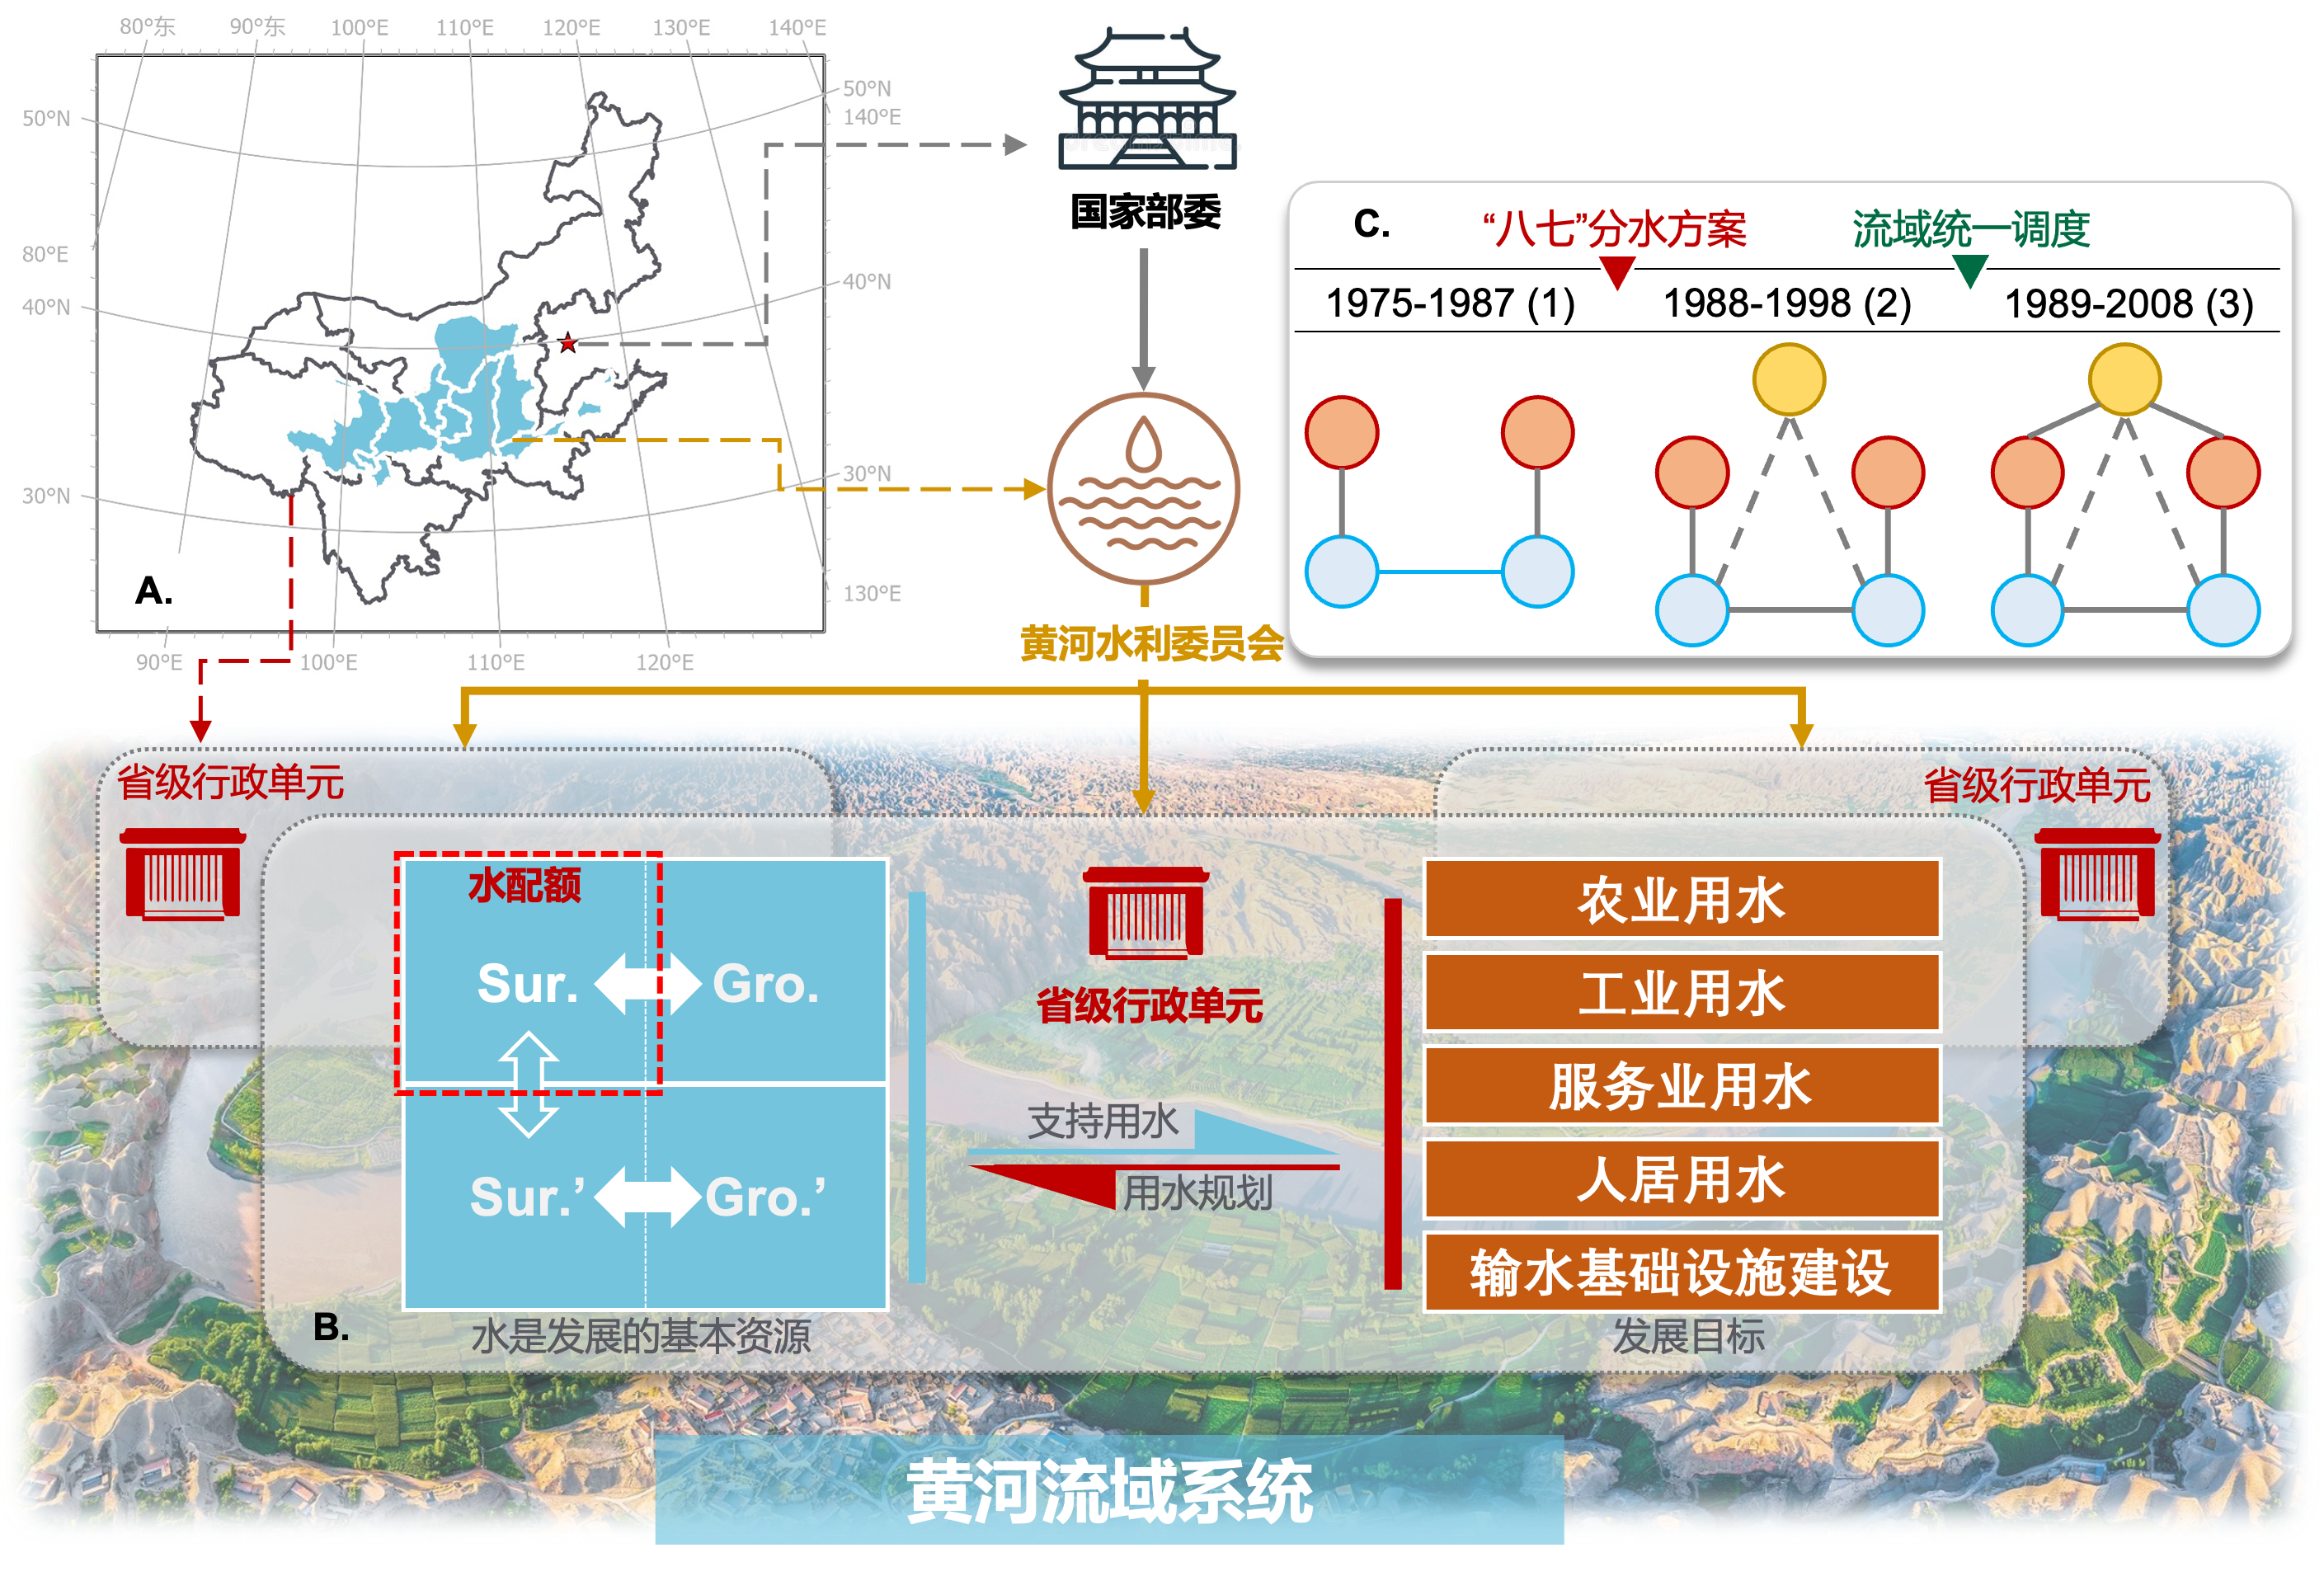
\includegraphics[width=\linewidth]{img/ch5/ch5_diagram.png}
	\caption[黄河流域社会-生态系统的分水制度结构及其变迁]{
		黄河流域社会-生态系统的分水制度结构及其变迁。
		\textbf{A.} 黄河流域跨越$10$个省(地区),其中$8$个对黄河流域水资源的依赖程度较高。国家部委(水利部)是发布水治理政策的最高权力机构,这些政策通常由流域级机构黄河水利委员会和各省级机构执行。
		\textbf{B.} 地方省政府(水利厅、局)是水分方案中的主要的利益相关者。自“八七”分水方案以来,由于黄河地表水的取用受到配额限制,利益相关者规划和利用水资源进行发展受到影响。自然水文过程是相互联系的,尽管配额制度主要限制地表水($Sur$),也可能通过社会水文过程影响流域内地下水($Gro$)或流域外地表水和地下水($Sur'$和$Gro'$)。
		\textbf{C.} 制度变迁和随之而来的社会-生态系统结构变化:
		(1) $1979 \sim 1987$年间,各利益相关方(红圈)从连接的生态单元(黄河河段,蓝圈)自由获取水资源。
		(2) 1987年施行“八七”分水方案后,黄河水利委员会(黄圈)负责监测各河段利益相关者用水情况。
		(3) 1998年施行“流域统一调度”之后,利益相关者必须向黄河水利委员会申请用水许可证(红黄圈之间的连接)。}\label{fig:structure}
\end{figure}

% 制度变动综述
1987年实施的“八七”分水方案和1998年实施的“流域统一调度”是黄河流域水治理中被广泛认可的里程碑事件。
在“八七”分水方案之前,参与分水方案的黄河流域各省份或地区可以根据其取水能力自由使用黄河的水资源进行开发,流域管理机构,即黄河水利委员会与这些地区在用水方面没有联系(图~\ref{fig:structure}~C)。
为缓解水资源压力,国家部委在“八七”分水方案中提出黄河流域$10$个省或地区之间应参照指定配额来取用水资源,且该配额与各省的预期取水量相去甚远(表~\ref{ch5:tab:quota})。
同时根据官方文件中的要求,黄河水利委员会需开始报告各省或地区和各个河段的用水情况。
这是黄河流域水利枢纽的责任首次涉及水资源利用,在社会与生态节点之间引入了新的联系(图~\ref{fig:structure}~C)。
由于备受争议的“八七”分水方案在此后十年内都没能解决黄河断流问题,1998年水利部签署同意了另一项制度变化——流域统一调度,强化了黄河水利委员会在综合管理用水方面的职责。
此次官方文件明确指出,各省须将其年度用水计划向黄河水利委员会报备并申请用水许可证,否则不再能使用黄河干流水资源,黄河水利委员会因此在社会-生态系统结构中同各省直接联系在一起(图~\ref{fig:structure}~C)。
综上所述,两次制度转换重塑了黄河流域水资源利用的结构,形成的三类具一般性的社会-生态系统结构块如图~\ref{fig:structure}~C所示。

% Table generated by Excel2LaTeX from sheet '八七分水方案配额'
\begin{table}[htbp]
    \caption{八七分水方案水资源配额}
      \begin{tabularx}{\textwidth}{LLLLLLLLLLL}
      \toprule
            & \multicolumn{1}{l}{青海} & \multicolumn{1}{l}{四川$^b$} & \multicolumn{1}{l}{甘肃} & \multicolumn{1}{l}{宁夏} & \multicolumn{1}{l}{内蒙古} & \multicolumn{1}{l}{山西} & \multicolumn{1}{l}{陕西} & \multicolumn{1}{l}{河南} & \multicolumn{1}{l}{山东} & \multicolumn{1}{l}{津冀$^b$} \\
      \midrule
      规划需求  & 35.7  & 0     & 73.5  & 60.5  & 148.9 & 115   & 60.8  & 111.8 & 84    & 6 \\
      1983年方案 & 14    & 0     & 30    & 40    & 62    & 43    & 52    & 58    & 75    & 0 \\
      1987年方案 & 14.1  & 0.4   & 30.4  & 40    & 58.6  & 38    & 43.1  & 55.4  & 70    & 20 \\
      多年平均耗水$^a$ & 12.03 & 0.25  & 25.8  & 36.58 & 61.97 & 21.16 & 11.97 & 34.3  & 77.87 & 5.85 \\
      黄河水在地区总用水的占比 & 48.12\% & 0.10\% & 30.79\% & 58.45\% & 47.82\% & 73.55\% & 44.39\% & 24.77\% & 34.41\% & 3.11\% \\
      \bottomrule
      \end{tabularx}\label{ch5:tab:quota}%
      \footnotesize
      $a$ 使用1987年到2008年数据计算,四川因数据不足,使用2004到2017年数据计算。
      $b$ 由于取自黄河流域的水资源占省(或地区)总用水量的比值太小($< 5\%$),不在本研究中进行考虑。
\end{table}%


\section{制度变化对用水的影响}

\subsection{主成分提取结果}

具有解释力的变量是构建稳健的合成控制方法的关键。
本章使用了与用水相关的$24$个变量(见表~\ref{ch5:tab:data_source}),这些数据集在先前的研究中已用于解释中国用水的变化\cite{zhou2020};由于这些变量之间存在相关性,使用主成分分析进行降维并增强合成控制方法的稳健性。
研究发现采用肘部法确定$5$个主成分时,能解释$89.63\%$的方差变异。
其中第一个主成分解释$51.6\%$的方差变化,第二个主成分解释$16.9\%$的方差变化。
这两个主成分是对区域用水量影响最大的两个轴,其余主成分对用水量的解释力均低于$10\%$。

% \begin{figure}[!h]
%     \centering
%     \includegraphics[width=0.6\textwidth]{img/ch5/ch5_elbow.png}
%     \caption{主成分分析的方差解释率肘部图}\label{ch5:fig:elbow}
% \end{figure}

使用双变量图同时展示数据集中样本点和变量特征,可以发现解释力最大的前$10$个特征大多和第一个主成分呈正相关(图\ref{ch5:fig:biplot})。
其中工业相关的自变量,如造纸、石化、纺织等高用水行业与第一个维度呈高度正相关;农业相关的自变量则仅呈现微弱正相关,但与第二个主成分呈高度相关(水稻正相关,小麦、玉米及其它农业负相关),可见主成分维度基本能够反映不同的区域的用水特征。
分析各特征在五个主成分上的负荷,可大致可将用水变量分为城市经济、农业灌溉、节水设施、气候适应、高耗水产业这五个类别(图~\ref{ch5:fig:variables})。


\begin{figure}[!h]
    \centering
    \includegraphics[width=0.6\textwidth]{img/ch5/ch5_biplot.png}
    \caption[主成分分析前两个主成分的双变量图]{主成分分析前两个主成分的双变量图(图中点为各省数据,x代表离群样本)}\label{ch5:fig:biplot}
\end{figure}


\begin{figure}[!h]
    \centering
    \includegraphics[width=\textwidth]{img/ch5/ch5_variables.png}
    \caption{区域用水量各主成分的特征显著性}\label{ch5:fig:variables}
\end{figure}

\subsection{合成控制结果}\label{result-2}
% 结果一:展示制度转变带来的用水量变化

黄河流域的总用水量在反事实推断模型和实际观测值在两次制度变化后呈现出差异显著,在之前此差异则较小且不显著(见图\ref{ch5:fig:main_results}A和B),这表明其用水变化的估计重建良好。
在1987年“八七”分水方案政策实施后,用水量变化速度的观测值为$1.82~km^3/yr$,比预测值$0.73~km^3/yr$高出$148.48\%$。
政策实施后$10$年间观测总用水量为$938.06~billion~m^3$,而预测值仅为$887.05~billion~m^3$,观测值比预测值高出$5.75\%$。
$T$检验结果显示在政策实施前,观测与预测之间用水量差异的$p$统计量为$0.93$,在政策实施后则下降至$0.003$,说明在政策实施前没有显著差异,但在政策实施后差异显著。
对用水量的理论估计表明,“八七”分水方案的制度转变促使各省取用了更多的水资源(图~\ref{ch5:fig:main_results}~A)

在$1998$年流域统一调度政策实施后,用水量的变化速度$-0.66~km^3/yr$,模型预测值则为$0.55~km^3/yr$,观测值比预测值低出两倍($-219.59\%$)。
在政策实施后的$9$年中($1998 \sim 2008$年),观测总用水量为$871.80~billion~m^3$,比预测值$931.08~billion~m^3$低$-6.37\%$。
$T$检验结果表明,政策实施前观测与预测间用水量差异的$p$统计量为$0.86$,在政策实施后为$0.002$。
同样说明在政策实施前没有显著差异,在政策政策实施后则差异显著。
可见在1998年流域统一调度制度出台后,用水量持续增加的趋势得到扭转(图~\ref{ch5:fig:main_results}~B)。

\begin{figure}[!h]
	\centering
	\includegraphics[width=\linewidth]{img/ch5/ch5_results.png}
	\caption[黄河流域两次水资源分配制度变化的影响]{
        黄河流域两次水资源分配制度变化的影响。
        \textbf{A.} “八七”分水方案前后黄河流域用水量($1 \times 10^9~m^3$);
        \textbf{B.} 流域统一调度前后黄河流域的用水情况。蓝线是来自统计资料的用水量,灰色线为经济和环境背景控制下差分合成控制法的估计值;
        \textbf{C.} 黄河流域干旱强度与断流事件,灰色气泡的大小表示断流河段的长度。
	}\label{ch5:fig:main_results}
\end{figure}

“八七”分水方案后用水量的增加与$1987 \sim 1998$年日益严重的黄河断流相一致,无论是断流时长还是断流河段长度都在此时期持续增加,导致流域生态退化危机(图~\ref{ch5:fig:main_results}~C)。
但在$1998$年流域统一调度之后,立竿见影地结束了长达二十余年的河流断流。
尽管$1998 \sim 2008$年黄河流域的平均干旱强度高于$1987 \sim 1998$年(平均干旱指数从$0.47$提升至$0.62$,图~\ref{ch5:fig:main_results}~C)。
这再一次证明了1987年提出“八七”分水方案最初没有有效限制用水,直到1998年的流域统一调度制度才成功限制了用水。

\subsection{鲁棒性检验}

对上述合成控制法拟合的结果进行鲁棒性检验,结果如图\ref{fig:87placebo}和图\ref{fig:98placebo}所示,柱状图长度代表政策实施后与政策实施前的均方根误差之比,该比值越高则说明合成控制法的效果越好。
黑色为该区域的合成控制结果,灰色为所有安慰剂对照组,红色区间则是所有安慰剂对照均值的$95\%$置信度区间,黑色柱状图高于该红色区间则说明该区域效果显著好于安慰剂对照,即有超$95\%$的把握说明政策干预对该区域的影响是明显的、且合成控制法有效模拟了此影响。
在$1987$年“八七”分水方案政策实施后,河南、甘肃、内蒙古自治区的合成控制效果显著高于其它安慰剂实验组($p < 0.05$),这说明分水方案对这三个省份的用水有着显著作用;山西、陕西显著低于其它控制对照组,其余省份均无显著差异,说明政策干预对这些地区没有明显效果。
在$1998$年流域统一调度政策实施后,除了河南和内蒙古自治区的合成控制效果显著低于安慰剂实验组外($p > 0.05$),其余省份都显著高于安慰剂实验组,这说明$1998$年的政策干预对河南与内蒙古的用水没有显著影响;其余省份均受到该制度的强烈干预,促使用水量减少。

\begin{figure}
    \includegraphics[width=0.9\linewidth]{img/ch5/ch5_rmse_87.png}
    \centering
    \caption[“八七”分水方案政策干预的安慰剂检验]{“八七”分水方案政策干预的安慰剂检验。深色柱子是当前省份的实验后/前均方根误差之比,灰色柱子是对所有非黄河流域其他省份构建合成控制模型得到的均方根误差之比,红色是$95\%$置信区间。深色柱子若落在该区间内,则说明该省份的合成控制模型与流域外省份相比不具有显著差异。}\label{fig:87placebo}
\end{figure}

\begin{figure}
    \includegraphics[width=0.9\linewidth]{img/ch5/ch5_rmse_98.png}
    \centering
    \caption[流域统一调度政策干预的安慰剂检验]{流域统一调度政策干预的安慰剂检验。深色柱子是当前省份的实验后/前均方根误差之比,灰色柱子是对所有非黄河流域其他省份构建合成控制模型得到的均方根误差之比,红色是$95\%$置信区间。深色柱子若落在该区间内,则说明该省份的合成控制模型与流域外省份相比不具有显著差异。}\label{fig:98placebo}
\end{figure}


\subsection{各省的净效应差异}\label{result-3}

% 结果2部分:展示区域相应差异
研究结果表明各省(地区对这两次水资源分配制度变化的响应模式存在差异。
图\ref{fig:regulating}中,红色柱状图(“八七”分水方案)和绿色柱状图(流域统一调度)分别表示在该制度转变后的十年内,实际用水量相对于反事实推断模型估计值的增减比例;灰色柱状图显示了在两次制度转变后的十年内,各省实际用水量相对于其总用水量的比例;三角形标记指示“八七”分水方案为该省制定的理论水资源配额所占黄河流域总可用水量的比值。
在“八七”分水方案后的十年间,各省用水量相对反事实推断模型所估计用水量增加(或减少)的比例与其当前从黄河流域的取用水占比呈正相关(偏相关系数为$0.64$,图~\ref{fig:regulating})。
从1987年到1998年,一些用水大省(如内蒙古、河南、山东)也出现了显著的用水量增加(图~\ref{fig:regulating}),山东、内蒙古、河南和宁夏四省的用水量平均比预测值高出$32.14\%$。
而在施行流域统一调度后的1998年至2008年,几乎所有省份的用水量都出现了下降(平均下降$16.54\%$),
且各省用水量与从黄河流域的取用水占比变成了负相关(偏相关系数为$-0.51$)。

\begin{figure}[!h]
	\includegraphics[width=\textwidth]{img/ch5/fig3.png}
	\caption[分水制度变化对黄河流域各省影响的差异]{分水制度变化对黄河流域各省影响的差异}\label{fig:regulating}
\end{figure}


% \section{讨论}\label{ch5:discussion}
% discussion-1:
% 用水量的上升、下降-结果解读
% 制度对社会生态系统的结果产生影响在世界范围内都很普遍,
\subsection{制度变迁:深远影响流域的演变}

制度对社会-生态系统结果的影响在世界范围内被广泛报道,但很少有人试图量化其净效应\cite{cumming2020a}。
结果表明,流域统一调度降低了黄河流域的用水量,而“八七”分水方案增加了$8.57\%$。这一结果对之前的分析提出了挑战,即表明“八七”分水方案“几乎没有实际影响”,因为从理论上讲,如果没有影响,那么黄河流域的实际用水和合成用水之间应该没有什么差距\cite{abadie2015,hill2021}。
然而,我们的分析表明,“八七”分水方案的显著净效应表明,即使在控制了环境和经济变量之后,也会有更多的用水量。
相反,流域统一调度减少了地表水竞争,因此许多研究将河流流量的恢复主要归因于该制度的成功引入\cite{chen2021,huangang2002,an2007}。

% 实证研究表明,在社会经济系统中,这种广泛存在的构建模块是结构功能的关键。基于网络的方法是将实体之间的连接抽象为链接和节点\cite{bodin2017a,kluger2020,guerrero2015}。
%
% discussion-2: 87的增加
% 结果与制度的目的完全相反的“八七”分水方案与许多其它的SES失败治理案例类似,表明不匹配的社会生态结构可能促进了对公共资源的掠夺式开采。
“八七”分水方案的结果与该制度的目标相悖,与许多其他社会生态系统治理失败的情况相似,证明不匹配的社会生态结构会加剧共同资源的恶化\cite{kellenberg2009,cai2016,barnes2019}。
在“八七”分水方案实施后,用水量的增加与一些省份频繁争夺水资源的担忧是一致的。
尽管“八七”分水方案效果不理想的原因已经得到广泛的讨论(如执行、可行性和公平性),但是结构变化的关注却有限。
我们的结果表明,在“八七”分水方案实施后,目前的用水量与变化用水量(增加或减少)之间存在显著的相关性(图\ref{fig:regulating})。
这种“主要用户使用更多”的模式支持这样的假设:独立的利益相关者(如个别省份)将通过最大化效用来适应结构变化。

我们的理论分析得到了两个事实的支持:
(1) 在“八七”分水方案的配额讨论中,各个利益相关者(如各个省份)试图展示他们与水资源利用相关的发展潜力,因此在1982年到1987年间进行了“讨价还价”的过程\cite{wang2019a, wang2019d}。
这个“讨价还价”的过程也是一个将水资源配额与经济总量相匹配的过程,因为如果只考虑经济潜力的话,主要用水户(如山东和河南)需要的水资源超过了他们原先的配额\cite{zuo2020}。
(2)由于决策者与利益相关者之间的信息不对称,目前用水量较高的省份在水资源分配中具有更强的讨价能力。因此,利益相关者有相当大的动机来防止水配额阻碍他们的经济潜力,这与他们向中央政府要求更多水资源的呼吁是一致的\cite{wang2019a, wang2019d}。

\subsection{结构匹配:制度影响的内在机制}

本研究的结果对于改善流域社会-生态系统的治理具有重要启示。
通过流域统一调度,黄河流域水利枢纽可根据水文情况调整整个流域地表水利用指标。
当黄河水利委员会开始协调利益相关者时,各省外部对提高配额的请求变为内部创新,以提高用水效率(例如,大量增加节水设施)\cite{krieger1955, ostrom1990},研究结果表明这种流域尺度的制度匹配对于减少用水是必要的。
然而,由于流域统一调度仅规范地表水的使用,有许多证据表明,由于水需求得不到满足,制度转变可能导致更广泛的级联效应。
例如,文献估计,在许多灌区,流域统一调度后地下水取水量增加,可惜少有关于地下水使用的合格数据,难以用数据分析的方法开展进一步研究\cite{sun2022b}。
近年来,全国范围内开始实施类似的水配额政策,这改变了社会行动者与资源单位之间的关系。由于本研究中的两种制度变革都在社会-生态系统内部引发了意料之外的变化或级联效应,所以更好的管理需要对耦合的人类和自然系统进行更多的制度分析。

我们这里描述的结构构建单元(或图模型)(参见图~\ref{fig:structure})在全球范围内的其他社会-生态系统中也有报道。
在流域统一调度之前,SES结构(即独立的社会行为主体与生态系统片段相关联的单元)更有可能不协调,因为孤立的行为主体通常难以保持生态系统整体的相互关联\cite{sayles2017,sayles2019,cai2016,bergsten2019}。
流域统一调度后,制度调整增强了黄河水利委员会的权威,帮助其与黄河流域的资源供应规模相匹配,从而提高了社会-生态的适应性,并在改善径流方面取得了更好的效果\cite{cumming2020a,wang2019d}。
这再次证明了在耦合的人类-自然系统中寻求双赢局面的困难\cite{hegwood2022},以及更深入了解社会-生态结构的必要性\cite{bergsten2019, sayles2019}。
因此,黄河流域的案例可以更深入地解释先前的SES结构构建单元的协调和不协调,通过合理的因果关系和潜在过程将SES结构和结果联系起来。

% \subsection{Limitation, insights and implications}
\subsection{研究不足与未来展望}
% % 江恩慧 2022本子
% 随着黄河流域生态保护和高质量发展重大国家战略的深入实施,黄河流域社会经济从“高速发展”进入了“高质量发展”阶段,需从过去对水资源的过度开发和粗放式利用转向产业结构优化调整下的节约集约利用,对流域水资源配置提出了更高要求。然而,黄河水资源开发利用程度高达80\%,甚至在西北部分地区达到了100\%,已触及水资源供给的“天花板”(王建华等,2020);沿黄城市发展高度依赖黄河水资源配置,且已有90\%以上城市处于水资源超载状态(李原园等,2021);未来水资源供需矛盾有可能进一步加剧。

我们的方法存在一些必然的局限性。
首先,由于因果关系的相互交织,很难分辨经济增长和制度变革的贡献。其次,在使用DSC方法时,很难排除其他政策在同一时间断点(1987年和1998年)上的影响。
尽管如此,我们的实验方法提供了证据,证明在黄河流域的独特制度变革后,水的使用模式发生了变化,并对水管理提供了深刻的见解(特别是关于拥有一个与流域规模匹配的、全流域的水分配解决方案的权威重要性)\cite{bodin2017b, ostrom2009, reyers2018}。
此外,流域统一调度制度变革的最终成功从理论和实践上证明了社会-生态匹配的重要性。
因此,为了未来的可持续性,有必要强调与生态系统规模相一致的主体加强利益相关者之间的联系的必要性。
% 如果用边际效应分析的话,加入以下内容
% 从这些角度来看,基于边际效益分析(见\textit{\nameref{secS5}})的两种情况可以启发如何减少不匹配的制度设计。
% 例如,水权转让可能是在利益相关者之间建立横向联系的另一种方式,这也有可能导致更好的水治理。
% 此外,政策制定者可以提出更有活力和更灵活的制度,以增加利益相关者对不断变化的社会经济环境的适应\cite{reyers2018}。

全球生态-社会系统的结构模式是影响结果的关键因素,因此我们提出的机制对于治理这种耦合系统至关重要。
最近,黄河流域重新设计水分配制度的呼声也说明了制度解决方案对可持续性的关键性。
随着不断变化的环境背景,旧有的水资源分配制度已经不能满足可持续发展的要求,因此中国政府已经开始规划重新设计其历史悠久的水资源分配制度\cite{wang2019a}。
我们的分析表明,如果模式不匹配,新制度的建立可能会导致系统扭曲。
因此,我们的研究为如何解决不正当激励问题提供了一个重要的教训,而黄河流域的经验可以为全球生态-社会系统的管理提供指导\cite{hegwood2022, muneepeerakul2017, leslie2015}。


\section{小结}\label{ch5:summary}
通过制度(如政策、法律、和社会规范)来重塑社会-生态结构,是流域系统人水关系变化的重要驱动力,时空匹配的制度能够达到预期的水治理目标,支持流域高质量、可持续发展。
本章重点关注$1987$年的“八七”分水方案和$1998$年的“流域统一调度”两次自上而下的水资源分配制度变化,分析它们重塑流域系统社会-生态结构的过程,定量识别其对流域用水的影响。

本章厘清了两次水资源分配制度变化前后黄河流域的社会-生态结构,发现流域尺度的黄河水利委员会在制度变化后,引入了与生态节点和其它社会节点之间的新联系,形成了不同的结构模式。
使用“差分合成控制法”的因果推断模型进行反事实推断,考虑经济增长和气候条件,估算“假设没有制度干预”情景下的理论用水量,表明“八七”分水方案的制度变化显著($p<0.05$)促使黄河流域在接下来十年内多用了约$5.75\%$的水资源;而流域统一调度制度后,流域总用水量以每年$6.6$亿立方米的速度下降,远小于模型预测的每年$5.5$亿立方米的增速,展现出良好的治理效果。

本章研究表明社会-生态系统结构失配可能使会制度产生背离预期的结果,强调了保持治理系统尺度匹配的重要性,本章黄河流域分水制度的治理案例可为全球大河流域提供借鉴和指导。

\label{chapter5}

	\chapter{流域人水关系演变的响应机制建模}
% 第五章研究表明,黄河流域的分水制度变化会深远影响流域不同地区的用水量。
% 但$1987$年提出的“八七”分水方案与限制用水的预期相悖,直至$1998$年“流域统一调度”的制度变化才成功限制用水,解决了黄河的断流问题,且尚不清楚这是否会带来新的生态问题,如替代性地增加地下水开采。
% 此外,上层决策通常反映着下辖区域不计其数利益相关者的诉求,仍需要从具体用水者的角度出发,自下而上深入分析和模拟其中机制。
% 本章进一步聚焦黄河流域地表用水量最多的农业部门,通过模拟各地区不同来源的灌溉用水如何响应制度变化,回答上述具体问题。

本章建立了自下而上的多主体模型,从不同尺度(灌溉单元、用水集体、行政单元)建立反馈过程,模拟黄河流域农业灌溉用水者对$1987$年和$1998$年两次分水制度变化的响应差异。
模型包含了基于公共池塘资源演化博弈的人类模块、模拟作物需水的自然模块,并使用“基于主体的社会-生态系统框架”(ABSESpy)建立人类-自然模块的耦合关系。
通过该耦合模型,本章可以模拟小麦、玉米、水稻三种主要粮食作物种植用水来源,在月尺度区分为自然降水、地表水、地下水,从而分析分水制度变化对各类水资源开采量的影响。


\section{研究方法与数据来源}
% 本章研究聚焦于用水者决策过程与环境之间的反馈过程进行建模。
% 使用多主体模型黄河农业灌溉主体对流域水资源分配制度的决策过程,并从“主体规则的设计”、“模块构建与耦合”、“数据输入与分析”三个方面介绍本章的研究方法。

\subsection{主体规则的设计}

本小节将分别从个体尺度、地区尺度、流域尺度介绍多主体模型的规则设计,三者的关系如图\ref{ch6:fig:framework}所示:
(1)个体尺度的灌溉主体是进行农业生产的基本单位,基于环境信息和制度条件做出具体、实际的用水决策;
(2)地区是灌溉主体接受制度规制的主要尺度,流域系统的制度变化通过此级规则落实到主体间交互之中;
(3)流域尺度则约束了模型允许的环境背景,例如主体分布、水文气候条件、主体交互网络。
% 模型的主要目的是分析流域水资源分配制度如何影响农业灌溉主体的用水来源:用多少地下水?
% 将小麦、玉米、水稻三种主要粮食作物种植用水来源在月尺度区分为自然降水、地表水、地下水,并分析了地表分水制度变化对地下水开采量的影响。

\begin{figure}[htb]
    \centering
    \includegraphics[width=0.8\textwidth]{img/ch6/ch6_framework.png}
    \caption[多主体模型的设计框架]{多主体模型的设计框架。
        \textbf{A.} 自然模块:水文气候条件、流域主体的作物选择和灌溉策略如何影响作物蒸散发。
        \textbf{B.} 人类模块(个体尺度):流域内的灌溉主体在给定水文气候条件、给定配额上限/下限的情况下如何决定其用水来源及用水量;
        \textbf{C.} 地区尺度:体现制度变化对区域总可用水配额的影响。
        \textbf{D.} 流域尺度:体现流域系统的主体分布、主体网络结构特征对主体博弈决策的影响。
    }\label{ch6:fig:framework}
\end{figure}

\subsubsection{个体尺度}

对单个灌溉主体而言,灌溉引水决策的核心是对作物在天然降水之外的水亏缺进行人为补给。
水亏缺是考虑灌溉损失后的作物蒸散发与实际降水量之间的差,作物蒸散发则采用国际粮农组织(FAO)推荐的单作物系数法进行计算,由潜在蒸散发和作物蒸散发系数计算得到。

\begin{equation}
    \label{ch6:eq:deficits}
    W_{deficits} = \frac{ET_c - P}{k_{loss}}
\end{equation}

\begin{equation}
    \label{ch6:eq:etc}
    ET_c = ET_{0} * Kc
\end{equation}

其中潜在蒸散发和降水根据主体所处的位置直接从自然模块调用相应属性,作物蒸散发系数$Kc$的同样通过查阅采用国际粮农组织($FAO56$)推荐的作物表得到(表\ref{ch6:tab:crops})。


% Table generated by Excel2LaTeX from sheet '作物物候表'
\begin{table}[htbp]
    \centering
    \caption{模拟黄河流域主要粮食作物物候表}
      \begin{tabularx}{\textwidth}{p{1.5cm} LLLLL p{1cm} p{1cm} p{1cm}}
      \toprule
      作物名称  & \multicolumn{1}{l}{播种期} & \multicolumn{1}{l}{萌发期} & \multicolumn{1}{l}{生长期} & \multicolumn{1}{l}{中期} & \multicolumn{1}{l}{后期} & \multicolumn{1}{l}{$Kc_{ini}$} & \multicolumn{1}{l}{$Kc_{mid}$} & \multicolumn{1}{l}{$Kc_{end}$} \\
      \midrule
      小麦    & 4月5日  & 4月25日 & 5月20日 & 7月19日 & 8月18日 & 0.15  & 1.15  & 0.30  \\
      水稻    & 4月15日 & 5月15日 & 6月14日 & 7月14日 & 8月13日 & 1.00  & 1.20  & 0.70  \\
      玉米    & 4月19日 & 5月9日  & 6月13日 & 7月23日 & 8月22日 & 0.15  & 1.20  & 0.50  \\
      \bottomrule
      \end{tabularx}\label{ch6:tab:crops}%
\end{table}%


但在农民生产实际中,基本不可能做到完全按照作物的水亏缺决定灌溉量,而是根据经验,既往文献中通常在水亏缺基础上额外使用一个系数$\alpha$表示实际决策中的灌溉量,该系数估计了农民对作物水亏缺的经验认知与节水灌溉的影响,即实际灌溉用水量$WU$可表示为:

\begin{equation}
    \label{ch6:eq:WU}
    WU = W_{deficits} * \alpha
\end{equation}

但在本章研究中,由于时间跨度较长($1980 \sim 2010$),区域灌溉的节水升级改造是响应制度变化的重要措施,系数$\alpha$一定是剧烈变化的。
因此,本章研究根据用水量$WU$的年际统计数据将尺度下降到月尺度,$WU_i$代表农民在作物生长季在第$i$个月的实际的用水需求,而经验系数$\alpha$的值则可以作为反映灌溉节水的指标,则有:

\begin{equation}
    \label{ch6:eq:WUi}
    WU_i = WU * \frac{W_{deficits, i}}{\sum_{i} W_{deficits, i}}
\end{equation}

其中$i$为模型的每个时间步长单位(月),因此在每步模拟中,可将每个灌溉主体的作物生长用水来源$W$分为降水来源$W_p$、地表水来源$W_s$、地下水来源$W_g$三部分,具体用水决策及模型计算顺序如下:
(1)根据降水和作物蒸散感知水亏缺$W_{deficits}$,如果$W_{deficits}=0$,说明降水已经满足了需求,则作物生长水源$W$就完全由降水提供,$W=W_{p}$;
(2)如果降水无法满足作物生长需求,就根据公式\ref{ch6:eq:WUi}评估当月的水需求$WU$,并设定降水来源$W_{p} = P$;
(3)对于需求$WU > 0$,假定农民首先考虑从地表水获得,根据自己的官方配额$Q_{0}$和超采的配额$Q_{1}$决定多取用多少配额$Q = Q_{0} + Q_{1}$,若$Q > WU$,则地表水使用$W_s = WU$,否则$W_s = Q$;
(4)最后估计地表水开采量$W_g$,所有降水和地表水仍不被满足的用水需求都被认为从地下水获取,即$W_g = WU - W_s - W_p$。

\subsubsection{地区尺度}

黄河流域的配额制度通常仅细致到地级市范围,如何在地区尺度分配该地区的可供分配的水资源配额取决于主体之间的自组织。
本章研究中假设地区尺度完全根据作物的水亏缺$WU_{deficits}$分配灌溉水量,作为完全的“按需分配”,这是节约配额的理论最优(也是理论最公平的)情景,这也意味着现实中的资源供需匹配不会比本章研究的模拟结果更好。
在数学上,假设总地表水配额为$Q_{C}$的地区$C$中包含$n$个主体,则主体$j$的配额$Q_j$为:

\begin{equation}
    \label{ch6:eq:quota}
    Q_j = Q_{C} * \frac{W_{deficits, j}}{\sum_{j \in C} W_{deficits, j}}
\end{equation}

由于第五章中介绍的分水制度差异及其变化,地区$C$的配额并非固定不变的,在$1987 \sim 1998$年间水资源配额存在可浮动的特性,使用$Q_{\min}$和$Q_{\max}$两个属性进行表达,允许用水个体的实际地表取用水在其间浮动。
$Q_{\max}$由黄河流域各省在$1983$年自主上报的水资源配额需求基础上降尺度到地区和月份来估算(详见表\ref{ch5:tab:quota}),代表自主取水时期满足该地区主体用水需求的能力上限,通常这是官方建议配额$Q_{\min}$的近两倍。
因此,关于$Q_j$的判定规则如公式\ref{ch6:eq:which_quota}所示,与模型当前模拟的年份$yr$有关:

\begin{equation}
    \label{ch6:eq:which_quota}
    Q_j =
    \begin{cases}
        Q_{\max} & \text{when } yr < 1987 \\
        Q_{\in} \leq Q_j \leq Q_{\max} & \text{when } 1987 \leq yr \leq 1998 \\
        Q_{\min} & \text{when } yr > 1998
    \end{cases}
\end{equation}

在$1987 \leq yr \leq 1998$时期,每个主体在计算配额$Q$时如果有较大的用水需求,其$Q_{0} = Q_{\min}$会保证被优先满足,因为这是分水方案中明确保证的合法配额。
由于这个配额没有被强制执行,该主体拥有一定的灵活性索取获得超越官方建议配额$Q_{\min}$的额外配额$Q_{1}$,即超出制度规定但不违背需求上限的“违背制度”部分,该部分配额的值与主体的社会属性有关,详见\ref{ch6:sec:society}部分的模块介绍。
但$Q = Q_{0} + Q_{1}$不会超过该主体能被分配到的最大合理配额$Q_{\max}$。

\subsubsection{流域尺度}

在流域尺度,需要决定主体生成的数量、位置、以及相互作用网络。
气候、水文、人口的空间数据精度同化至$0.1$度,即每个空间栅格的范围大约为$A_{cell} = 121{km}^2$,这也是主体进行灌溉活动的基本单元。
本章研究的时间精度是月,考虑作物的生长季主要在$4$月到$8$月之间(见表\ref{ch6:tab:crops}),因此根据统计数据中三类主要作物的灌溉面积和模拟的空间精度来估计每个地级市的主体数量。

\begin{equation}
    n_{C} = \sum_{k=R, M, W}\frac{A_{C, k}}{A_{cell}}
\end{equation}

其中$k = R, M, W$分别代表本研究考虑的三种作物:水稻、玉米和小麦,$A_{C, k}$为该种作物在$C$市的灌溉面积,$A_{cell}$则为每个斑块(栅格)代表的面积。
由于各地级市的面积每年都会变化,主体数量也会每年使用新的统计数据来进行更新。
每个栅格只能同时存在一个主体,在保证主体数量与灌溉面积一致的基础上,主体生成的位置是随机的,概率遵循以人口空间分布的加权平均。

主体决策之间会互相影响,每年的主体数量和位置更新后,还需要预设主体之间的交互关系。
以每个主体为一个节点,存在相互影响的主体间存在连边,那么整个流域可形成一个复杂网络,该网络可包括三种潜在连边:
(1)同一地级市的灌溉主体之间
(2)不同地级市的灌溉主体之间
(3)不同省区的灌溉主体间
由于中国农业基本单元的封闭性,本研究假设不同省之间的主体之间不会互相影响(即不会出现跨省互相影响决策的情况),在同一地级市之内和地级市之间的连边遵循具有固定连边概率的ER随机图(Erdős–Rényi random graphs)构建算法(Erdos and Renyi, 1959),即随机图是一个由$C * n$个节点组成的图,其中同一地级市每对节点连接的概率为$p_n$,不同地级市之间则每对节点的连接概率为$p_C$。
因此一旦概率对$p_n$,$p_C$给定,全流域范围内所有灌溉主体之间可能互相影响的网络拓扑关系就被确定了。

\subsection{模块构建与耦合}

在上述规则构架下,本研究包括两个关键模块:
(1)人类模块:流域内的灌溉主体在给定水文气候条件、给定配额上限/下限的情况下如何决定其用水来源及用水量;
(2)自然模块:水文气候条件、流域主体的作物选择和灌溉策略如何影响作物蒸散发。
本节先分别介绍两个模块的运行过程,最后介绍二者间的耦合反馈关系。

\subsubsection{人类模块}\label{ch6:sec:society}

在人类模块中,本研究使用演化公共池塘博弈的分析框架对主体面对配额限制的决策响应进行分析,使用遵循配额($C$)与违背配额($D$)来概括主体在面对灵活水配额制度($1987$年至$1998$年间)的基本决策。
博弈论(Game Theory)是研究决策者之间战略互动的数学模型,是研究具有竞争性质现象的理论和方法,对于公共水配额这种竞争性、排他性都很强的的“公共池塘资源”,符合演化公共物品博弈的模型框架\cite{ostrom2009, traulsen2010}。
演化公共池塘博弈框架又称多代理人囚徒困境博弈,本研究中主体$i$选择是否遵循限制地表用水的配额制度($S_i = 1$表示合作$C$,$S_i=0$代表决策$D$)。
如果某个主体同意严格遵循配额制度$Q = Q_{\min}$,那么他将损失潜在收益$c$中的一部分。
如果每个人都遵循配额(选择合作$C$),那么共同投资的总额可能会变成原来的$r$倍,并在所有参与的投资者中平分。
如果有$N$个代理人参与,那么每个人的博弈收入$E$如由两部分组成(见公式\ref{ch6:eq:game}):$-c*S_i$ 代表单个主体对集体贡献的成本,而 $\sum_{j=1}^N S_j$则代表共同利益池给每个贡献的主体分到的利益。

\begin{equation}
    \label{ch6:eq:game}
    E=-c * S_i+\frac{r c}{N} \sum_{j=1}^N S_j=-\left(c-\frac{r}{N}\right) S_i+\frac{r c}{N} \sum_{j \neq 1}^N S_j
\end{equation}

在本研究中,黄河分水制度对于遵循配额的主体没有任何额外的经济补贴(这被视为一种行政上的义务行为),也没有正式的经济上的行政处罚,因此公共池塘的收益系数$r = 1$。
此外,因为黄河流域灌区的地下水取水的成本普遍高于地表取水,潜在成本$c$与地下水开采量$W_g$有关,使用$c \propto W_g = k_e * W_g$表示,本研究中为直观考虑采取经济系数$k_e = 0.3$,即意味着地下水水费每单位比贵$0.3$单位。
这个系数的取值实际上不会影响模型表现,因为本研究后续影响主体决策的是主体间的收入差距,而所有主体的潜在收益$E$与地下水取水量都是同样的线性关系,决定主体收益差距仅由地下水开采量$W_g$的差距决定。
因此理论上可预期的是,在响应制度的经济驱动因素上,遵循配额会产生大量地下水开采成本的地区将拥有更大的动机违背配额。

作为没有任何补贴的制度,影响主体是否遵循配额的另一个主要驱动因素是社会规范,因为即便没有经济惩罚,违背制度也是不被提倡的。
多元理性理论是一个理解个人决策与社会规范影响之间关系的经典框架,指出由“个体/集体主义”与“注重/轻视规范”两个维度,就可以预测不同文化背景下遵循社会规范的倾向\cite{verweij2015},因此可以对复杂的政策问题进行结构化的诊断,因此该方法框架已被应用于解释水治理的成功与失败。
参考 Castilla-Rho 等人基于多元理性(Plural rationality theory PRA)的社会理论的一系列研究,可以使用两个简单的参数$b$和$v$来测量主体遵循制度规范的动因。
其中$b\in[0, 1]$表征某主体“注重/轻视规范”的程度,在模型中也是该主体突破规定配额,做出决策$D$的概率。
$v \in [0, 1]$则表征主体“个体/集体主义”的程度,该参数越大代表主体越重视与他人保持一致,在模型中是对该主体社交网络中违规行为进行负面评判的概率。
考虑到人们不愿意主动得罪别人,也不愿意丧失名誉,这种评价将成为计算社会得分的基础,采用在福利经济学中常用的Cobb-Douglas函数的形式进行表达:
% Cobb-Douglas函数(https://inomics.com/terms/cobb-douglas-production-function-1456726)
% [Happy Planet Index](https://happyplanetindex.org/) 
% 人类发展指数(http://hdr.undp.org/en)
\begin{equation}
    S = {(grid)}^m * {(1 - group)}^n
    \label{ch6:eq:society}
\end{equation}

其中 $m$ 是一个主体发现其它人违规超配额用水的次数,$n$ 则是他被他人发现超配额用水的次数。
即$grid^m$ 这部分表达的是主体因周围人违背制度规范而感到不舒服;$group^n$ 这部分表达的是一个主体违背制度规范而被周围人指指点点而感到不舒服。
$grid$与$group$是反映社会整体平均$b$与$v$水平的参数。

在演化博弈中,决策还是可演化的(Evolutionary),因为一些反应因为符合社会规范而受到奖励,而另一些反应则因为背离社会规范而受到惩罚。
人类模块在每一个时间步的最后将计算所有主体的博弈结果——$0 \sim 1$标准化后的经济得分($E$)与社会得分($S$),并将两者平均$Score = E * S$作为主体的最终得分。
在社会网络中,表现最成功的主体决策以一定概率$p_{l}$被他的朋友们学习,学习后的主体使用被学习对象的$b$和$v$参数代替学习者原本的参数。

综上所述,在人类模块的每次模拟中,每个主体都将遵循图\ref{ch6:fig:society}所示的流程图:

\begin{figure}[htb]
    \centering
    \includegraphics[width=0.8\textwidth]{img/ch6/ch6_updates_diagram.png}
    \caption[多主体模型的更新规则与模拟流程]{多主体模型的更新规则与模拟流程。
    左侧表示多主体模型整体运行的大致流程,“更新社会”步骤是人类模块进行决策的部分,包括五个主要步骤:
        (1)主体根据自己当前的$b$属性(“注重/轻视规范”)作为选择合作的概率,决定本轮中使用的决策“C/D”。
        (2)若当前主体选择不合作(D),其余选择合作(C)的主体根据其$v$属性(“个体/集体主义”)决定是否对其进行社会规范上的谴责。
        (3)对每个主体按照谴责他人/被他人谴责的次数估计自己的社会收益$S$。
        (4)综合社会收益$S$和经济收益$E$,每个主体都将学习自己朋友中综合表现最好的个体,模仿他的$v$和$b$属性,若自己的表现就是朋友中最好的,则跳过此步骤。
        (5)为避免模型陷入局部最优,以极小概率($\alpha = 5\%$)对主体的策略进行变异,设置$v, b \in [0, 1]$成新的随机数。
    }\label{ch6:fig:society}
\end{figure}

\subsubsection{自然模块}

在自然模块中,本研究使用 FAO56 推荐的算法计算潜在蒸散发$ET_0$、作物蒸散系数$Kc$、以及作物蒸散发$ET_c$:

\begin{equation}
    ET_c = ET_0 * Kc * Ks
\end{equation}

其中$Ks$是水应力系数,主要与土壤质地有关。由于在本研究中仅考虑三种主要粮食作物,且主要分布在灌溉条件良好的土壤上,对此系数的空间分异不再作进一步考虑,使用系数$Ks = 0.3$进行估计。  % TODO chen 2023

潜在蒸散发$ET_0$的计算方法使用Penman-Monteith方法,式\ref{ch6:eq:pm}:

\begin{equation}
    \label{ch6:eq:pm}
    PET = \frac{0.408 \Delta (R_{n}-G)+\gamma \frac{900}{T+273}
    (e_s-e_a) u_2}{\Delta+\gamma(1+0.34 u_2)}
\end{equation}

其中$Rn$为作物表面上的净辐射,$MJ/(m^2 day)$;$G$为土壤热通量,$MJ/(m^2 day)$;$T$为$2$米高处日平均气温$^\circ C$;$u2$为$2$米高处的风速,$m/s$;$es$为饱合水汽压,$kPa$;$ea$为实际水汽压$kPa$;$es - ea$为饱和水汽压差,$kPa$;为饱和水汽压曲线的斜率;$r$为湿度计常数,$kPa/^\circ C$。
由于计算的时间尺度(月),土壤热通量可以忽略。根据其它数据可得性,对经验公式\ref{ch6:eq:pm}中的饱和水汽压$es$使用气温数据进行估算:

\begin{equation}
    e^0(T) = 0.6108 * \exp \frac{17.27 T}{T + 237.3}
\end{equation}

\begin{equation}
    es = \frac{e^0(T_{\max}) + e^0(T_{\min})}{2}
\end{equation}

作物生长期间的作物系数$Kc$的曲线是用三个阶段的作物系数来估计的:初期($Kc_{ini}$)、中期($Kc_{mid}$)和后期($Kc_{end}$)。
作物系数的各转折点以表\ref{ch6:tab:crops}中的数据为依据进行定位。
$Kc_{ini}$的计算方法如下\cite{allen1998}。

\begin{equation}
    \label{ch6:eq:kcini}
    K_{\text {c, ini}}=\frac{\mathrm{TEW}-(\mathrm{TEW}-\mathrm{REW}) \exp \left[-\left(\mathrm{t}_w-\mathrm{t}_1\right) E_{so}\left(1+\frac{\mathrm{REW}}{\mathrm{TEW}-\mathrm{REW}}\right)\right]}{\mathrm{t}_w E T_{\mathrm{o}}}
\end{equation}

其中,$TEW$为总的可蒸发水量($mm$);$REW$为易蒸发水量($mm$);$tw$为初始时期湿润事件之间的平均时间(天);$t_1$为易蒸发水量干燥完成所需的时间(天);$Eso$为由于低含水层湿润土壤或由于以前干燥时期储存在表层的热量而增加的蒸发潜力($mm/d$)。其中$E_{so} = 1.15 * ET_0$, $t_w = \frac{L_{ini}}{n_w + 0.5}$, $t_1 = REW / E_{so}$。

当$t_1 < t_w$的时候,$K_{\text {c, ini}} = 1.15$,否则使用\ref{ch6:eq:kcini}进行估计,且用来$TEW_{cor}$和$REW_{cor}$替代$TEW$和$REW$。

对于渗透深度$depth < 10mm$的所有土壤质地,有:

\begin{equation}
    TEW_{cor} = 10mm \\
    REW_{cor} = \min(\max(2.5, 6 / ET_0^{0.5}, 7))
\end{equation}

对于渗透深度$depth >= 40mm$的所有土壤质地,有:

\begin{equation}
    TEW_{cor} = \min(15, 7 {(ET_0)}^{0.5}) \\
    REW_{cor} = \min(6, TEW_{cor} - 0.01)
\end{equation}

适用于渗透深度$depth >= 40mm$的中、细土质,有:

\begin{equation}
    TEW_{cor} = \min(28, 13{(ET_0)}^{0.5}) \\
    REW_{cor} = \min(9, TEW_{cor} - 0.01)
\end{equation}

对于$depth \in (10mm, 40mm)$,有:
\begin{equation}
    K_{c ini} = K_{c ini(I<=10mm)} + \frac{I-10}{40-10}[K_{c ini(I>10mm)} - K_{c ini(I<=10mm)}]
\end{equation}

其中,$K_{c ini(I≤10mm)}$是指入渗深度 $depth<=10 mm$的所有土壤质地的$K_{c ini}$值;$K_{c ini(I > 40 mm)}$是指入渗深度$depth>40 mm$的粗或中/细土壤质地的$K_{c ini}$值。

$K_{c mid}$ 可以由下式估计:
\begin{equation}
    K_{c mid} = K_{c mid(Tab)} + [0.04(u_2 - 2) -0.004(RH_{\min} - 45)]{(\frac{h}{3})}^{0.3}
\end{equation}

$K_{c end}$ 可以由下式估计:
\begin{equation}
    K_{c end} = K_{c end(Tab)} + [0.04(u_2 - 2) -0.004(RH_{\min} - 45)]{(\frac{h}{3})}^{0.3}
\end{equation}

其中 $K_{c mid(Tab)}$ 和 $K_{c end(Tab)}$ 均是 FAO 作物表中推荐的估计值(见表\ref{ch6:tab:crops})。
完成各阶段作物系数计算后,参考作物的生长周期,逐日还原出当年的作物系数曲线,并通过按月平均匹配到本研究的尺度。

\subsubsection{人地模块的耦合}

本章研究的模型在基于地理数据的多主体建模框架“ABSESpy”基础上搭建,这是一个多主体建模开源框架软件包\cite{song2023}。
该框架使用真实的地理空间数据集来构建人工社会生态系统,同时充分考虑人类行为因素。
它支持使用地理空间数据,对具有认知、社会影响和反应等行为的主体进行建模,用户可以专注于分别实现人类行为的逻辑和自然过程的仿真,该框架使得两者之间能够轻松地访问和修改变量值,该框架可以调度任意数量的自然模块和社会模块,并使它们之间松散耦合。

在本章研究中,人类用水模块通过作物种植来改变自然模块的作物地表覆被属性,自然模块则通过降水、地表蒸散发的变化来影响人类用水模块中的决策环境,主体可以根据其所在位置调用相关的自然属性,所有主体、环境间相互感知能力如表\ref{ch6:tab:visa3}所示。

% Table generated by Excel2LaTeX from sheet '主体感知'
\begin{table}[htbp]
    \centering
    \caption{多主体模型中主体与环境的感知情况}
      \begin{tabularx}{0.6\textwidth}{LLL}
      \toprule
            & 环境    & 农民 \\
      \midrule
      环境    & $*$     & \{$f_{crop} \dots$\} \\
      农民    & $prec$, $ET_c$ & $[*] d, p, b, v$ \\
      \bottomrule
      \end{tabularx}%
    \label{ch6:tab:visa3}%
  \end{table}%

\subsection{数据处理}

\subsubsection{输入数据}

本章研究使用的数据清单如表表\ref{ch6:tab:dataset}所示,包括气象数据、作物物候数据、灌溉面积和灌溉用水数据、用水配额数据、人口数据等,其中较为重要且需要预处理的主要是来自黄河水利委员会公开的水资源配额数据。
该数据仅在2014年后才公开了逐月精度的数据,但包括了每个月水量相较于多年平均水平相差的百分比(即表\ref{ch6:tab:dataset}中所示的距平)。
因此,本研究首先根据该距平值将逐月的配额推演至多年平均水平,进一步假设该水量分配是按各地区实际需求分配的,利用用水量数据将省尺度的配额降尺度到地级市。
例如,对某个属于$I$省的地级市$i$在月份$j$内的灌溉用水配额$Q_{ij}$估计为:

\begin{equation}
    \label{ch6:eq:quota_data}
    Q_{ij} = Q_{I, j} * \frac{WU_{i, j}}{\sum_{j = 1, 2, \dots, 12} WU_{I}}
\end{equation}

由于此分水水量包括了所有产业、所有类型灌溉耕地,所以通过式\ref{ch6:eq:quota_data}计算所得该分水额度$Q$需要进行进一步按比例作细化处理:

\begin{equation}
    Q_{W, R, M} = W_{W, R, M} / WU_{sum} * Q
\end{equation}

其中$W, R, M$分别是本研究主要关注的小麦、水稻、玉米三种黄河流域主要作物的用水量,$WU_{sum}$为该地区的总用水量,利用两者的比例作为系数对此地区的用水额度作进一步按需分配,作为本研究多主体模型中研究三种作物所使用的额度数据。

% Table generated by Excel2LaTeX from sheet '数据来源表'
\begin{table}[htbp]
    \centering
    \caption{多主体模型的数据源}
      \begin{tabularx}{\textwidth}{LLLLLL}
      \toprule
      数据名称  & 变量    & 使用数据的模块 & 模型使用描述 & 时间精度  & 数据来源 \\
      \midrule
      中国区域地面气象要素驱动数据集 & 气温、风速、气压、降水、辐射 & 自然模块  & 计算潜在蒸散发 & 1979年至今,0.1度分辨率,逐月 & 中国区域地面气象要素驱动数据集~\cite{chen2015} \\
      作物物候数据 & 物候生长期 & 自然模块  & 计算作物蒸散发 & 全中国干旱/半干旱区 & 文献(已接收) \\
      灌溉配额数据 & 灌溉配额及其距平 & 人类模块  & 估算用水配额 & 2014年迄今,逐月 & 黄河水利委员会网站 \\
      黄河流域用水数据 & 灌溉面积、灌溉用水量 & 模型规则  & 估算主体数量 & 1965年至2013年逐年 & 文献\cite{zhou2020} \\
      人口分布数据 & 人口数量  & 模型规则  & 生成主体分布位置的概率 & 仅2010年一期 & WorldPop\cite{worldpop2020} \\
      \bottomrule
      \end{tabularx}%
    \label{ch6:tab:dataset}%
  \end{table}%
  

\subsubsection{参数选取}

下表\ref{ch6:tab:params}总结了模型中使用到的主要参数:

% Table generated by Excel2LaTeX from sheet '重要参数一览表'
\begin{table}[htbp]
    \centering
    \caption{多主体模型主要参数列表}
      \begin{tabularx}{\textwidth}{p{1.5cm}p{2cm} L p{1.5cm} p{1.5cm}}
      \toprule
      参数名称  & 所属模块  & 参数描述  & \multicolumn{1}{l}{估计值} & 参考来源 \\
      \midrule
      grid  & 人类模块  & 反映社会整体平均“注重/轻视规范”的程度 & 0.3   & Castilla-Rho 2017 \\
      group & 人类模块  & 反映社会整体平均“个体/集体主义”的程度 & 0.6   & Castilla-Rho 2017 \\
      p\_l  & 人类模块  & 演化公共池塘博弈策略传播的概率,=1意味着主体一定会在社会网络中学习表现最好的个体 & 1     & santos2008 \\
      Ks    & 自然模块  & 水应力系数,主要与土壤质地有关 & 0.3   & Chen 2023 \\
      k\_loss & 自然模块  & 灌溉损失系数 & 0.8   & Chen 2023 \\
      p\_n  & 模型规则  & 地级市之内主体建立社会关系的概率 & 1     & santos2008 \\
      p\_C  & 模型规则  & 地级市之间主体建立社会关系的概率 & 1     & santos2008 \\
      \bottomrule
      \end{tabularx}%
    \label{ch6:tab:params}%
  \end{table}%
  

本研究所有的参数估计都有前人研究作为参考,需要特别说明的参数选取及其意义主要有三部分:
(1)影响人类模块得分计算的两个社会效用函数在过往的研究中已经被多次使用,且基于问卷数据进行了较为可靠的估计,本研究直接参考Castilla-Rho 研究中从世界价值观调查数据库中对这两个参数的估计值\cite{castilla-rho2015, castilla-rho2017, castilla-rho2020}。
(2)自然模块的$Ks$是水应力系数,主要与土壤质地有关。由于在本研究中仅考虑三种主要粮食作物,且主要分布在灌溉条件良好的土壤上,对此系数的空间分异不再作进一步考虑,使用系数$Ks = 0.3$进行估计。灌溉损失系数则是经验值$0.8$,代表无论如何都有$20\%$的水分会在灌溉中损失掉。
(3)人类模块的$p_l$概率、模型规则中的$p_n$、$p_C$参数都与社会网络的形成有关。Francisco 等人的研究已经对网络结构对演化博弈决策行为传播的影响做了很经典的研究,本研究将三个概率参数均设置为$1$则每个省区都将形成典型的“星形网络”,根据其研究结果,这是一种促进决策传播的有效结构,广泛存在且与已有文献之间具备可对比性\cite{santos2008}。
此外,根据罗家德等人的研究,这也较为符合我国地方社会“以能人为核心”的关系网络结构\cite{luojiade2013}。

% \subsubsection{敏感性检验}

\subsubsection{趋势分析方法}

本研究使用广义加性模型(Generalized Additive Models, GAM)分析地区用水量随时间变化的趋势,这是一种广泛应用于回归分析的非参数统计模型。
相比于线性回归模型,GAM 没有对因变量和自变量之间的关系做出先验假设,因此在数据非线性、非正态分布、存在交互作用等情况下更具有优势。
GAM 通过使用光滑的非参数函数(如样条函数)对自变量的影响进行建模,同时也可以应用广义线性模型中的方法来对非正态数据进行回归分析。


\subsubsection{建模和分析工具}

所有模型使用Python软件3.11版本进行构建,使用到的软件包均为开源软件,版本及其用途如表\ref{ch6:tab:packages}所示。
% 本章构建的多主体模型暂时不予以开源,但具体构建方式已在上述方法中进行了详尽描述。

% Table generated by Excel2LaTeX from sheet '使用包一览表'
\begin{table}[htbp]
    \centering
    \caption{多主体模型使用的开源软件包}
      \begin{tabularx}{0.8\textwidth}{p{1.5cm} p{1.5cm} L}
        \toprule
      名称    & 版本号   & 描述 \\
      \midrule
      ABSESpy & branch='dev' & 自动建设简单的 ABM 模型 \\
      hydra-core & 1.3.2 & 简化应用程序的配置 \\
      xarray & 2023.2.0 & 处理标记数据数组的 Python 库 \\
      rasterio & 1.3.6 & 用于读写栅格数据的 Python 库 \\
      geopandas & 0.12.2 & 处理地理空间数据的 Python 库 \\
      rioxarray & 0.13.4 & Rasterio + xarray:利用 xarray 的能力读取和处理栅格数据 \\
      networkx & 3.0 & 创建、操作和学习复杂网络的工具 \\
      dataclasses-json & 0.5.7 & 将数据类编码为 JSON 的 Python 库 \\
      China-Water-Uses & branch='dev' & 加载、组织和绘制中国用水数据 \\
      fiona & 1.9.1 & 读写 GIS 数据格式的 Python 库 \\
      seaborn & 0.12.2 & 用于绘制漂亮且有信息量的统计图形的 Python 库 \\
      geocube & 0.4.0 & 将栅格数据转换为向量数据的 Python 库 \\
      pygam & 0.8.0 & Python 的 GAM 工具 \\
      \bottomrule
      \end{tabularx}%
    \label{ch6:tab:packages}%
  \end{table}%
  


% \section{主要结果}\label{ch6:results}

\subsection{地表水额度分配与水需求的不匹配}

\begin{figure}[htb]
    \centering
    \includegraphics[width=\textwidth]{img/ch6/ch6_matches.png}
    \caption{各地级市月用水额度与用水需求的匹配情况}\label{ch6:fig:matches}
\end{figure}

在图\ref{ch6:fig:matches}中,展示了月尺度水资源配额与作物水资源亏缺的关系。红色虚线表示两者的$1:1$线,右侧表示配额大于作物需求,左侧则表示配额小于作物的绝对用水需求。研究发现,黄河地表水配额与水亏缺存在明显的时空分布不匹配现象。如果供给和需求匹配得很好,大多数气泡点应该落在$1:1$线上。然而实际情况是,气泡的大小代表了统计数据中的地区实际总灌溉用水量,可见水需求量较大的大型灌区也获得了较多的用水配额,容易出现配额供给大于实际作物需求的情况,而在规模偏小的地区则存在水配额供小于求的情况。

此外,气泡的颜色代表了作物生长季的不同月份,发现6月到9月之间的水资源供需失配情况分布比较相似,都是高需水地区有富余,低需水地区存在不足;仅在作物生长的初期(5月)的配额普遍出现水资源配额富余的情况。这些结果表明,在黄河流域,水资源的配额分配存在一定的问题,需要进一步深入研究并制定相应的政策和措施,以保障不同地区的作物水资源供应。

进一步将两者差值映射到空间上,如图\ref{ch6:fig:deficits_maps}所示,可以发现五月的配额大多数地区属于供需平衡的状态,而七、八月的供需匹配情况更为严重,作物需求和配额供给之间的差异部分地区有超过$500mm$的配额富余,但其它地区平均有$100mm$的配额缺口。
在各个月份中,配额富余主要分布在宁夏和内蒙古的河套灌区,这在六月尤其明显;而下游山东灌区则在除五月之外的生长季均有严重的配额不足情况。

\begin{figure}[htb]
    \centering
    \includegraphics[width=\textwidth]{img/ch6/ch6_deficits_map.png}
    \caption{主要粮食作物生长季黄河地表水配额与作物需水量之差}\label{ch6:fig:deficits_maps}
\end{figure}

\subsection{用水者决策对分水制度变化的响应}

由于社会系统存在决策行为的学习传播过程,违背制度进行超额取水的主体比例会随模拟时间而变化,且随社会模块参数的取值范围存在阈值效应。

配额如果不能满足大多数主体需求,违背制度的决策就会胜出,如青海、内蒙、河南、山东都偏向于违背分水配额,这与第五章识别的超额取水模式大体一致。

\begin{figure}[htb]
    \centering
    \includegraphics[width=\textwidth]{img/ch6/ch6_threshold.png}
    \caption{改变配额制度}\label{fig:xfig0}
\end{figure}

\subsection{用水来源对分水制度变化对的响应}

模型能够模拟各省份绿水(降水+土壤水)/蓝水(地表/地下水)的使用情况
黄河流域作物生长的主要水源是绿水。研究表明,各省在总体上保持了蓝水使用占比持续下降的趋势,但是对用蓝/绿水比例的影响并不明显,仅有个别省份存在突变。
因此,为了更好地保护黄河流域的水资源,需要对各省的蓝水和绿水的使用情况进行深入研究,以便更好地理解不同省份之间的差异和变化。
此外,还需要进一步探讨各省份之间绿水资源的分配情况,以及如何更好地利用绿水资源来支持作物的生长和发展。这些研究结果对于制定更好的水资源管理政策和措施具有重要的意义。

\begin{figure}[htb]
    \centering
    \includegraphics[width=\textwidth]{img/ch6/ch6_green_blue_water.png}
    \caption{黄河流域主要农作物用水来源的比例变化}\label{ch6:fig:sources}
\end{figure}

\subsection{地下水开采对分水制度变化的响应}

地下水使用量是分析黄河流域分水制度变化影响的重要指标。研究表明,分水制度变化对黄河流域的地下水使用量带来的影响较为明显。
具体来说,中游地区持续增加地下水的开采量,而下游地区在1987年分水制度提出之初期就开始推动节水改革。
而上游地区则先加大了地下水的开采量,在1998年统一调度制度实施后才大力推行节水改革。这些不同的反应与各地的经济发展和地下水资源的分布有关。
因此,在制定水资源管理政策和措施时,需要充分考虑不同地区的特点和实际情况,并针对性地制定相应的政策和措施。
同时,需要进一步深入研究分水制度变化对地下水使用量的影响机制,为制定更有效的水资源管理政策提供科学依据。

\begin{figure}[htb]
    \centering
    \includegraphics[width=0.6\textwidth]{img/ch6/ch6_groundwater.png}
    \caption{黄河流域、中、下游地下水开采量对分水制度变化的响应}\label{ch6:fig:groundwater}
\end{figure}

% \section{讨论}\label{ch6:discussion}
\subsection{水资源配额响应错配的原因}

在黄河流域,水资源的配额分配存在一定时空错配的问题,大型灌区是使用水的大户,需要进一步深入研究并制定相应的政策和措施,以保障不同地区的作物水资源供应(图\ref{ch6:fig:matches})。
还需要注意到在不同季节和地区,黄河流域的水资源使用情况存在较大的差异,例如在生长季期间,河套灌区的水资源利用效率偏低,大量的水资源配额供给相对作物实际需求过剩,其他地区则存在供需不平衡的情况。
可能的原因是农业生产需水是在时间和空间上高度集中的,但来自黄河干流的水资源供给需要遵从统一调度,有诸多方面需要协调和权衡,无法优先照顾农业生产的分配,本研究也仅考虑了三种粮食作物的农业灌溉水需求。
此外,偏小的灌溉需求得到的配额也过小,偏大的灌溉需求得到的配额则有所富余,这说明灌溉农业具有引水上的“规模效应”,因此“大引大排”的模式在河套灌区为代表的传统灌溉农业区主导,一些零散分布的灌溉区很难得到如此稳定、集中的配额供给。
正如在本章方法部分中所强调的,本研究在所有需要估计的地方都使用了最优分配的原则,因此实际生产生活中配额与需求的时空错配肯定更为严峻。
这表明在制定水资源管理政策和措施时,需要考虑季节性的变化和区域性的差异,采取针对性的措施,以保障黄河流域的水资源可持续利用和发展。

深入研究分水制度变化对地表水、地下水使用量的影响机制,为制定更有效的水资源管理政策提供科学依据。
在$1980 \sim 2010$三十年间,降水供给的比例持续增加,地表水和地下水同时呈现下降趋势,说明黄河流域各省市的主要粮食作物灌溉在响应分水制度时以节水改革为主,而非简单地用地下水替代被限制的地表水。
河南、山东、宁夏这些黄河用水大省选择遵循配额制度的比例在$10$年后仍显著低于制度颁布之初,这与第五章的数据分析结果相一致,用水大省在$1987$年与$1998$年之间违背配额约束是尚未深入节水改革时,保证农业增长的必然选择。
各省区面对配额制度的不同响应与各地的经济发展本底、地下水资源的分布有关,例如黄河上游的宁蒙灌区则依赖于大引大排,在节水农业推广上多采取鼓励种植节水作物,分水制度颁布初期既超配额采用地表水,又考虑了地下水替代,但在$1998$年后迅速推动节水转型。
中游对配额的遵循程度较好,一定程度上因为难以,因此其地下水抽水量常年稳步提升。
黄河下游因地下水盐碱化问题很难有效利用地下水,经济上的优势使其成为最先推动节水转型的区域,目前节水灌溉率已接近$80\%$。
因此,在制定水资源管理政策和措施时,需要充分考虑不同地区的特点和实际情况,并针对性地制定相应的政策和措施。

\subsection{对流域水资源治理的启示}

黄河流域的水资源分配存在着一定的问题和差异,这对当地的农业生产和经济发展产生了不良影响。
通过分析不同省份的蓝水和绿水使用情况,可以更好地理解不同省份之间的差异和变化,从而制定更好的水资源管理政策和措施。
同时,对于分水制度变化对地下水使用量的影响机制需要进一步深入研究,为制定更有效的水资源管理政策提供科学依据。
综合利用各种水源,提高水资源的利用效率,调整和优化水资源的分配和使用,以满足不同地区的作物生长需求,是保障黄河流域水资源可持续利用的重要措施。

\section{小结}\label{ch6:summary}
本章在第五章研究的基础上,使用自下而上的多主体模型进一步分析了生产水稻、玉米、小麦三种黄河流域主要粮食作物的灌溉用水者对水资源分配制度的响应机制。
结果表明,黄河流域的上述分水制度所规定的地表水额度与三种主要粮食作物(水稻、玉米、小麦)的灌溉需求之间存在时空不匹配,灌溉主体在响应分水制度时以节水改革为主,而非简单地用地下水替代被限制的地表水,但在尚未深入节水改革时,违背配额约束很可能是响应制度变化的主要策略。
结果还表明农业主体响应分水制度的方式存在区域差异:黄河下游的地下水开采量在$1980$年至$2010$年始终维持在较低水平且变化不大;地表引水较困难的中游地区缓慢增加地下水开采;上游仅在$1987$年分水制度提出之初至$1991$年拐点出现前短暂增加了地下水开采。
本章研究表明深入理解人水关系变化的机制需要考虑人水系统内利益相关者复杂的、差异化的反馈过程。
深入研究分水制度为代表的流域治理措施对流域系统的影响机制,可以为制定更有效的水资源管理政策提供科学依据。

\label{chapter6}

	\chapter{结论与展望}

\section{主要研究结论}

% 研究黄河流域人水关系演变规律、揭示黄河流域人水关系演变机制,有助于深化对人地关系地域系统结构特征和耦合机理的认识,为协调黄河流域人水关系、促进高质量发展提供理论框架和科学依据。
% “人-水关系”是一个尺度敏感的概念,代表了利益相关者与水圈要素过程的联系状态,流域是其理想研究单元,流域系统治理是解析其关系演变机制的重要视角。
本研究以黄河流域为研究区,结合水文气象观测、社会经济统计、历史数据重建、遥感反演等获取多源数据,借助统计分析和模型仿真等手段,解析了黄河流域人水关系的演变过程和驱动机制。
本研究定量揭示了历史时期和现代治黄时期黄河流域人水关系演变过程,分析了不同阶段驱动流域人水关系演变的主要原因。
着眼于对黄河治理转变至关重要的制度驱动力,以水资源配额制度为例,分别从自上而下和自下而上的视角解析了流域人水关系变化的驱动机制,定量评估制度变化产生的影响、发展了流域人水关系演变机制分析的因果推断方法、建立了黄河流域社会-生态系统的多主体模型。
本研究的主要结论如下:

(1)历史时期黄河流域存水沙变化的在两个湿润气候驱动期($900AD\sim1100AD$和$1700AD\sim1900AD$)和两个人类活动驱动期($1350AD \sim 1650AD$ 和 $1900AD$迄今)。其中第一个气候驱动期位于“中世纪暖期”(约$900AD \sim 1100AD$),此时黄河的水沙变化变化仍由气候因素主导。随后中游黄土高原地区发生农田与人口的快速扩张,不断增加的人为压力与另一次潮湿气候共同推动水沙特征在$1700AD \sim 1900AD$越过变化的临界点。上述结果表明人类活动带来的影响最早追溯至$1350AD$才开始取代周期变化的气候,逐步成为历史时期主导黄河流域人-水关系的主要因素。

(2)本研究使用综合水治理指数(IWGI)将当代治黄时期的流域水治理演变过程划分为三个阶段,并依据其各自特点命名为:集中供水时期($1965 \sim 1978$年)、治理转变时期($1979 \sim 2001$年)、以及适应增强时期($2002 \sim 2013$年)。灌区扩张和水库修建的放缓,是黄河从集中供水时期向治理转变时期过渡的主要特征。在治理转变时期流域的非工程治理措施迅速增加,过渡至适应增强时期后保持稳定,并着重提升用水效率。经讨论,上述治理模式转变可能在全世界流域系统中普遍存在,而本研究的分析指出水资源供给趋近极限可能是触发转变的关键。

(3)在上述治理转变期,$1987$年提出的黄河水资源配额制度及其在$1998$年的改革,是对流域影响深远的典型非工程治理政策。本研究指出这两次制度变化以不同的方式重塑了黄河流域的社会-生态系统结构,因而较政策初衷而言产生了不同的治理效果。其中,$1987$年通过的“八七”分水方案违背制度预期地使黄河流域用水量显著增加约$5.75\%$;而$1998$年参照该分水方案施行流域统一调度之后,大多数省份地区的用水量迅速得到控制,流域总用水在接下来十年间以每年$6.6$亿立方米的速度显著下降,成功治理了长达二十余年的黄河断流问题。

(4)黄河水资源配额制度在$1987$年与$1998$年两次变化对流域用水产生的影响,是用水者主体自下而上响应并适应制度变化的表现。本研究耦合了反映水资源配额制度的人类社会模块与计算三种主要粮食作物(水稻、玉米、小麦)灌溉用水需求的自然模块,发展了黄河流域农业灌溉用水者响应分水制度变化的多主体模型。模型仿真结果表明黄河流域的粮食生产灌溉需求与水资源配额之间存在时空不匹配,配额在$1987$至$1998$年间对用水的约束效果不明显,而$1998$年之后,配额制度在约束地表取水的同时也没有导致大规模的地下水开采。

\section{创新点}

(1)本研究结合因果推断方法,定量识别揭示了黄河流域人水关系演变的阶段特征,重点解析了过去常常被忽视的非工程治理措施对人水关系演变的驱动作用。

(2)本研究开发了黄河流域社会-生态系统的多主体模型,耦合了水资源分配的社会过程与作物灌溉需水的自然过程,自下而上解析了农业主体对制度变化的响应及其用水效应。

\section{研究展望}

由于数据来源和研究方法的限制,本论文不可避免地存在一些局限性,可供未来研究做进一步探讨,例如:
(1)第二章的历史时期研究仍无法明确人水关系稳态的弹性范围,需要发展弹性评估方法,建立系统动态模型并量化流域系统的弹性,分析响应洪灾的关系无法继续维系稳态的原因。
(2)第三章开发的综合水治理指数依赖于大量实测和统计数据,因此其应用范围受到数据可获得性的限制。未来可以在全世界流域对子指标进行简化,应用指数构建的框架,分析黄河的人水关系演变过程是否是流域系统的共性规律。
(3)第四章利用社会-生态网络的概念刻画了流域社会-生态系统的结构块,但没能更细致具体地量化其网络结构,未来可利用大数据和网络分析方法量化分析其结构特征,定量推断流域社会-生态系统结构和功能之间的联系。
(4)第五章使用多主体模型探讨了农业用水主体对流域水额分配制度变化的响应,但尚与土壤水、地下水补给、产汇流等水文过程耦合不够紧密。未来可以结合分布式水文模型和系统动力学模型,建立更全面的流域社会-生态系统耦合模型,实现对不同制度情景下黄河流域发展路径的预测。

但本研究以黄河为例在人水关系变化上开展了系统研究,这个典型的人类活动主导的流域凭其复杂的演变过程与演变机制向科学家和决策者证明:流域治理需要深入解析复杂的人-水关系,未来实现人水和谐与流域可持续仍需强调以下三方面:

(1)深化对人水匹配重要性的认识。“流域可持续”的定义是“既满足当代人的需求,又不危及后代满足其需求的能力的发展”,但常常难以准确地了解现在的需求和后代的需要。因此,保证人类系统与水圈的结构匹配非常重要,因为未来的水治理应实现的目标由所有有利益相关者共同决定。

(2)建立观察、解释和预测人与水关系的理论与模型方法。经验观察将指导观测流域系统的哪些变化对治理至关重要,任何解耦和预测流域人-水系统的新理论、新方法,都有利于流域人水关系和谐。本研究表明若不理解复杂的人水关系反馈过程,制度可能带来违背预期的结果,因此需要开发耦合人类社会过程的模型。

(3)评估流域系统人水关系变化对可持续发展的影响。人类世的流域社会-生态环境变化迅速,需要不断调整治理策略进行适应,并在必要时推动治理转型。由于流域治理措施的结果常难以预料,当其呈现出违背预期的表现时,应积极调整对流域治理的治理策略,通过必要的系统转型来促进人水关系和谐。
\label{chapter7}
	
	% 参考文献格式模板文档:https://mirror.las.iastate.edu/tex-archive/biblio/bibtex/contrib/gbt7714/README.md
	% 从 v2.0 版本开始(2020-03-04),用户必须在文档中使用 `\bibliographystyle` 命令选择参考文献样式,
	% 如 `gbt7714-numerical` 或 `gbt7714-author-year`。
	\bibliographystyle{gbt7714-numerical}
	% \bibliographystyle{gbt7714-author-year}
	\bibliography{
	   refs.bib,
	   data/template.bib,
	   chapter1/chapter1.bib,
	   chapter2/chapter2.bib,
	   chapter3/chapter3.bib,
	   chapter4/chapter4.bib,
	   chapter5/chapter5.bib,
	   chapter6/chapter6.bib
   }   
	
   	% 附录
	% \begin{appendix}
	% \input{data/appendix}
	% \end{appendix}
	
	% !Mode:: "TeX:UTF-8"
% chktex-file 8

\begin{paper}
\begin{enumerate}
	\item \textbf{Song, S.}, Wang, S., Wu, X., Huang, Y. \& Fu, B. Decreased virtual water outflows from the Yellow River basin are increasingly critical to China. Hydrology and Earth System Sciences 26, 2035-2044 (2022). % (IF = 6.62) 
	\item \textbf{Song, S.} et al. Sediment transport under increasing anthropogenic stress: Regime shifts within the Yellow River, China. Ambio 49, 2015-2025 (2020). % (IF = 6.94) 
	\item \textbf{Song, S.} et al. Improving representation of collective memory in socio-hydrological models and new insights into flood risk management. J Flood Risk Management 14, (2021). % (IF = 4.01) 
	\item \textbf{Song, S.} et al. The responses of Spinifex littoreus to sand burial on the coastal area of Pingtan Island, Fujian Province, South China. Écoscience 1-10 (2021). % (IF = 1.34) 
	\item Wang, S., \textbf{Song, S.}, Zhang, J., Wu, X. \& Fu, B. Achieving a fit between social and ecological systems in drylands for sustainability. Curr. Opin. Environ. Sustain. 48, 53-58 (2021). % (IF = 7.96) 
	\item \textbf{宋爽}, 王帅, 傅伯杰, 陈海滨, 刘焱序, 赵文武. 社会—生态系统适应性治理研究进展与展望. 地理学报, 74, 2401-2410 (2019). % (IF = 10.14) 
	% 接下来是合著
	\item Wu, X., Fu, B. J., Wang S., \textbf{Song S.}, et al. Decoupling of SDGs followed by re-coupling as sustainable development progresses. Nature Sustainability (2022) doi:10.1038/s41893- 022-00868-x. % (IF = 27.2)
	\item Jiao, C., Wang, S., \textbf{Song, S.}, Fu B., Long-term and Seasonal Variation of Open-surface Water Bodies in the Yellow River Basin during 1990-2020. Hydrological Processes, e14846 (2023).
	\item Chen, P., Wang, S., \textbf{Song, S.}, Wang Y., Wang Y., Gao D., Li Z. Ecological restoration intensifies evapotranspiration in the Kubuqi Desert. Ecological Engineering 175, 106504 (2022). % (IF = 4.37) 
	\item Yao, Y., Fu, B., Liu, Y., Wang, Y., \& \textbf{Song, S.} The contribution of ecosystem restoration to sustainable development goals in Asian drylands: A literature review. Land Degrad Dev ldr.4065 (2021). % (IF = 4.38)
	\item Zhang, M., Wang S., Fu, B.J., Wei, X. H., Wang, C., \textbf{Song, S.} Structure Disentanglement and Effect Analysis of the Arid Riverscape Social-Ecological System Using a Network Approach. Sustainability 11, 5159 (2019). % (IF = 3.89) 
	\item Gao, D. Wang, S. Li, Z.D., Wei. F. L., Chen, P., \textbf{Song, S.}. Threshold of vapour- pressure deficit constraint on light use efficiency varied with soil water content. Ecohydrology (2021) doi:10.1002/eco.2305. % (IF = 3.17) 
	\item Li, Z., Wang, S., \textbf{Song, S.}, Wang, Y. \& Musakwa, W. Detecting land degradation in Southern Africa using Time Series Segment and Residual Trend (TSS-RESTREND). Journal of Arid Environments 184, 104314 (2021). % (IF = 2.76) 
	\item 王奕佳, 刘焱序, \textbf{宋爽}, 姚莹, 傅伯杰. 社区尺度社会-生态系统适应途径述评. 地理科学进展, 41, 935-944 (2022). % (IF = 6.05) 
	\item 王奕佳, 刘焱序, \textbf{宋爽}, 傅伯杰. 水—粮食—能源—生态系统关联研究进展. 地球科学进展, 36, 684-693 (2021). % (IF = 6.04) 
	
	% \item Yang Y, Ren T L, Zhang L T, et al. Miniature microphone with silicon-based ferroelectric thin films. Integrated Ferroelectrics, 2003, 52:229-235. (SCI 收录, 检索号:758FZ.)
	% \item 杨轶, 张宁欣, 任天令, 等. 硅基铁电微声学器件中薄膜残余应力的研究. 中国机械工程, 2005, 16(14):1289-1291. (EI 收录, 检索号:0534931 2907.)
	% \item 杨轶, 张宁欣, 任天令, 等. 集成铁电器件中的关键工艺研究. 仪器仪表学报,2003, 24(S4):192-193. (EI 源刊.)
	% \item Yang Y, Ren T L, Zhu Y P, et al. PMUTs for handwriting recognition. Inpress. (已被 Integrated Ferroelectrics 录用. SCI 源刊.)
	% \item Wu X M, Yang Y, Cai J, et al. Measurements of ferroelectric MEMS microphones. Integrated Ferroelectrics, 2005, 69:417-429. (SCI 收录, 检索号:896KM.)
	% \item 贾泽, 杨轶, 陈兢, 等. 用于压电和电容微麦克风的体硅腐蚀相关研究. 压电与声光, 2006, 28(1):117-119. (EI 收录, 检索号:06129773469.)
	% \item 伍晓明, 杨轶, 张宁欣, 等. 基于MEMS技术的集成铁电硅微麦克风. 中国集成电路, 2003, 53:59-61.
\end{enumerate}
\end{paper}

	% !Mode:: "TeX:UTF-8"


\begin{ack}

    转眼间,我研究了五年的人与河。河有四时,有盈亏,有荣枯,亦有喜乐哀愁。河没有名字,我在河中打着水漂,所有想说的话河便替我说了——

    人顺河而下,可期百川入海。
    
    感谢恩师傅伯杰院士,学研若沧茫大海,取扁舟一叶横渡,他是“大渡海”的引路人。傅老师的教诲总是简单直接又具有启发性,帮助我这位五年前还徘徊在海边「面朝西边,指向北方」的少年找到了渡海的起点。感谢王帅教授,他包容着我的自由随性,倾听我的理想主义,给我开卷阅读的空间,给我自主探索的时间。渡海途中,我不止一次想对他说「Oh, captain, my captain」!
    
    感谢北京师范大学李小雁老师、赵文武老师、刘世梁老师、王佩老师、李琰老师、周沙老师、沈妙根老师、缪驰远老师、刘焱序老师;中国科学院生态环境研究中心吕一河老师、周伟奇老师、高光耀老师,中国科学院地理科学与资源研究所张扬建老师,北京大学城市与环境学院彭建老师,中国水利水电科学研究院杜龙江老师,天津师范大学刘见波老师和三位匿名评审专家在论文开题、预答辩、外审和正式答辩过程中提出的宝贵意见和无私指导。

    特别感谢北京师范大学的武旭同师兄,从五年前野外相识起,他见证并影响着我的学术思想演变,几乎每一篇研究工作我都曾向他请教,并总是能得到极有价值的建议。感谢中山大学一直同我保持联系的杜建会老师和胡亮老师,杜老师的敢想敢做与亮哥的认真严谨,都是我学术路途中后知后觉的宝贵财富。
    
    人沿河而行,可辨成长足迹。
    
    感谢卢品言,她是不断让我清醒地认识到“人生不止有一个奖章”的灵魂伴侣,淬炼我的天真与敏锐,使我的好奇心与求知欲常驻。感谢我博士期间的两位舍友卢文路与骆玉川,与他们同处的日常绝不会有一丝枯燥无趣。感谢王奕佳师妹,从中山大学到北师大,从青藏高原到维也纳,她一直是值得信赖的战友。感谢其他同院的挚友们,陈鹏、宋佳熙、张疋亥、冯思远,在学术和生活中他们都是能与之畅所欲言的伙伴。感谢课题组各位同仁,尤其是张萌萌、潘宁、李彤、王亚萍、李子栋、张皓宇、焦晨泰、叶冲冲、高德新、谭子敏,他们为我提供了举不胜举的帮助与支持,使科研生活的点滴得以汇聚成流。
    
    感谢香港大学的李研师兄,五年来他恰到好处的点拨让本不会编程的我逐步将短板补长。感谢北京大学的王文宇与黄永源,中国人民大学的牛昱尧、张炼、与温慧瑜,同他们在经济、历史、考古、社会学等领域的定期探讨极大地开拓了我的视野。感谢我的桥牌搭档、北京大学的肖逸南,他在许多数学问题上给予了我莫大帮助,对我而言好似数次雪中送炭。感谢所有为我提供过资料、信息、修改意见的老师同学乃至陌生审稿人们,我想对你们付出的答谢已毋需言表——我从来没有忽视过任何有价值的建议。
    
    人溯河回望,可见源头活水。
    
    感谢我的父母,他们一直努力为我营造着独立自主、无忧无虑的学习环境。他们默默操持着我们的家,即便来探望我,也会说着「我们看过北京了,我们看过珠海了,我们回家吧」之类的话,只因不想从学业中分走我太多精力。文章我自甘沦落,不觅封侯但觅诗,也许我永远无法成为一个世俗意义上的成功者,但多亏他们的支持,我才能在自己喜欢的道路上坚定前行,我走过的每一段路,笔下的每一个字符,都饱含他们的理解与厚爱。
    
    感谢互联网世界为我提供过帮助的众多开源社区和开源工具,你们使我能够自由勾勒出脑海里的玉宇琼楼,而不必从「先造一颗轮子」开始。功不唐捐无须先磨细铁杵,我心中本有的针才不会荒芜。工具的快速迭代也督促着我保持终身学习,哪怕世上的一切终将腐朽,拥抱开源的人也不必在一天内吃掉五十罐凤梨罐头。
    
    最后,致敬我的精神导师们——爱德华·威尔逊,段义孚,大卫·爱登堡,你们的作品是指引我前进的光,去追寻那个人与自然和谐共处的世界。你们用一份了不起的优雅,维持住了那个世界的幻觉,尽管那里的一切要么未曾到来,要么已经逝去\ldots
    
    悠悠五载换拙文百页,忽忽万绪聚笔尖一言。读博乃极尽自私之事,沿途固多承善意,然答报时光益疏,纵有穷尽感恩之思,终渺沧海之一粟。未尽之人事,今朝情谊铭心坊,来日重逢待报梅。
\end{ack}


\end{document}
